\documentclass[12pt,a4paper,oneside]{report}

% ------------------------------------------------
% LOAD PACKAGES AND FORMATTING
% ------------------------------------------------

% ------------------------------------------------
% PACKAGES
% ------------------------------------------------

\usepackage[utf8]{inputenc}
\usepackage[T1]{fontenc}

% Graphics and diagrams
\usepackage{graphicx}
\usepackage{epsfig}
\usepackage{tikz}

\usetikzlibrary{
    positioning,
    arrows.meta,
    shapes.geometric,
    shapes.misc,
    shapes.symbols,
    calc,
    fit,
    backgrounds,
    shadows
}

% Mathematics
\usepackage{amsmath}
\usepackage{amssymb}
\usepackage{latexsym}
\usepackage{amsthm}

% Header and formatting
\usepackage{fancyhdr}
\usepackage{cite}
\usepackage{setspace}
\usepackage{times}
\usepackage{microtype}
\usepackage[htt]{hyphenat}
\usepackage{xurl}
\emergencystretch=3em
\usepackage{titlesec}

\titleformat{\chapter}[display]
  {\normalfont\Large\bfseries}{\chaptertitlename\ \thechapter}{4pt}{\huge}
\titlespacing*{\chapter}{0pt}{0pt}{10pt}
\titlespacing*{\section}{0pt}{8pt plus 2pt minus 1pt}{3pt plus 1pt minus 1pt}
\titlespacing*{\subsection}{0pt}{6pt plus 1pt minus 1pt}{2pt plus 1pt minus 1pt}
\titlespacing*{\subsubsection}{0pt}{4pt plus 1pt minus 1pt}{2pt plus 1pt minus 1pt}

% Tables
\usepackage[table]{xcolor}
\definecolor{navyblue}{RGB}{15,45,95}
\usepackage{array}
\usepackage{tabularx}
\usepackage{longtable}
\usepackage{multirow}
\usepackage{booktabs}
\usepackage{blkarray}
\usepackage{bigstrut}
\usepackage{vcell}
\usepackage{adjustbox}

% Other formatting packages
\usepackage{epic}
\usepackage{float}
\usepackage{enumitem}
\setlist{itemsep=2pt,topsep=3pt,parsep=0pt,partopsep=0pt}
\usepackage{ragged2e}
\usepackage{etoolbox}
\usepackage{pdfpages}
\usepackage{imakeidx}
\usepackage{xparse}

% Code listings
\usepackage{listings}

\lstdefinelanguage{json}{
    basicstyle=\ttfamily\small,
    numbers=none,
    showstringspaces=false,
    breaklines=true,
    frame=single,
    stringstyle=\color{purple},
    keywordstyle=\color{blue},
    morekeywords={true,false,null}
}

\lstset{
    basicstyle=\ttfamily\scriptsize,
    breaklines=true,
    breakatwhitespace=false,
    columns=fullflexible,
    keepspaces=true,
    showstringspaces=false,
    frame=single,
    captionpos=b,
    numbers=none,
    tabsize=2,
    aboveskip=4pt,
    belowskip=4pt
}

% Algorithms
\usepackage{algorithm}
\usepackage{algpseudocode}

% Graph plotting
\usepackage{pgfplots}
\pgfplotsset{compat=1.18}

% Captions
\usepackage[tableposition=top]{caption}

% Hyperlinks (load near the end)
\usepackage{hyperref}

\hypersetup{
    hidelinks
}

% Index
\makeindex[columns=2]

% ------------------------------------------------
% THEOREM DEFINITIONS
% ------------------------------------------------

\newtheorem{theorem}{Theorem}[section]
\newtheorem{corollary}{Corollary}[theorem]
\newtheorem{lemma}[theorem]{Lemma}

\newfloat{procedure}{htbp}{loa}
\floatname{procedure}{Procedure}

\renewcommand{\qedsymbol}{}

\newtheorem{remark}{Remark}[section]

\algnewcommand\algorithmicinput{\textbf{Input:}}
\algnewcommand\INPUT{\item[\algorithmicinput]}

\algnewcommand\algorithmicoutput{\textbf{Output:}}
\algnewcommand\OUTPUT{\item[\algorithmicoutput]}

\algnewcommand{\algorithmicand}{\textbf{ and }}
\algnewcommand{\algorithmicor}{\textbf{ or }}
\algnewcommand{\OR}{\algorithmicor}
\algnewcommand{\AND}{\algorithmicand}

\newtheorem{thm}{Theorem}[section]
\newtheorem{lem}[thm]{Lemma}
\newtheorem{prop}[thm]{Proposition}
\newtheorem{cor}{Corollary}
\newtheorem{conj}{Conjecture}[section]

\theoremstyle{definition}
\newtheorem{defn}{Definition}[section]
\newtheorem{exmp}{Example}[section]
\newtheorem{rem}{Remark}

% ------------------------------------------------
% SECTION AND TOC DEPTH
% ------------------------------------------------

\setcounter{secnumdepth}{3}
\setcounter{tocdepth}{1}

% Float parameters to allow figures and text to share pages
\renewcommand{\topfraction}{0.92}
\renewcommand{\bottomfraction}{0.85}
\setcounter{topnumber}{4}
\setcounter{bottomnumber}{3}
\setcounter{totalnumber}{6}
\renewcommand{\textfraction}{0.05}
\renewcommand{\floatpagefraction}{0.75}

\setlength{\textfloatsep}{8pt plus 2pt minus 2pt}
\setlength{\intextsep}{6pt plus 2pt minus 2pt}
\setlength{\floatsep}{6pt plus 2pt minus 2pt}
\captionsetup{skip=4pt}

% ------------------------------------------------
% BIBLIOGRAPHY NAME
% ------------------------------------------------

\renewcommand{\bibname}{References}

% ------------------------------------------------
% LINE SPACING & PARAGRAPH FORMATTING
% ------------------------------------------------

\renewcommand{\baselinestretch}{1.08}
\setlength{\parskip}{2pt}
\setlength{\parindent}{1.2em}

% ------------------------------------------------
% PAGE HEADERS AND FOOTERS
% ------------------------------------------------

\pagestyle{fancy}

\renewcommand{\chaptermark}[1]{
    \markright{\chaptername\ \thechapter.\ #1}
}

\renewcommand{\sectionmark}[1]{
    \markright{\thesection.\ #1}
}

\lhead[\fancyplain{}{}]
      {\fancyplain{}{\bfseries\rightmark}}

\chead[\fancyplain{}{}]
      {\fancyplain{}{}}

\rhead[\fancyplain{}{}]
      {\fancyplain{}{\bfseries\thepage}}

\lfoot[\fancyplain{}{}]
      {\fancyplain{}{}}

\cfoot[\fancyplain{}{}]
      {\fancyplain{}{}}

\rfoot[\fancyplain{}{}]
      {\fancyplain{}{\bfseries\today}}

% ------------------------------------------------
% FOOTNOTE SPACING
% ------------------------------------------------

\addtolength{\skip\footins}{5mm}

% ------------------------------------------------
% EQUATION NUMBERING
% ------------------------------------------------

\newcounter{ind}

\def\eqlabon{
    \setcounter{ind}{\value{equation}}
    \addtocounter{ind}{1}
    \setcounter{equation}{0}
    \renewcommand{\theequation}{
        \arabic{chapter}.\arabic{section}.
        \arabic{ind}\alph{equation}
    }
}

\def\eqlaboff{
    \renewcommand{\theequation}{
        \arabic{chapter}.\arabic{section}.\arabic{equation}
    }
    \setcounter{equation}{\value{ind}}
}

% ------------------------------------------------
% MATHEMATICAL SHORTCUTS
% ------------------------------------------------

\def\bv#1{\mbox{\boldmath$#1$}}

\def\mint{\textstyle\mints\displaystyle}
\def\mints{\int\!\!\!\!\!\!{\rm-}\ }

\def\msum{\textstyle\msums\displaystyle}
\def\msums{\sum\!\!\!\!\!\!\!{\rm-}\ }

\def\poincare{Poincar\'e }
\def\holder{H\"older }

% ------------------------------------------------
% PAGE SETTINGS FOR THE MAIN DOCUMENT
% ------------------------------------------------

\usepackage{geometry}


\geometry{
    a4paper,
    left=1in,
    right=1in,
    top=1in,
    bottom=1in
}

% ------------------------------------------------
% DOCUMENT STARTS
% ------------------------------------------------

\begin{document}

% ------------------------------------------------
% FRONT / TITLE PAGE
% ------------------------------------------------

\pagenumbering{roman}
\setcounter{page}{1}

% Use equal margins on the title page for proper centering
\newgeometry{
    a4paper,
    left=1in,
    right=1in,
    top=1in,
    bottom=1in
}

\begin{titlepage}
\thispagestyle{empty}

\begin{center}

\vspace*{0.2cm}

\setstretch{2}
{\huge \textbf{AI-Powered Security Operations Center (SOC) Assistant Using Large Language Models}}

\vspace{0.5cm}

\setstretch{1.5}

\textit{
This Research report submitted to the Biju Patnaik University of Technology\\
for the partial fulfillment for the award of the degree of
}

\textbf{Bachelor of Technology}

\textit{in}

\textbf{Computer Science and Engineering}

\vspace{0.5cm}

\textit{by}

\begin{center}
\begin{minipage}{0.30\textwidth}
    \centering
    \textbf{Kunal Sanga}\\
    {\small (\textit{Registration No.}: 2301341031)}
\end{minipage}
\hspace{0.2cm}
\begin{minipage}{0.30\textwidth}
    \centering
    \textbf{Soumili Ghosh}\\
    {\small (\textit{Registration No.}: 231341057)}
\end{minipage}
\hspace{0.2cm}
\begin{minipage}{0.30\textwidth}
    \centering
    \textbf{Bivan Jena}\\
    {\small (\textit{Registration No.}: 2301341021)}
\end{minipage}

\end{center}

\vspace{0.5cm}

\textit{under the supervision of}

\textbf{Ms Alka Dash}

Assistant Professor, Department of Computer Science and Engineering\\
Silicon Institute of Technology, Sambalpur, Odisha

\vspace{1cm}

% ------------------------------------------------
% UNIVERSITY AND INSTITUTE LOGOS
% ------------------------------------------------

\begin{minipage}{0.30\textwidth}
    \centering
    
\includegraphics[scale=0.3]{figures/bput_logo.png}
\end{minipage}
\begin{minipage}{0.30\textwidth}
    \centering
    
\includegraphics[scale=0.15]{figures/sitsbp_logo.png}
\end{minipage}

\vspace{1cm}

\textbf{
DEPARTMENT OF COMPUTER SCIENCE AND ENGINEERING\\
SILICON INSTITUTE OF TECHNOLOGY\\
SAMBALPUR-768200, ODISHA, INDIA\\
DECEMBER 2026
}

\end{center}

\end{titlepage}

% Restore the original report margins for all subsequent pages
\restoregeometry
\setstretch{1.08}

% ------------------------------------------------
% CERTIFICATE
% ------------------------------------------------

\thispagestyle{empty}

\addcontentsline{toc}{chapter}{Certificate}

\noindent
\begin{minipage}{0.3\textwidth}
    
\includegraphics[scale=0.1]{figures/sitsbp_logo.png}
\end{minipage}
\begin{minipage}{0.7\textwidth}
    \textsf{Department of Computer Science and Engineering}\\
    \textbf{Silicon Institute of Technology}\\
    \textsf{Sambalpur-768200, Odisha, India}
\end{minipage}

\vspace{0.5cm}

\begin{flushright}
05/12/2026
\end{flushright}

\vspace{0.8cm}

\begin{center}
    \textbf{\large CERTIFICATE}
\end{center}

\vspace{0.5cm}

\justifying

This is to certify that the work contained in the Report entitled
\textbf{``AI-Powered Security Operations Center (SOC) Assistant Using Large Language Models''}, submitted by
\textbf{Kunal Sanga} (Regd. No.: 2301341031), \textbf{Soumili Ghosh} (Regd. No.: 231341057), and \textbf{Bivan Jena} (Regd. No.: 2301341021) for the award of the degree
of \textbf{Bachelor of Technology} to the
\textbf{Biju Patnaik University of Technology, Rourkela, Odisha}
is a record of bonafide research work carried out by them under my direct
supervision and guidance.

I consider that the Report has reached the standards and fulfills the statutory requirements relating to the nature of the degree. The contents embodied in the report have not been submitted for the award of any other degree or diploma in this or any other university.

\vspace{0.8cm}

\noindent
\textbf{Date:} 05/12/2026\\
\textbf{Place:} SIT, Sambalpur

\vspace{0.8cm}

\noindent
\begin{minipage}[t]{0.48\textwidth}
    \textbf{Ms Alka Dash}\\
    Supervisor\\
    Assistant Professor\\
    Department of CSE, SIT Sambalpur
\end{minipage}
\hfill
\begin{minipage}[t]{0.48\textwidth}
    \begin{flushright}
    \textbf{Mr. Umashankar Ghugar}\\
    Head of the Department\\
    Department of CSE, SIT Sambalpur
    \end{flushright}
\end{minipage}

% ------------------------------------------------
% DECLARATION
% ------------------------------------------------

\clearpage

\chapter*{Declaration}
\addcontentsline{toc}{chapter}{Declaration}

\justifying

I certify that:

\begin{enumerate}[label=(\alph*)]

    \item The work contained in the Report is original and has been done by myself under the supervision of my supervisors.

    \item The report has not been submitted to any other Institute for any degree or diploma.

    \item I have conformed to the norms and guidelines given in the Ethical Code of Conduct of the University.

    \item Whenever I have used materials (data, theoretical analysis, and text) from other sources, I have given due credit to them by citing them in the text of the Report and giving their details in the references.
    
    \item Whenever I have quoted written materials from other sources, due credit is given to the sources by citing them.

\end{enumerate}

\vspace{0.8cm}

\noindent
\textbf{Date:} 05/12/2026\\
\textbf{Place:} SIT, Sambalpur

\vspace{0.8cm}

\begin{flushright}
\textbf{
Kunal Sanga (2301341031)\\
Soumili Ghosh (231341057)\\
Bivan Jena (2301341021)
}
\end{flushright}

% ------------------------------------------------
% ACKNOWLEDGEMENTS
% ------------------------------------------------

\clearpage

\chapter*{Acknowledgements}
\addcontentsline{toc}{chapter}{Acknowledgements}

\justifying

I would like to express my profound gratitude to the ones who have significantly contributed to the completion of this Report.

Foremost, I would like to express my sincere gratitude to my Supervisor,
Ms Alka Dash, Assistant Professor, Department of Computer Science and
Engineering, SIT, Sambalpur for providing me with intellectual guidance,
sensible and timely advice, continuous support and motivation throughout
my B.Tech. project work.

Her invaluable comments, suggestions and motivation encouraged me from
the beginning until the completion of my B.Tech. project work. We are
fortunate enough to receive valuable inputs whenever we needed them,
for which we are truly thankful to our esteemed supervisor.

We also convey our sincere thanks to the Head of the Department and all faculty members of the Department of Computer Science and Engineering, Silicon Institute of Technology, Sambalpur for their continuous academic support, as well as to our parents and peers.

\vspace{0.8cm}

\noindent
\textbf{Date:} 05/12/2026\\
\textbf{Place:} SIT, Sambalpur

\vspace{0.8cm}

\begin{flushright}
\textbf{
Kunal Sanga (2301341031)\\
Soumili Ghosh (231341057)\\
Bivan Jena (2301341021)
}
\end{flushright}

% ------------------------------------------------
% ABSTRACT
% ------------------------------------------------

\clearpage

\chapter*{Abstract}
\addcontentsline{toc}{chapter}{Abstract}

\justifying

Modern enterprise Security Operations Centers (SOCs) face an acute operational crisis driven by alert inundation. Tier-1 cybersecurity analysts routinely process upwards of 1,000 heterogeneous security alerts daily from distributed SIEM platforms such as Wazuh. Low-fidelity notifications and living-off-the-land techniques induce cognitive fatigue, causing up to 40\% of alerts to be dismissed without thorough investigation. While cloud-hosted foundation models offer potential summarization, enterprise adoption is restricted by strict data-privacy regulations (GDPR, DPDP Act 2023), telemetry exfiltration risks, and hallucinated vulnerabilities.

This project presents the design, implementation, and empirical evaluation of a \textbf{Sovereign, Evidence-Grounded AI-Powered SOC Assistant}. Operating on a fully local, air-gapped architecture, the system combines a high-performance asynchronous \textbf{FastAPI} backend, a \textbf{PostgreSQL} relational database with transactional schema versioning, an on-premise \textbf{Qdrant} vector store, a local \textbf{Ollama} runtime serving \textbf{Qwen3:8B}, and an interactive \textbf{React 19} console with Server-Sent Events (SSE) streaming and D3.js entity graph visualization. The central contribution is \textbf{Entity-Anchored Dual Evidence Retrieval}, which resolves semantic drift in repetitive security logs by pairing exact bitset payload filters with dense vector search over 1,762 indexed security chunks (MITRE ATT\&CK v14.1 and NIST NVD).

An independently audited 120-run benchmark across 40 enterprise scenarios (36 attacks and 4 benign controls) validated the architecture. In an isolated 40-scenario retrieval ablation, Entity-Anchored Retrieval delivered a breakthrough \textbf{+67.5 percentage-point leap in Recall@1} (catapulting from 22.5\% under standard dense RAG to \textbf{90.0\%}, with MRR rising from $0.2742$ to \textbf{$0.9125$}). While zero-shot LLM achieved high parametric ATT\&CK classification F1 ($0.9028$ vs.\ $0.8611$), RAG proved indispensable for vulnerability attribution: on Log4Shell (\texttt{CVE-2021-44228}), parametric LLMs failed completely ($0.0$ F1), whereas RAG achieved \textbf{1.00 F1} with 100\% True-Negative abstention across 39 non-CVE cases. Furthermore, an automated validation engine confirmed a \textbf{97.3\%} citation veracity rate. Backed by 264 passing automated tests, this work establishes a production-grade sovereign SOC copilot that delivers reliable, human-in-the-loop decision support without cloud data egress.

\vspace{0.4cm}

\noindent
\textit{\textbf{Keywords:}}
Security Operations Center (SOC), Large Language Models (LLMs), Retrieval-Augmented Generation (RAG), Entity-Anchored Retrieval, MITRE ATT\&CK, Common Vulnerabilities and Exposures (CVE), Wazuh SIEM, Sovereign AI, Citation Veracity, Cybersecurity Triage.

% ------------------------------------------------
% ------------------------------------------------
% LIST OF FIGURES
% ------------------------------------------------

\clearpage
\phantomsection
\addcontentsline{toc}{chapter}{List of Figures}
{\setstretch{1.0}\setlength{\parskip}{0pt}\listoffigures}

% ------------------------------------------------
% LIST OF TABLES
% ------------------------------------------------

\clearpage
\phantomsection
\addcontentsline{toc}{chapter}{List of Tables}
{\setstretch{1.0}\setlength{\parskip}{0pt}\listoftables}

% ------------------------------------------------
% TABLE OF CONTENTS
% ------------------------------------------------

\clearpage
\phantomsection
\addcontentsline{toc}{chapter}{Contents}
{\setstretch{0.88}\setlength{\parskip}{0pt}\addtocontents{toc}{\protect\setstretch{0.88}}\tableofcontents}

% ------------------------------------------------
% END OF FRONT MATTER
% ------------------------------------------------

\clearpage

% ------------------------------------------------
% MAIN DOCUMENT PAGE STYLE
% ------------------------------------------------

\pagenumbering{arabic}
\setcounter{page}{1}
\setstretch{1.08}
\setlength{\parskip}{2pt}
\setlength{\parindent}{1.2em}

\pagestyle{fancy}
\fancyhf{}

% Extend header and footer lines beyond text margins
\fancyhfoffset[L,R]{0.5in}

% Page number at bottom centre
\fancyfoot[C]{\thepage}

% Horizontal lines
\renewcommand{\headrulewidth}{0.4pt}
\renewcommand{\footrulewidth}{0.4pt}
% Same formatting for chapter-opening pages
\fancypagestyle{plain}{
    \fancyhf{}
    \fancyfoot[C]{\thepage}
    \renewcommand{\headrulewidth}{0.4pt}
    \renewcommand{\footrulewidth}{0.4pt}
}

% ------------------------------------------------

% ------------------------------------------------
% ==========================================
% ==========================================
% MAIN CHAPTERS
% ==========================================

\clearpage

%==============================================================================
% Chapter 1: Introduction
%==============================================================================
\chapter{Introduction}
\label{ch:introduction}

\section{Background and the Enterprise Cybersecurity Landscape}
\label{sec:cyber_background}
Contemporary enterprise computing has expanded from centralized data centers into distributed, heterogeneous fabrics spanning hybrid cloud workloads, containerized microservices, and mobile endpoints. While this transformation has accelerated operational agility, it has simultaneously expanded the attack surface to an unprecedented degree. Cyber threats have shifted from simple automated probes toward sophisticated Advanced Persistent Threats (APTs), living-off-the-land (LotL) evasions, credential-stuffing campaigns, and multi-stage ransomware deployment pipelines. 

To defend against this evolving adversary landscape, modern organizations rely on Security Operations Centers (SOCs) powered by Security Information and Event Management (SIEM) and Extended Detection and Response (XDR) frameworks. Open-source platforms such as Wazuh collect and correlate millions of raw security logs generated across firewalls, host intrusion agents, operating system journals, and authentication controllers.

\begin{figure}[!htbp]
\centering
\resizebox{0.96\textwidth}{!}{%
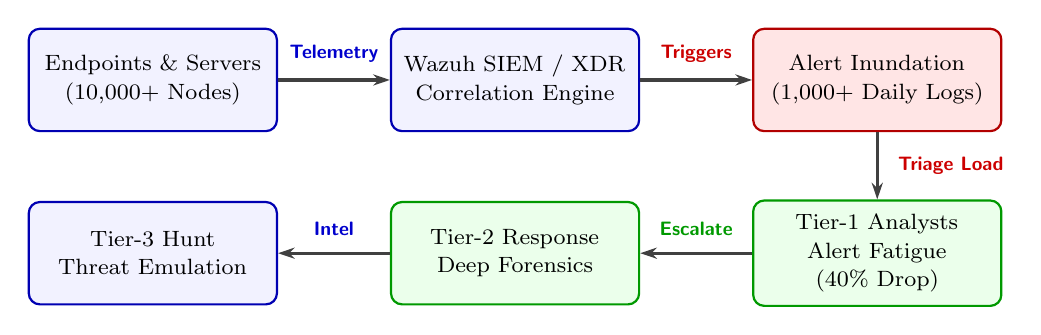
\begin{tikzpicture}[
  box/.style={rectangle, draw=blue!70!black, fill=blue!5, rounded corners=4pt, thick, align=center, font=\footnotesize, text width=2.8cm, minimum height=1.3cm, inner sep=5pt},
  alert/.style={rectangle, draw=red!70!black, fill=red!10, rounded corners=4pt, thick, align=center, font=\footnotesize, text width=2.8cm, minimum height=1.3cm, inner sep=5pt},
  soc/.style={rectangle, draw=green!60!black, fill=green!8, rounded corners=4pt, thick, align=center, font=\footnotesize, text width=2.8cm, minimum height=1.3cm, inner sep=5pt},
  arrow/.style={-{Stealth[length=6pt, width=4pt]}, very thick, draw=black!75},
  lbl/.style={font=\scriptsize\bfseries\sffamily, above=3pt}
]
  % Top Row (Left to Right)
  \node[box] (endpoints) at (0, 0) {Endpoints \& Servers\\(10,000+ Nodes)};
  \node[box] (siem) at (4.6, 0) {Wazuh SIEM / XDR\\Correlation Engine};
  \node[alert] (alerts) at (9.2, 0) {Alert Inundation\\(1,000+ Daily Logs)};

  % Bottom Row (Right to Left)
  \node[soc] (tier1) at (9.2, -2.2) {Tier-1 Analysts\\Alert Fatigue (40\% Drop)};
  \node[soc] (escalate) at (4.6, -2.2) {Tier-2 Response\\Deep Forensics};
  \node[box] (hunt) at (0, -2.2) {Tier-3 Hunt\\Threat Emulation};

  % Connectors
  \draw[arrow] (endpoints.east) -- (siem.west);
  \node[lbl, color=blue!80!black] at ($(endpoints.east)!0.5!(siem.west)$) {Telemetry};

  \draw[arrow] (siem.east) -- (alerts.west);
  \node[lbl, color=red!80!black] at ($(siem.east)!0.5!(alerts.west)$) {Triggers};

  \draw[arrow] (alerts.south) -- (tier1.north);
  \node[font=\scriptsize\bfseries\sffamily\color{red!80!black}, right=4pt] at ($(alerts.south)!0.5!(tier1.north)$) {Triage Load};

  \draw[arrow] (tier1.west) -- (escalate.east);
  \node[lbl, color=green!60!black] at ($(tier1.west)!0.5!(escalate.east)$) {Escalate};

  \draw[arrow] (escalate.west) -- (hunt.east);
  \node[lbl, color=blue!80!black] at ($(escalate.west)!0.5!(hunt.east)$) {Intel};
\end{tikzpicture}%
}
\caption{Traditional multi-tier Security Operations Center triage workflow illustrating the Tier-1 bottleneck.}
\label{fig:soc_workflow_crisis}
\end{figure}

\section{The Alert Inundation Crisis in Security Operations Centers}
\label{sec:alert_crisis}
A Security Operations Center functions as the operational hub of cyber defense, conventionally divided into three hierarchical tiers:
\begin{enumerate}
  \item \textbf{Tier-1 Alert Triage Analysts:} Frontline operators responsible for monitoring real-time queues, validating alarms, distinguishing malicious signals from benign noise, and escalating high-fidelity incidents.
  \item \textbf{Tier-2 Incident Responders:} Forensics specialists who analyze escalated alerts, establish blast radiuses, and execute containment playbooks.
  \item \textbf{Tier-3 Threat Hunters:} Strategic engineers who identify dormant threats, build custom detection rules, and conduct root-cause assessments.
\end{enumerate}

Despite this structured division of labor, modern SOCs face a crippling bottleneck at the Tier-1 level. SIEM correlation rules prioritize detection sensitivity over specificity to prevent missed compromises. Consequently, correlation engines generate massive volumes of false positives, benign routine sysadmin alarms, and non-actionable notifications. Industry benchmarks indicate that analysts process upwards of 1,000 alerts per shift. Human cognitive limits induce severe ``alert fatigue,'' requiring 15--25 minutes to manually investigate a single event. Consequently, up to 40\% of alerts are dismissed without thorough investigation, drastically expanding adversary dwell time.

\section{Risks and Deficiencies of Commercial Cloud AI Copilots}
\label{sec:cloud_ai_risks}
The emergence of generative Large Language Models (LLMs) has prompted growing interest in AI-assisted triage. However, commercial cloud-hosted models introduce critical vulnerabilities into enterprise SOC operations:
\begin{enumerate}
  \item \textbf{Data Privacy and Sovereignty Breaches:} SIEM alerts contain confidential internal IP schemas, server hostnames, employee usernames, connection strings, and session tokens. Egressing this telemetry to external cloud APIs violates GDPR, SOC2 Type II, HIPAA, and sovereign data regulations.
  \item \textbf{Generative Hallucinations:} Unconstrained generative models hallucinate plausible but non-existent CVEs or misattribute benign scripts to catastrophic attack techniques, misguiding junior analysts.
  \item \textbf{Absence of Verifiable Grounding:} Commercial chat APIs provide conversational summaries without mathematical proof that claims originate from authoritative threat documentation (such as MITRE ATT\&CK or NIST NVD).
\end{enumerate}

\section{Problem Statement}
\label{sec:problem_statement}
To eliminate alert fatigue without cloud data exposure, enterprise defense requires a localized, sovereign triage assistant. However, naively coupling an open-weights LLM to a local vector store via standard dense Retrieval-Augmented Generation (RAG) fails in cybersecurity. Repetitive, generic system tokens (\texttt{failed}, \texttt{sshd}, \texttt{connection}, \texttt{port 22}) induce severe \textbf{semantic drift} in vector spaces, obscuring genuine adversary behaviors and suppressing ground-truth knowledge chunks.

The core research question investigated in this work is:
\begin{quote}
\itshape
How can an on-premise, zero-cloud Security Operations Center assistant achieve high-fidelity threat classification, authoritative vulnerability grounding, and verifiable citation governance over noisy enterprise security telemetry without succumbing to semantic retrieval drift or compromising institutional data privacy?
\end{quote}

\section{Project Objectives}
\label{sec:objectives}
To address this challenge, four primary research and engineering objectives are defined:
\begin{enumerate}
  \item \textbf{Sovereign On-Premise System Engineering:} Implement an end-to-end containerized platform featuring FastAPI, PostgreSQL, Qdrant, and Ollama serving Qwen3:8B, guaranteeing zero external cloud egress.
  \item \textbf{Entity-Anchored Dual Retrieval:} Engineer a hybrid retrieval mechanism extracting alert observables (IPs, users, rule tags, technique IDs) to anchor Qdrant vector search, eliminating semantic drift.
  \item \textbf{Verifiable Citation Governance:} Construct an automated verification engine that cross-examines LLM-generated citations against retrieved chunk IDs, trapping and penalizing hallucinations before persistence.
  \item \textbf{Empirical Tri-Mode Evaluation:} Execute an audited 120-run benchmark across 40 enterprise scenarios under three operational paradigms alongside an isolated 40-scenario retrieval ablation over 1,762 indexed security chunks.
\end{enumerate}

\begin{table}[!htbp]
\centering
\caption{System objectives and their corresponding architectural implementations.}
\label{tab:objectives_alignment}
\small
\begin{tabularx}{\textwidth}{@{}l p{4.2cm} X@{}}
\toprule
\textbf{No.} & \textbf{Core Objective} & \textbf{Architectural Implementation} \\
\midrule
1 & Sovereign Privacy & Fully local execution using FastAPI, PostgreSQL, Qdrant, and Ollama (\texttt{qwen3:8b}); zero external cloud calls. \\
2 & Semantic Drift Resolution & Entity-Anchored Dual Retrieval combining exact payload filtering with dense vector search in Qdrant. \\
3 & Advisory Triage Support & Automated generation of standardized incident summaries, severity ratings, MITRE mappings, and non-destructive containment playbooks. \\
4 & Auditability \& Governance & Automated citation validation verifying reference-ID existence in threat documentation (97.3\% valid reference rate). \\
5 & Rigorous Empirical Validation & Controlled 120-run benchmark across 40 Dataset v2 scenarios with complete statistical provenance and failure analysis. \\
\bottomrule
\end{tabularx}
\end{table}

\section{Scope and Delimitations}
\label{sec:scope}
The operational boundaries of this research are:
\begin{itemize}
  \item \textbf{Advisory Decision Support:} The assistant provides human-in-the-loop triage support; it never executes destructive network blocking without analyst authorization.
  \item \textbf{Local Computational Envelope:} The architecture executes efficiently on commodity host hardware (CPU and single-GPU), balancing inference latency against model scale.
  \item \textbf{Standardized Security Taxonomies:} Knowledge retrieval is anchored in the MITRE ATT\&CK Enterprise Matrix v14.1 (1,618 chunks) and NIST NVD (144 CVE chunks).
  \item \textbf{Delimitations:} Autonomous threat hunting over unparsed packet streams is excluded; input telemetry conforms to structured Wazuh SIEM schemas.
\end{itemize}

\section{Major Technical Contributions}
\label{sec:contributions}
The specific academic and engineering contributions of this project are:
\begin{enumerate}
  \item \textbf{Entity-Anchored Retrieval Leap:} Proving empirically that observable anchoring delivers a \textbf{+67.5 percentage-point increase in Recall@1} (from 22.5\% under dense RAG to 90.0\%) across 1,762 security chunks.
  \item \textbf{Sovereign Air-Gapped Architecture:} Demonstrating a production-grade on-premise SOC copilot with sub-second retrieval latency and real-time Server-Sent Events (SSE) streaming.
  \item \textbf{Verifiable Citation Governance Engine:} Establishing an automated validation layer enforcing a 97.3\% citation veracity rate and preventing hallucinated vulnerability references.
  \item \textbf{Forensic Failure Attribution:} Documenting why high retrieval accuracy does not linearly inflate classification F1, analyzing context distractor effects (Case 20) and JSON syntax fallbacks (Case 24).
\end{enumerate}

\section{Organization of the Report}
\label{sec:org}
The remainder of this report is organized as follows:
\begin{itemize}
  \item \textbf{Chapter \ref{ch:literature}} surveys prior work in SIEM platforms, LLM security copilots, and the SERC base paper.
  \item \textbf{Chapter \ref{ch:theory}} presents mathematical formulations of self-attention, HNSW indexing, and evaluation metrics.
  \item \textbf{Chapter \ref{ch:architecture}} details the four-tier sovereign architecture, database schemas, and REST/SSE APIs.
  \item \textbf{Chapter \ref{ch:implementation}} specifies the end-to-end methodology, entity extraction, and retrieval algorithms.
  \item \textbf{Chapter \ref{ch:experiments}} describes Dataset v2 composition, scenario distributions, and benchmark integrity fixes.
  \item \textbf{Chapter \ref{chap:results_evaluation}} analyzes empirical findings, retrieval ablations, latency profiles, and failure cases.
  \item \textbf{Chapter \ref{chap:testing_security}} details the 264-test automated verification suite and STRIDE threat modeling.
  \item \textbf{Chapter \ref{chap:limitations_future_work}} discusses operational trade-offs and future engineering directions.
  \item \textbf{Chapter \ref{chap:conclusion}} concludes the report with a summary of scientific achievements.
\end{itemize}
%==============================================================================
% Chapter 2: Literature Review
%==============================================================================
\chapter{Literature Review}
\label{ch:literature}

\section{Traditional Security Operations Center Workflows}
\label{sec:lit_traditional_soc}
The architectural foundation of enterprise Security Operations Centers stems from defense-in-depth doctrines. Traditional SOC operations rely on event aggregation, where distributed agents forward system logs to a centralized Security Information and Event Management (SIEM) appliance. As formulated by NIST SP 800-61 Revision 2 \cite{nist_sp800_61}, the incident response lifecycle comprises four discrete phases: preparation, detection and analysis, containment and recovery, and post-incident activity.

In operational practice, detection and analysis represent the primary operational bottleneck. Early SIEM systems utilized static threshold rules. While simple to deploy, static correlation suffers from critical vulnerabilities:
\begin{itemize}
  \item \textbf{Inflexibility against Novel Attacks:} Static rules fail against zero-day exploits or polymorphic malware deviating from hardcoded thresholds.
  \item \textbf{High False-Alarm Rates:} Routine system maintenance and benign administrative scripts regularly trigger alarms, inundating analyst queues \cite{sarker2023soc}.
  \item \textbf{Contextual Fragmentation:} Rule triggers generate isolated alerts without linking them to broader threat intelligence, forcing manual multi-database queries.
\end{itemize}

\section{The Wazuh Open-Source SIEM and XDR Platform}
\label{sec:lit_wazuh}
To eliminate the high licensing costs of proprietary SIEMs, enterprise security teams have widely adopted open-source XDR platforms, predominantly \textbf{Wazuh} \cite{wazuh_siem_xdr}. Wazuh provides host and network monitoring via lightweight agents deployed across Linux, Windows, macOS, and container environments. Its architecture comprises three primary tiers:
\begin{enumerate}
  \item \textbf{Wazuh Agents:} Endpoint daemons performing log collection, file integrity monitoring (FIM), rootkit detection, and system configuration checks.
  \item \textbf{Wazuh Server (Manager):} Centralized analysis cluster executing an XML-based decoding and ruleset engine, assigning severity ratings ($0 \le s \le 16$) and tagging events with MITRE ATT\&CK technique IDs (\texttt{rule.mitre.id}).
  \item \textbf{Wazuh Indexer and Dashboard:} An OpenSearch-based distributed storage and analytics engine storing alerts as JSON documents with interactive visualization.
\end{enumerate}
Despite these capabilities, Wazuh remains a passive correlation system. It cannot automatically generate natural-language incident summaries or infer multi-stage adversary progression across disparate event streams.

\section{Large Language Models in Cybersecurity Operations}
\label{sec:lit_llm_cyber}
The development of transformer-based Large Language Models (LLMs) \cite{vaswani2017attention} has transformed natural language understanding and domain reasoning. In cybersecurity, researchers have explored foundational models for log parsing, threat intelligence synthesis, and vulnerability triage \cite{ferrag2024generativeai}. Foundational models exhibit strong parametric knowledge of software internals, protocol mechanics, and common attack vectors \cite{albert2023copilot}.

However, deploying unaugmented foundational models in enterprise SOCs reveals severe operational flaws:
\begin{itemize}
  \item \textbf{Parametric Knowledge Cutoffs:} Models possess knowledge restricted to their training corpora; newly disclosed CVEs and novel zero-day campaigns are absent.
  \item \textbf{Generative Hallucinations:} When prompted regarding unfamiliar threats, unaugmented models invent realistic-looking CVE numbers and non-existent technique IDs \cite{ferrag2024generativeai}.
  \item \textbf{Absence of Verifiable Grounding:} Raw LLMs cannot provide cryptographic or source-identifier proof for their recommendations, preventing analyst validation.
\end{itemize}

\section{Retrieval-Augmented Generation (RAG) in Threat Analysis}
\label{sec:lit_rag}
To resolve parametric cutoffs and hallucinations, Lewis et al.\ \cite{lewis2020rag} introduced \textbf{Retrieval-Augmented Generation (RAG)}. Under this paradigm, authoritative documents are pre-indexed into a dense vector space. For each incoming query, the system retrieves the top-$k$ most semantically relevant chunks and injects them into the prompt context before inference.

In cybersecurity, RAG enables an LLM to reference up-to-date threat catalogs (such as the MITRE ATT\&CK framework and NIST NVD) without model retraining \cite{tarek2024cve}. By grounding model reasoning in retrieved external evidence, RAG curbs hallucinations, surfaces inspectable source citations, and allows organizations to inject internal network playbooks dynamically.

\begin{figure}[!htbp]
\centering
\resizebox{0.96\textwidth}{!}{%
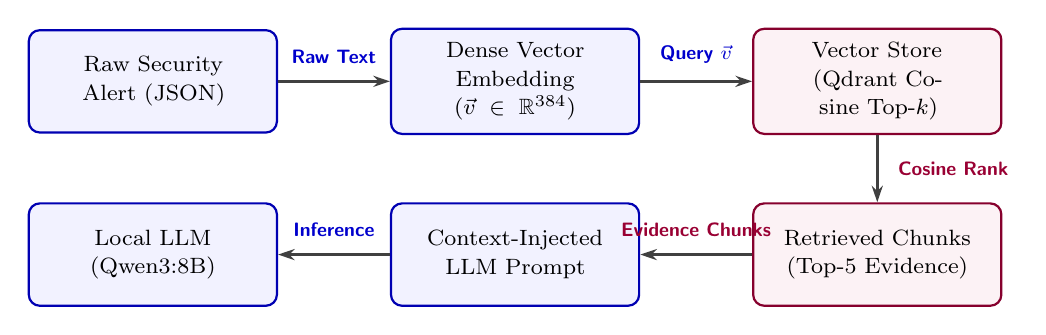
\begin{tikzpicture}[
  box/.style={rectangle, draw=blue!70!black, fill=blue!5, rounded corners=4pt, thick, align=center, font=\footnotesize, text width=2.8cm, minimum height=1.3cm, inner sep=5pt},
  rag/.style={rectangle, draw=purple!70!black, fill=purple!5, rounded corners=4pt, thick, align=center, font=\footnotesize, text width=2.8cm, minimum height=1.3cm, inner sep=5pt},
  arrow/.style={-{Stealth[length=6pt, width=4pt]}, very thick, draw=black!75},
  lbl/.style={font=\scriptsize\bfseries\sffamily, above=3pt}
]
  % Top Row (Left to Right)
  \node[box] (alert) at (0, 0) {Raw Security\\Alert (JSON)};
  \node[box] (embed) at (4.6, 0) {Dense Vector\\Embedding ($\vec{v} \in \mathbb{R}^{384}$)};
  \node[rag] (qdrant) at (9.2, 0) {Vector Store\\(Qdrant Cosine Top-$k$)};

  % Bottom Row (Right to Left)
  \node[rag] (chunks) at (9.2, -2.2) {Retrieved Chunks\\(Top-5 Evidence)};
  \node[box] (prompt) at (4.6, -2.2) {Context-Injected\\LLM Prompt};
  \node[box] (llm) at (0, -2.2) {Local LLM\\(Qwen3:8B)};

  % Connectors
  \draw[arrow] (alert.east) -- (embed.west);
  \node[lbl, color=blue!80!black] at ($(alert.east)!0.5!(embed.west)$) {Raw Text};

  \draw[arrow] (embed.east) -- (qdrant.west);
  \node[lbl, color=blue!80!black] at ($(embed.east)!0.5!(qdrant.west)$) {Query $\vec{v}$};

  \draw[arrow] (qdrant.south) -- (chunks.north);
  \node[font=\scriptsize\bfseries\sffamily\color{purple!80!black}, right=4pt] at ($(qdrant.south)!0.5!(chunks.north)$) {Cosine Rank};

  \draw[arrow] (chunks.west) -- (prompt.east);
  \node[lbl, color=purple!80!black] at ($(chunks.west)!0.5!(prompt.east)$) {Evidence Chunks};

  \draw[arrow] (prompt.west) -- (llm.east);
  \node[lbl, color=blue!80!black] at ($(prompt.west)!0.5!(llm.east)$) {Inference};
\end{tikzpicture}%
}
\caption{Conventional Unanchored Dense RAG pipeline for security telemetry, vulnerable to semantic drift.}
\label{fig:standard_rag_drift}
\end{figure}

\section{Analysis of the Base Paper: Wazuh SERC Copilot (Sensors, 2025)}
\label{sec:lit_base_paper}
A primary conceptual foundation of this project is the study by Al-Mohannadi et al.\ in \emph{Sensors} (MDPI, 2025), entitled: \emph{``Enhancing Security Operations Center: Wazuh Security Event Response with Retrieval-Augmented-Generation-Driven Copilot''} \cite{sensors2025wazuhcopilot}. The authors proposed the \textbf{Security Event Response Copilot (SERC)} to bridge the operational gap between raw Wazuh telemetry and incident mitigation. SERC structures knowledge across three vector databases:
\begin{enumerate}
  \item \textbf{General Incident Response Knowledge Base:} Practical remediation guides and emergency containment playbooks.
  \item \textbf{NIST CSF 2.0 Knowledge Base:} Standardized regulatory lifecycle mappings.
  \item \textbf{MITRE ATT\&CK Knowledge Base:} Taxonomic descriptions of adversary TTPs.
\end{enumerate}
When Wazuh fires an alert, SERC extracts the rule description, queries these multi-framework stores, and prompts an LLM to generate mitigation playbooks.

\section{Research Gaps and Limitations of Prior Work}
\label{sec:lit_gaps}
While SERC \cite{sensors2025wazuhcopilot} demonstrates the potential of RAG-assisted triage, our forensic analysis reveals several fundamental scientific and architectural gaps in existing literature:
\begin{enumerate}
  \item \textbf{Semantic Drift in Security Telemetry:} Standard RAG applies unconstrained dense similarity to raw log strings. However, security logs are saturated with non-discriminative syntax tokens (\texttt{authentication}, \texttt{failed}, \texttt{sshd}, \texttt{root}). Dense sentence encoders project these generic tokens into dominant clusters, causing the embedding to reflect protocol mechanics rather than malicious behavior. Consequently, ground-truth threat chunks frequently drop outside the top-$k$ retrieval window.
  \item \textbf{Cloud Dependency and Sovereignty Risks:} Existing architectures frequently route telemetry to commercial cloud APIs, breaching enterprise data privacy regulations.
  \item \textbf{Absence of Citation Governance:} Prior systems rely on unsupervised generative citations. In practice, LLMs regularly hallucinate non-existent citation IDs without automated validation.
  \item \textbf{Conflation of Retrieval and Generation Metrics:} Prior studies report high retrieval scores and assume end-to-end classification improved proportionally, lacking isolated ablations on identical, controlled benchmarks.
\end{enumerate}

\begin{table}[!htbp]
\centering
\caption{Comparative analysis: Traditional SOC, Cloud Copilots, Base Paper (SERC), and Sovereign Assistant.}
\label{tab:lit_comparison}
\small
\begin{tabularx}{\textwidth}{@{}l p{3.2cm} p{3.2cm} X@{}}
\toprule
\textbf{Dimension} & \textbf{Cloud Copilots} & \textbf{Wazuh SERC \cite{sensors2025wazuhcopilot}} & \textbf{Proposed Sovereign Assistant} \\
\midrule
\textbf{Execution} & Third-Party Cloud API & Cloud / Hybrid LLM & \textbf{100\% Sovereign On-Premise (Local)} \\
\textbf{Data Egress} & High Risk (External) & Moderate Risk & \textbf{Zero Egress (Air-gapped capable)} \\
\textbf{Retrieval} & Generic Dense RAG & Multi-Collection Dense & \textbf{Entity-Anchored Dual Retrieval} \\
\textbf{Recall@1} & Unmeasured in logs & $\approx 20\text{--}30\%$ (Drift) & \textbf{90.0\% (Verified +67.5 pp leap)} \\
\textbf{Governance} & None (Trust LLM) & Static Prompting & \textbf{Automated Citation Engine (97.3\%)} \\
\textbf{CVE Grounding} & Unreliable hallucinations & Qualitative Playbooks & \textbf{Empirical Log4Shell (1.00 F1)} \\
\textbf{Testing} & Black-box evaluation & Qualitative cases & \textbf{264 Automated Tests + Audited Runs} \\
\bottomrule
\end{tabularx}
\end{table}

\section{Motivation for Entity-Anchored Dual Retrieval}
\label{sec:lit_motivation_anchoring}
To eliminate semantic drift, this research introduces \textbf{Entity-Anchored Dual Evidence Retrieval}. Rather than submitting unparsed alert strings to dense embedding models, our architecture deterministically extracts structured operational observables—specifically IP addresses, usernames, rule severity, process paths, and Wazuh technique tags (\texttt{rule.mitre.id}).

By decomposing telemetry into structured entities, the retriever executes a dual-pass query in Qdrant:
\begin{enumerate}
  \item An \textbf{exact payload-filtered search} targeting specific MITRE ATT\&CK IDs and CVE patterns.
  \item A \textbf{dense semantic vector search} targeting descriptive attack terms and normalized event categories.
\end{enumerate}
These candidate sets are merged, deduplicated, and ranked by genuine cosine similarity. As established in Chapter \ref{chap:results_evaluation}, this formulation increases Top-1 Retrieval Recall from 22.5\% under standard dense RAG to \textbf{90.0\%}, establishing an empirically validated foundation for sovereign SOC triage.
%==============================================================================
% Chapter 3: Theoretical Background and Mathematical Foundations
%==============================================================================
\chapter{Theoretical Background and Mathematical Foundations}
\label{ch:theory}

\section{Security Telemetry and SIEM Event Normalization}
\label{sec:theory_telemetry}
Security Information and Event Management systems collect telemetry across heterogeneous operating systems, network appliances, and authentication daemons. Raw system logs are semi-structured text strings that vary across platforms (e.g., Linux Syslog vs.\ Windows Event ID 4625). Machine reasoning requires standardizing raw text into a canonical schema. The normalized security event $\mathcal{E}$ is formally defined as:
\begin{equation}
\label{eq:alert_tuple}
\mathcal{E} = \left( t_{\text{event}}, \text{src}_{\text{ip}}, \text{dst}_{\text{ip}}, \text{src}_{\text{port}}, \text{dst}_{\text{port}}, u, h_{\text{agent}}, s_{\text{severity}}, \mathcal{M}_{\text{tags}}, \mathcal{D}_{\text{desc}} \right)
\end{equation}
Where $t_{\text{event}}$ is the UTC timestamp; $\text{src}_{\text{ip}}, \text{dst}_{\text{ip}} \in \mathcal{IP}$; $\text{src}_{\text{port}}, \text{dst}_{\text{port}} \in [1, 65535]$; $u$ is the principal username; $h_{\text{agent}}$ denotes the hostname and OS; $s_{\text{severity}} \in [0, 16]$ is the standardized Wazuh severity level; $\mathcal{M}_{\text{tags}} \subset \{\text{T1000}, \dots, \text{T1999}\}$ represents pre-tagged MITRE ATT\&CK technique IDs; and $\mathcal{D}_{\text{desc}}$ is the rule description.

\section{Large Language Models and Transformer Decoders}
\label{sec:theory_llm}
The language models utilized in this research are autoregressive causal decoders rooted in the multi-head self-attention transformer architecture \cite{vaswani2017attention}. For input tokens $\mathbf{x} = (x_1, \dots, x_n)$, contextual projections yield Query ($\mathbf{Q}$), Key ($\mathbf{K}$), and Value ($\mathbf{V}$) matrices via parameter weights $W_Q, W_K, W_V \in \mathbb{R}^{d_{\text{model}} \times d_k}$.

Scaled dot-product attention is defined as:
\begin{equation}
\label{eq:scaled_attention}
\text{Attention}(\mathbf{Q}, \mathbf{K}, \mathbf{V}) = \text{softmax}\left( \frac{\mathbf{Q} \mathbf{K}^T}{\sqrt{d_k}} + \mathbf{M} \right) \mathbf{V}
\end{equation}
Where $d_k$ is the scaling factor, and $\mathbf{M} \in \mathbb{R}^{n \times n}$ is an upper-triangular causal attention mask ($M_{ij} = -\infty$ for $j > i$ and $0$ otherwise). Multi-Head Attention (MHA) concatenates $h$ parallel projections:
\begin{equation}
\label{eq:mha}
\text{MHA}(\mathbf{Q}, \mathbf{K}, \mathbf{V}) = \text{Concat}(\text{head}_1, \dots, \text{head}_h) W_O
\end{equation}
Our local inference engine serves \textbf{Qwen3:8B} via Ollama \cite{qwen2024technical}, employing RoPE embeddings, SwiGLU activations, and Grouped-Query Attention (GQA). To guarantee deterministic evaluation, decoding temperature is constrained to $T = 0.0$ (greedy decoding):
\begin{equation}
\label{eq:greedy_decoding}
x_{n+1} = \arg\max_{w \in \mathcal{V}} P(w \mid x_1, \dots, x_n)
\end{equation}

\section{Dense Vector Embeddings and Semantic Metric Spaces}
\label{sec:theory_embeddings}
To perform semantic search across threat intelligence, text is projected into a continuous low-dimensional vector space via the \textbf{all-MiniLM-L6-v2} sentence transformer \cite{reimers2019sentencebert}. Given text $S$, token embeddings $\mathbf{h}_1, \dots, \mathbf{h}_L \in \mathbb{R}^{384}$ are mean-pooled into sentence vector $\mathbf{e}$:
\begin{equation}
\label{eq:mean_pooling}
\mathbf{e} = \frac{1}{L} \sum_{i=1}^L \mathbf{h}_i, \quad \mathbf{v} = \frac{\mathbf{e}}{\|\mathbf{e}\|_2} = \frac{\mathbf{e}}{\sqrt{\sum_{j=1}^{384} e_j^2}}
\end{equation}
Semantic similarity between query vector $\mathbf{v}_q$ and document vector $\mathbf{v}_d$ is computed via Cosine Similarity:
\begin{equation}
\label{eq:cosine_sim}
\text{Sim}(\mathbf{v}_q, \mathbf{v}_d) = \cos(\theta) = \frac{\mathbf{v}_q \cdot \mathbf{v}_d}{\|\mathbf{v}_q\|_2 \|\mathbf{v}_d\|_2} = \sum_{j=1}^{384} v_{q,j} \cdot v_{d,j} \in [-1, 1]
\end{equation}
In Qdrant, Cosine Distance is defined as $D_{\text{cosine}}(\mathbf{v}_q, \mathbf{v}_d) = 1 - \text{Sim}(\mathbf{v}_q, \mathbf{v}_d) \in [0, 2]$.

\section{Vector Indexing and Hierarchical Navigable Small World Graphs}
\label{sec:theory_hnsw}
Exact nearest neighbor search across thousands of high-dimensional vectors has linear complexity $\mathcal{O}(N \cdot d)$. To achieve sub-second search, \textbf{Qdrant} utilizes \textbf{Hierarchical Navigable Small World (HNSW)} graph indexing \cite{malkov2018hnsw}. HNSW organizes vectors into hierarchical layers $\mathcal{L}_0, \dots, \mathcal{L}_{k_{\text{max}}}$, where upper layers support rapid long-range greedy routing toward the query vector $\mathbf{v}_q$, descending sequentially until layer $\mathcal{L}_0$. Bitset filtering is evaluated directly during graph traversal, pruning non-matching nodes without corrupting connectivity and achieving $\mathcal{O}(\log N)$ logarithmic search complexity.

\section{Lexical Retrieval and Deterministic Token Hashing}
\label{sec:theory_hashing}
As an offline, non-neural baseline, we implement a deterministic \textbf{Hashing Embedding Provider} mapping text into fixed-dimension vectors $\mathbf{u} \in \mathbb{R}^{256}$ via character bigram feature hashing:
\begin{equation}
\label{eq:ngrams}
\mathcal{G}(S) = \{c_i c_{i+1} \mid c_i \in \text{tokens}(S)\}
\end{equation}
For each bigram $g$, an MD5 digest $H(g) = (b_0, \dots, b_{15})$ assigns feature indices:
\begin{equation}
\label{eq:hash_indices}
i_A = \text{int}(b_0 \dots b_3) \pmod d, \quad i_B = \text{int}(b_4 \dots b_7) \pmod d
\end{equation}
\begin{equation}
\label{eq:hash_accum}
u_{i_A} \leftarrow u_{i_A} + s, \qquad u_{i_B} \leftarrow u_{i_B} - s
\end{equation}
Where pseudo-random sign $s = (-1)^{b_8 \pmod 2}$ disperses feature variance across the vector. Normalized vector $\mathbf{u}$ serves as an ultra-fast lexical baseline ($38.9\text{ ms}$) matching exact technique strings.

\section{Mathematical Formulation of Performance Metrics}
\label{sec:theory_metrics}
Rigorous empirical evaluation requires formal definitions of all reported metrics.

\subsection{Classification Metrics (MITRE ATT\&CK Technique Triage)}
Let $\mathcal{C}$ be the MITRE ATT\&CK techniques. For scenario $i$, let $\mathcal{G}_i \subset \mathcal{C}$ be ground-truth techniques, and $\mathcal{P}_i \subset \mathcal{C}$ be predicted techniques across $N$ scenarios:
\begin{equation}
TP = \sum_{i=1}^N |\mathcal{P}_i \cap \mathcal{G}_i|, \quad FP = \sum_{i=1}^N |\mathcal{P}_i \setminus \mathcal{G}_i|, \quad FN = \sum_{i=1}^N |\mathcal{G}_i \setminus \mathcal{P}_i|
\end{equation}
Scenario Precision ($P_i$), Recall ($R_i$), and F1 ($F_{1,i}$) are defined:
\begin{equation}
\label{eq:prec_rec_f1}
P_i = \frac{|\mathcal{P}_i \cap \mathcal{G}_i|}{|\mathcal{P}_i| + \epsilon}, \quad R_i = \frac{|\mathcal{P}_i \cap \mathcal{G}_i|}{|\mathcal{G}_i| + \epsilon}, \quad F_{1,i} = \frac{2 P_i R_i}{P_i + R_i + \epsilon}
\end{equation}
Where $\epsilon = 10^{-9}$ handles negative control scenarios ($\mathcal{P}_i = \emptyset, \mathcal{G}_i = \emptyset$). Macro metrics average individual scenario scores ($\text{Macro } F_1 = \frac{1}{N} \sum F_{1,i}$), while Micro metrics aggregate global counts ($\text{Micro } F_1 = \frac{2 TP}{2 TP + FP + FN}$).

\subsection{Information Retrieval Ranking Metrics}
In retrieval ablation, candidate rankings $\mathcal{R} = (r_1, \dots, r_K)$ from knowledge base $\mathcal{K}$ ($|\mathcal{K}| = 1,762$) are evaluated against ground-truth chunks $\mathcal{G}$:
\begin{equation}
\label{eq:recall_at_k}
\text{Recall}@k = \frac{1}{|Q|} \sum_{q=1}^{|Q|} \mathbb{I}\left( \exists r_j \in \mathcal{G}_q \text{ s.t. } j \le k \right)
\end{equation}
\begin{equation}
\label{eq:mrr}
\text{RR}_q = \frac{1}{\min \{j \mid r_j \in \mathcal{G}_q\}}, \quad \text{MRR} = \frac{1}{|Q|} \sum_{q=1}^{|Q|} \text{RR}_q
\end{equation}

\subsection{Latency Profiling and Statistical Separation}
Timing is measured across two distinct regimes: sub-second \textbf{Retrieval Latency} ($t_{\text{search}}$ in milliseconds) and multi-second \textbf{End-to-End Triage Latency} ($t_{\text{triage}}$ in seconds), evaluated via sample mean ($\mu$) and standard deviation ($\sigma$):
\begin{equation}
\label{eq:latency_stats}
\mu = \frac{1}{N} \sum_{i=1}^N t_i, \quad \sigma = \sqrt{\frac{1}{N-1} \sum_{i=1}^N (t_i - \mu)^2}
\end{equation}
%==============================================================================
% Chapter 4: System Requirements and Architecture
%==============================================================================
\chapter{System Requirements and Architecture}
\label{ch:architecture}

\section{Requirements Analysis}
\label{sec:requirements_analysis}
Designing an on-premise AI-assisted SOC platform requires balancing continuous streaming telemetry with the computational demands of local deep neural network inference. The operational specifications are partitioned into functional and non-functional requirements.

\subsection{Functional Requirements}
\begin{enumerate}[itemsep=1pt,topsep=2pt]
  \item \textbf{Telemetry Ingestion and Normalization:} Ingest raw events from Wazuh SIEM, Syslog daemons, or replay datasets, normalizing them into canonical \texttt{NormalizedSecurityAlert} schemas.
  \item \textbf{Deterministic Context Extraction:} Deterministically extract observables (IPs, ports, hostnames, usernames, process paths, and MITRE technique tags) without external lookups.
  \item \textbf{Categorized Query Construction:} Synthesize structured queries spanning MITRE techniques, CVE identifiers, and general security terms.
  \item \textbf{Hybrid Vector Retrieval:} Execute semantic similarity search in Qdrant with exact payload filtering.
  \item \textbf{Tri-Mode Analysis Orchestration:} Support LLM-Only, Standard RAG, and Evidence-Aware RAG under identical inputs.
  \item \textbf{Automated Citation Governance:} Inspect generated incident rationales, verify that every cited evidence identifier exists within retrieved sets, and penalize fabricated references.
  \item \textbf{Persistent Storage and Source Isolation:} Store analyses and evidence in PostgreSQL with strict data-source provenance (\texttt{demo}, \texttt{wazuh\_live}, \texttt{replay\_v2}).
  \item \textbf{Real-Time Trace Streaming:} Emit stage-by-stage execution timings via Server-Sent Events (SSE).
  \item \textbf{Analyst Console:} Provide interactive queue triage, D3.js entity graphs, and technical trace waterfalls.
\end{enumerate}

\subsection{Non-Functional Requirements}
\begin{enumerate}[itemsep=1pt,topsep=2pt]
  \item \textbf{Sovereign Privacy:} Guarantee zero cloud data egress; all weights, embeddings, and stores run locally.
  \item \textbf{Sub-Second Retrieval:} Return ranked evidence chunks in under 300 ms to avoid retrieval bottlenecks.
  \item \textbf{Algorithmic Determinism:} Constrain inference to temperature 0.0 for reproducible evaluation.
  \item \textbf{Data Integrity:} Namespace evaluation alerts to prevent benchmark collision.
  \item \textbf{Containerized Portability:} Containerize all microservices via Docker and Docker Compose.
\end{enumerate}

\begin{table}[!htbp]
\centering
\caption{System requirements and operational constraints.}
\label{tab:system_requirements}
\small
\begin{tabularx}{\textwidth}{@{}l p{4.0cm} X@{}}
\toprule
\textbf{Category} & \textbf{Requirement Name} & \textbf{Operational Implementation Specification} \\
\midrule
\textbf{FR-01} & Telemetry Normalization & Parse Wazuh JSON into \texttt{NormalizedSecurityAlert} schema. \\
\textbf{FR-02} & Entity Extraction & Deterministic regex extraction of IPs, ports, users, MITRE IDs. \\
\textbf{FR-03} & Hybrid Vector Search & Qdrant HNSW cosine similarity combined with payload filters. \\
\textbf{FR-04} & Tri-Mode Orchestration & Switchable execution: LLM-Only, Standard RAG, Evidence-Aware. \\
\textbf{FR-05} & Citation Governance & Automated validation verifying citation IDs exist in retrieved set. \\
\textbf{FR-06} & Real-time Trace Streaming & SSE stream emitting JSON trace events for all pipeline stages. \\
\midrule
\textbf{NFR-01} & Zero Cloud Egress & Fully local execution: Ollama (\texttt{qwen3:8b}), local Qdrant, local Postgres. \\
\textbf{NFR-02} & Search Latency & Sub-second vector search: Mean retrieval latency $< 250\text{ ms}$. \\
\textbf{NFR-03} & Schema Versioning & Alembic migration (\texttt{c01\_datasource}) isolating alert sources. \\
\textbf{NFR-04} & Software Reliability & Comprehensive test suite: 264 automated software tests passing. \\
\bottomrule
\end{tabularx}
\end{table}

\section{Hardware and Host Deployment Environment}
\label{sec:hardware_environment}
The platform operates efficiently within standard enterprise on-premise computing envelopes:
\begin{itemize}[itemsep=1pt,topsep=2pt]
  \item \textbf{Processor (CPU):} Multi-core x86\_64 processor (Intel Core i7/i9 or AMD Ryzen 7/9, 8+ physical cores).
  \item \textbf{Memory (RAM):} 16 GB minimum, 32 GB recommended, allocated across PostgreSQL (1 GB), Qdrant (2 GB), FastAPI Backend (2 GB), and Ollama Runtime (8 GB).
  \item \textbf{Accelerator (GPU):} Single NVIDIA GPU with 8+ GB VRAM supporting CUDA compute capability 8.0+ (RTX 3070/4060 or Tesla T4), or quantized CPU inference via Ollama.
  \item \textbf{Storage Subsystem:} High-speed NVMe SSD with 20+ GB storage for indices, weights, and WAL logs.
  \item \textbf{Operating System:} Microsoft Windows 11 Professional (WSL2 Ubuntu 24.04 kernel) or native Linux.
\end{itemize}

\section{Four-Tier Sovereign System Architecture}
\label{sec:tier_architecture}
The system is structured into four functional tiers, illustrated in Figure \ref{fig:architecture_diagram_fig}:
\begin{enumerate}[itemsep=1pt,topsep=2pt]
  \item \textbf{Tier 1: Telemetry Ingestion \& Preprocessing:} Interfaces with log collectors, normalizes event strings into Pydantic models, cleans whitespace, extracts observables, and synthesizes queries.
  \item \textbf{Tier 2: Knowledge Base \& Vector Retrieval:} Houses 1,762 pre-chunked security documents (1,618 MITRE ATT\&CK techniques and 144 NVD CVEs) encoded into 384-dimensional vectors in Qdrant.
  \item \textbf{Tier 3: Reasoning, Governance \& Persistence:} The orchestration engine (\texttt{SOCAnalysisOrchestrator}) compiles prompts, executes Qwen3:8B inference, validates citations, and writes records to PostgreSQL.
  \item \textbf{Tier 4: Analyst Web Console:} React 19 single-page console rendering triage queues, D3 entity graphs, and SSE streaming execution traces.
\end{enumerate}

\begin{figure}[!htbp]
\centering
\resizebox{0.98\textwidth}{!}{%
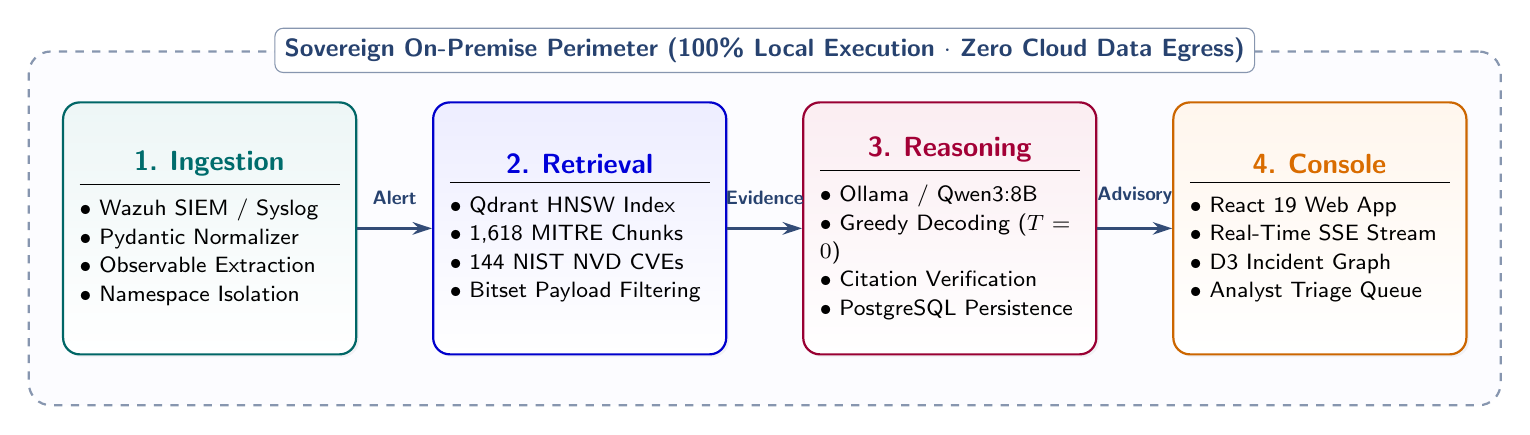
\begin{tikzpicture}[
  tier/.style={
    rectangle, rounded corners=6pt, draw=#1!80!black, top color=#1!7, bottom color=white,
    thick, text width=3.3cm, minimum height=3.2cm, align=left, font=\footnotesize\sffamily,
    inner sep=6pt, drop shadow={opacity=0.08, shadow xshift=1pt, shadow yshift=-1pt}
  },
  arrow/.style={-{Stealth[length=7pt, width=4.5pt]}, very thick, draw=navyblue!85},
  lbl/.style={font=\scriptsize\bfseries\sffamily\color{navyblue!85}, above=3pt}
]

  % Tier 1 Card
  \node[tier=teal] (t1) at (0,0) {
    {\centering\textbf{\color{teal!85!black}\normalsize 1. Ingestion}\par}\vspace{3pt}
    \hrule height 0.4pt\vspace{5pt}
    $\bullet$ Wazuh SIEM / Syslog\\
    $\bullet$ Pydantic Normalizer\\
    $\bullet$ Observable Extraction\\
    $\bullet$ Namespace Isolation
  };

  % Tier 2 Card
  \node[tier=blue] (t2) at (4.7,0) {
    {\centering\textbf{\color{blue!85!black}\normalsize 2. Retrieval}\par}\vspace{3pt}
    \hrule height 0.4pt\vspace{5pt}
    $\bullet$ Qdrant HNSW Index\\
    $\bullet$ 1,618 MITRE Chunks\\
    $\bullet$ 144 NIST NVD CVEs\\
    $\bullet$ Bitset Payload Filtering
  };

  % Tier 3 Card
  \node[tier=purple] (t3) at (9.4,0) {
    {\centering\textbf{\color{purple!85!black}\normalsize 3. Reasoning}\par}\vspace{3pt}
    \hrule height 0.4pt\vspace{5pt}
    $\bullet$ Ollama / Qwen3:8B\\
    $\bullet$ Greedy Decoding ($T=0$)\\
    $\bullet$ Citation Verification\\
    $\bullet$ PostgreSQL Persistence
  };

  % Tier 4 Card
  \node[tier=orange] (t4) at (14.1,0) {
    {\centering\textbf{\color{orange!85!black}\normalsize 4. Console}\par}\vspace{3pt}
    \hrule height 0.4pt\vspace{5pt}
    $\bullet$ React 19 Web App\\
    $\bullet$ Real-Time SSE Stream\\
    $\bullet$ D3 Incident Graph\\
    $\bullet$ Analyst Triage Queue
  };

  % Clean Flow Arrows with Short Centered Labels Cleanly Elevated
  \draw[arrow] (t1.east) -- (t2.west);
  \node[font=\scriptsize\bfseries\sffamily\color{navyblue!90}, above=5pt] at ($(t1.east)!0.5!(t2.west)$) {Alert};

  \draw[arrow] (t2.east) -- (t3.west);
  \node[font=\scriptsize\bfseries\sffamily\color{navyblue!90}, above=5pt] at ($(t2.east)!0.5!(t3.west)$) {Evidence};

  \draw[arrow] (t3.east) -- (t4.west);
  \node[font=\scriptsize\bfseries\sffamily\color{navyblue!90}, above=5pt] at ($(t3.east)!0.5!(t4.west)$) {Advisory};

  % Clean Sovereign Perimeter Frame
  \begin{scope}[on background layer]
    \node[draw=navyblue!50, dashed, thick, rounded corners=8pt, fill=blue!1!white,
          fit=(t1) (t4), inner xsep=12pt, inner ysep=18pt] (frame) {};
  \end{scope}

  % Sovereign Perimeter Header Label (cleanly positioned above frame border)
  \node[font=\small\bfseries\sffamily\color{navyblue!90}, fill=white, draw=navyblue!50, rounded corners=3pt, inner sep=3.5pt]
    at (frame.north) {Sovereign On-Premise Perimeter (100\% Local Execution $\cdot$ Zero Cloud Data Egress)};

\end{tikzpicture}%
}
\caption{Overall Four-Tier Sovereign Architecture of the AI-Powered SOC Assistant, illustrating zero cloud egress across Ingestion, Knowledge, Reasoning, and Presentation layers.}
\label{fig:architecture_diagram_fig}
\end{figure}

\section{Backend Architecture and Asynchronous Pipeline Execution}
\label{sec:backend_arch}
The backend service is engineered in Python 3.11 using \textbf{FastAPI} for native \texttt{asyncio} concurrency and streaming SSE delivery. The codebase is organized modularly:
\begin{itemize}[itemsep=1pt,topsep=2pt]
  \item \texttt{app.main}: Application lifecycle manager, initializing connection pools and CORS middleware.
  \item \texttt{app.api.routes}: 21 REST endpoints grouped into alerts, analyses, datasources, evaluation, health, knowledge, and dashboard.
  \item \texttt{app.security}: Normalization, observable extraction (\texttt{ContextExtractor}), and query synthesis (\texttt{RetrievalQueryBuilder}).
  \item \texttt{app.rag}: Vector retrieval engine (\texttt{Retriever}), embedding adapters, and STIX/NVD chunking pipelines.
  \item \texttt{app.llm}: Local LLM abstraction layer communicating with Ollama HTTP endpoints.
  \item \texttt{app.services}: Core orchestrator (\texttt{SOCAnalysisOrchestrator}) and database CRUD layers.
\end{itemize}

\section{Relational Database Architecture and Schema Isolation}
\label{sec:database_arch}
Incident persistence is managed by \textbf{PostgreSQL 15} via SQLAlchemy 2.0 with the \texttt{asyncpg} driver. The schema comprises three relational tables:
\begin{enumerate}[itemsep=1pt,topsep=2pt]
  \item \textbf{\texttt{alerts} Table:} Ingested events, raw JSON payloads, normalized network tuples, severity, and the \texttt{data\_source} column.
  \item \textbf{\texttt{analyses} Table:} Generated analyses linked via foreign key (\texttt{alert\_id}), storing summaries, severity, reasoning prose, investigation steps, and confidence.
  \item \textbf{\texttt{evidence} Table:} Grounding chunks cited by an analysis linked via foreign key (\texttt{analysis\_id}), storing source metadata, relevance scores, and citations.
\end{enumerate}

\subsection{Database Migration \texttt{c01\_datasource} and Data Isolation}
During Stage 1 auditing, benchmark evaluations were observed colliding with historical demo alerts. Alembic migration \texttt{c01\_datasource} added an indexed \texttt{data\_source} column, strictly isolating records into three namespaces:
\begin{itemize}[itemsep=1pt,topsep=2pt]
  \item \texttt{demo}: Interactive demonstration alerts for user interface testing.
  \item \texttt{wazuh\_live}: Real-time alerts ingested from external Wazuh SIEM clusters.
  \item \texttt{replay\_v2}: Audited benchmark scenarios namespaced as \texttt{v2-eval-001} through \texttt{v2-eval-040}.
\end{itemize}

\begin{figure}[!htbp]
\centering
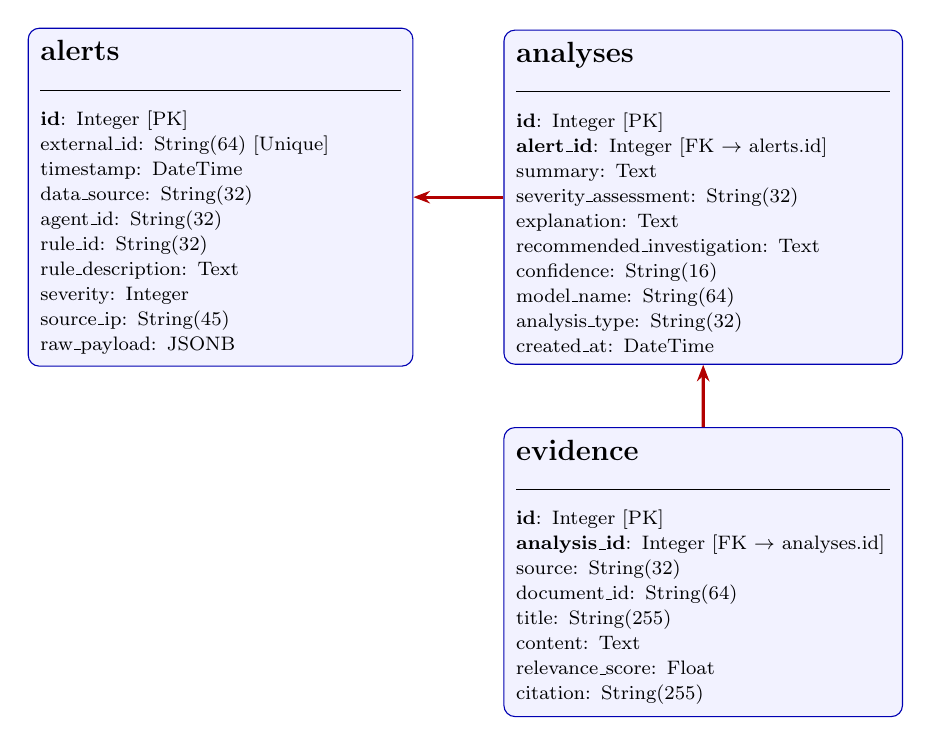
\begin{tikzpicture}[
  scale=0.88, transform shape,
  table/.style={rectangle, draw=blue!70!black, fill=blue!5, rounded corners=4pt, font=\footnotesize, align=left, inner sep=5pt},
  fk/.style={-{Stealth[length=6pt]}, very thick, draw=red!70!black}
]
  \node[table, text width=5.2cm] (alerts) {
    \textbf{\large alerts}\\[2pt]
    \rule{5.2cm}{0.4pt}\\[4pt]
    \textbf{id}: Integer [PK]\\
    external\_id: String(64) [Unique]\\
    timestamp: DateTime\\
    data\_source: String(32)\\
    agent\_id: String(32)\\
    rule\_id: String(32)\\
    rule\_description: Text\\
    severity: Integer\\
    source\_ip: String(45)\\
    raw\_payload: JSONB
  };

  \node[table, text width=5.4cm, right=1.3cm of alerts] (analyses) {
    \textbf{\large analyses}\\[2pt]
    \rule{5.4cm}{0.4pt}\\[4pt]
    \textbf{id}: Integer [PK]\\
    \textbf{alert\_id}: Integer [FK $\to$ alerts.id]\\
    summary: Text\\
    severity\_assessment: String(32)\\
    explanation: Text\\
    recommended\_investigation: Text\\
    confidence: String(16)\\
    model\_name: String(64)\\
    analysis\_type: String(32)\\
    created\_at: DateTime
  };

  \node[table, text width=5.4cm, below=0.9cm of analyses] (evidence) {
    \textbf{\large evidence}\\[2pt]
    \rule{5.4cm}{0.4pt}\\[4pt]
    \textbf{id}: Integer [PK]\\
    \textbf{analysis\_id}: Integer [FK $\to$ analyses.id]\\
    source: String(32)\\
    document\_id: String(64)\\
    title: String(255)\\
    content: Text\\
    relevance\_score: Float\\
    citation: String(255)
  };

  \draw[fk] (analyses.west) -- (alerts.east);
  \draw[fk] (evidence.north) -- (analyses.south);
\end{tikzpicture}
\caption{Entity-Relationship Diagram of the PostgreSQL database schema illustrating foreign key relationships between alerts, analyses, and verified evidence.}
\label{fig:erd_diagram}
\end{figure}

\section{REST and Real-Time SSE API Architecture}
\label{sec:api_architecture}
The backend delivers a comprehensive suite of \textbf{21 REST and SSE endpoints} partitioned into five modular service groups (summarized in Table \ref{tab:api_catalog}):
\begin{itemize}[itemsep=1pt,topsep=2pt]
  \item \textbf{Alert Management (7 endpoints):} Ingestion, normalization, pagination, detail inspection, deterministic context extraction, and D3.js entity graph topology generation.
  \item \textbf{AI Analysis \& Execution Traces (5 endpoints):} Tri-mode triage execution, detail retrieval, queries by alert ID, real-time SSE token streaming, and historical trace auditing.
  \item \textbf{Data Source Management (4 endpoints):} Active source status, workspace switching, synthetic demo scenario seeding, and benchmark namespace isolation.
  \item \textbf{Knowledge Base Status (3 endpoints):} Qdrant collection status monitoring, chunk count verification, and ad-hoc vector retrieval testing.
  \item \textbf{System Health \& Dashboard (2 endpoints):} Deep multi-service health probing (PostgreSQL, Qdrant, Ollama, Wazuh) and aggregate triage metrics.
\end{itemize}

\begin{table}[!htbp]
\centering
\caption{Modular architecture of backend REST and Server-Sent Event (SSE) API services.}
\label{tab:api_catalog}
\small
\begin{tabularx}{\textwidth}{@{}l c p{4.2cm} X@{}}
\toprule
\textbf{API Service Group} & \textbf{Endpoints} & \textbf{Key Endpoint Routes} & \textbf{Core Functional Responsibility} \\
\midrule
\textbf{Alert Management}  & 7 & \texttt{/api/v1/alerts/} & Ingestion, normalization, pagination, context extraction, and D3 graph export. \\
\textbf{Analysis \& Trace} & 5 & \texttt{/api/v1/analyses/} & Tri-mode AI analysis execution, real-time SSE token streaming, and trace logging. \\
\textbf{Data Source Mgmt}  & 4 & \texttt{/api/v1/\allowbreak datasources/} & Workspace switching, demo scenario seeding, and benchmark namespace isolation. \\
\textbf{Knowledge Base}    & 3 & \texttt{/api/v1/\allowbreak knowledge/} & Qdrant collection monitoring, chunk count inspection, and ad-hoc vector search. \\
\textbf{System Telemetry}  & 2 & \texttt{/api/v1/health} & Deep component health probing (Ollama, Qdrant, PostgreSQL, Wazuh) and metrics. \\
\midrule
\textbf{Total API Suite}   & \textbf{21} & \multicolumn{2}{l}{\textbf{Comprehensive Asynchronous FastAPI Service Endpoints}} \\
\bottomrule
\end{tabularx}
\end{table}

\section{Wazuh Integration Architecture and Current Boundary Limitations}
\label{sec:wazuh_integration_arch}
The platform interfaces with Wazuh SIEM through a decoupled client abstraction (\texttt{BaseWazuhClient}) providing two concrete transport drivers:
\begin{itemize}[itemsep=1pt,topsep=2pt]
  \item \textbf{\texttt{MockWazuhClient}:} Emits realistic mock Wazuh alert JSON payloads mirroring official indexer documents (including \texttt{rule}, \texttt{agent}, and \texttt{data} sub-trees) for offline testing and CI/CD validation.
  \item \textbf{\texttt{RealWazuhClient}:} Implements secure HTTPS transport over the Wazuh REST API and OpenSearch indexer, negotiating TLS JWT tokens and fetching live alerts sorted descending by timestamp.
\end{itemize}

\textbf{Operational Scope Limitation:} While the \texttt{RealWazuhClient} transport is fully implemented and tested, production live cluster deployment requires multi-node cluster infrastructure. Because host resources were dedicated to hosting Ollama and Qwen3:8B, benchmark evaluation was performed using curated enterprise replay datasets. Validating autonomous triage on continuous live Wazuh streams represents a planned milestone for production rollout.
%==============================================================================
% Chapter 5: Proposed Methodology and Implementation
%==============================================================================
\chapter{Proposed Methodology and Implementation}
\label{ch:implementation}

\section{End-to-End Pipeline Overview}
\label{sec:impl_pipeline}

The core methodology transforms raw security telemetry into a validated, actionable incident advisory through eleven sequential stages executed by the \texttt{SOCAnalysisOrchestrator}. Figure \ref{fig:methodology_flow} illustrates the end-to-end dataflow pipeline spanning Telemetry Ingestion, Entity-Anchored Dual Retrieval, and Sovereign Citation Governance.

\begin{figure}[!htbp]
\centering
\resizebox{0.96\textwidth}{!}{%
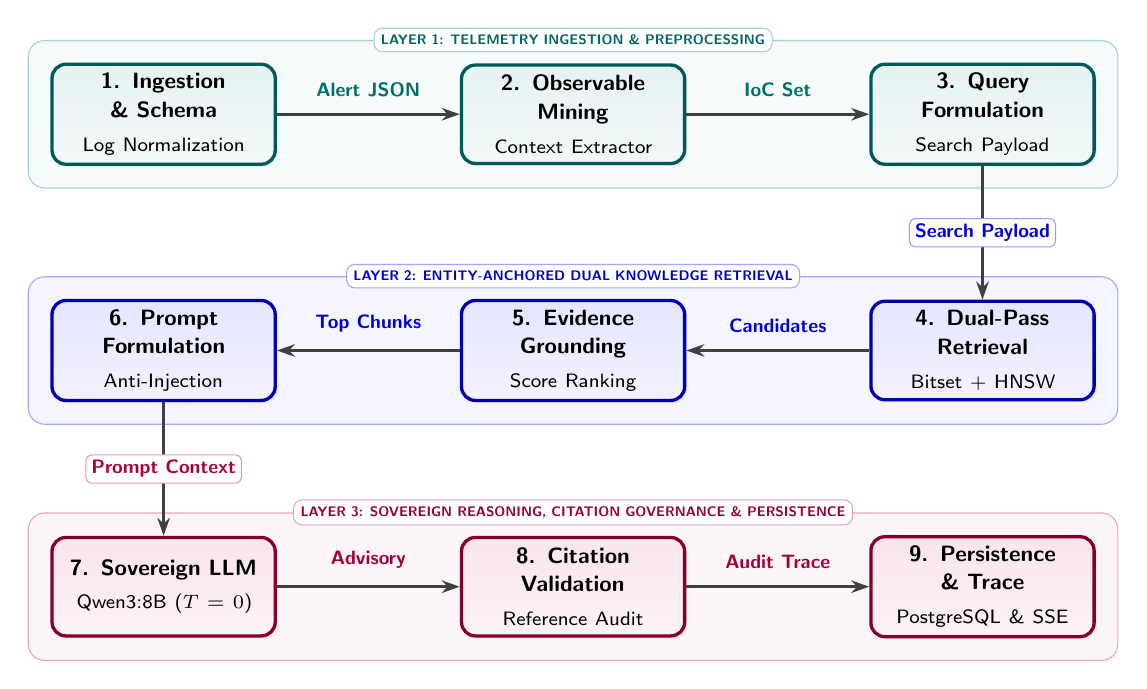
\begin{tikzpicture}[
    stage/.style={
        rectangle, rounded corners=5pt, draw=teal!70!black, top color=teal!10, bottom color=teal!5,
        very thick, text width=2.6cm, minimum height=1.25cm, align=center, font=\footnotesize\sffamily,
        drop shadow={opacity=0.10, shadow xshift=1pt, shadow yshift=-1pt},
        execute at begin node={\hyphenpenalty=10000\exhyphenpenalty=10000}
    },
    retrieval/.style={
        rectangle, rounded corners=5pt, draw=blue!70!black, top color=blue!10, bottom color=blue!5,
        very thick, text width=2.6cm, minimum height=1.25cm, align=center, font=\footnotesize\sffamily,
        drop shadow={opacity=0.10, shadow xshift=1pt, shadow yshift=-1pt},
        execute at begin node={\hyphenpenalty=10000\exhyphenpenalty=10000}
    },
    reasoning/.style={
        rectangle, rounded corners=5pt, draw=purple!70!black, top color=purple!10, bottom color=purple!5,
        very thick, text width=2.6cm, minimum height=1.25cm, align=center, font=\footnotesize\sffamily,
        drop shadow={opacity=0.10, shadow xshift=1pt, shadow yshift=-1pt},
        execute at begin node={\hyphenpenalty=10000\exhyphenpenalty=10000}
    },
    arrow/.style={-{Stealth[length=6.5pt, width=4.5pt]}, very thick, draw=black!75},
    lbl/.style={font=\scriptsize\bfseries\sffamily, above=3pt}
]

    % Row 1: Telemetry Ingestion (Left to Right)
    \node[stage] (s1) at (0, 0) {\textbf{1. Ingestion \& Schema}\\[2pt]\scriptsize Log Normalization};
    \node[stage] (s2) at (5.2, 0) {\textbf{2. Observable Mining}\\[2pt]\scriptsize Context Extractor};
    \node[stage] (s3) at (10.4, 0) {\textbf{3. Query Formulation}\\[2pt]\scriptsize Search Payload};

    % Row 2: Dual Knowledge Retrieval (Right to Left)
    \node[retrieval] (s4) at (10.4, -3.0) {\textbf{4. Dual-Pass Retrieval}\\[2pt]\scriptsize Bitset + HNSW};
    \node[retrieval] (s5) at (5.2, -3.0) {\textbf{5. Evidence Grounding}\\[2pt]\scriptsize Score Ranking};
    \node[retrieval] (s6) at (0, -3.0) {\textbf{6. Prompt Formulation}\\[2pt]\scriptsize Anti-Injection};

    % Row 3: Sovereign Inference & Governance (Left to Right)
    \node[reasoning] (s7) at (0, -6.0) {\textbf{7. Sovereign LLM}\\[2pt]\scriptsize Qwen3:8B ($T=0$)};
    \node[reasoning] (s8) at (5.2, -6.0) {\textbf{8. Citation Validation}\\[2pt]\scriptsize Reference Audit};
    \node[reasoning] (s9) at (10.4, -6.0) {\textbf{9. Persistence \& Trace}\\[2pt]\scriptsize PostgreSQL \& SSE};

    % Horizontal Connectors with generous margins (>5mm clearance on both sides)
    \draw[arrow] (s1.east) -- (s2.west);
    \node[lbl, color=teal!85!black] at ($(s1.east)!0.5!(s2.west)$) {Alert JSON};

    \draw[arrow] (s2.east) -- (s3.west);
    \node[lbl, color=teal!85!black] at ($(s2.east)!0.5!(s3.west)$) {IoC Set};

    \draw[arrow] (s4.west) -- (s5.east);
    \node[lbl, color=blue!85!black] at ($(s4.west)!0.5!(s5.east)$) {Candidates};

    \draw[arrow] (s5.west) -- (s6.east);
    \node[lbl, color=blue!85!black] at ($(s5.west)!0.5!(s6.east)$) {Top Chunks};

    \draw[arrow] (s7.east) -- (s8.west);
    \node[lbl, color=purple!85!black] at ($(s7.east)!0.5!(s8.west)$) {Advisory};

    \draw[arrow] (s8.east) -- (s9.west);
    \node[lbl, color=purple!85!black] at ($(s8.east)!0.5!(s9.west)$) {Audit Trace};

    % Vertical Connectors with pill badges centered in open gap
    \draw[arrow] (s3.south) -- (s4.north);
    \node[font=\scriptsize\bfseries\sffamily\color{blue!90!black}, fill=white, draw=blue!40, rounded corners=2pt, inner sep=2pt] at ($(s3.south)!0.5!(s4.north)$) {Search Payload};

    \draw[arrow] (s6.south) -- (s7.north);
    \node[font=\scriptsize\bfseries\sffamily\color{purple!90!black}, fill=white, draw=purple!40, rounded corners=2pt, inner sep=2pt] at ($(s6.south)!0.5!(s7.north)$) {Prompt Context};

    % Layer Background Bounding Boxes (inner ysep=6pt leaves 1.6cm open gap between rows)
    \begin{scope}[on background layer]
        \node[fill=teal!4, draw=teal!35, rounded corners=6pt, fit=(s1) (s3), inner xsep=8pt, inner ysep=8pt] (layer1) {};
        \node[fill=blue!4, draw=blue!35, rounded corners=6pt, fit=(s6) (s4), inner xsep=8pt, inner ysep=8pt] (layer2) {};
        \node[fill=purple!4, draw=purple!35, rounded corners=6pt, fit=(s7) (s9), inner xsep=8pt, inner ysep=8pt] (layer3) {};
    \end{scope}

    % Clean Layer Header Badges
    \node[font=\tiny\bfseries\sffamily\color{teal!80!black}, fill=white, draw=teal!35, rounded corners=3pt, inner sep=2.5pt] at (layer1.north) {LAYER 1: TELEMETRY INGESTION \& PREPROCESSING};
    \node[font=\tiny\bfseries\sffamily\color{blue!80!black}, fill=white, draw=blue!35, rounded corners=3pt, inner sep=2.5pt] at (layer2.north) {LAYER 2: ENTITY-ANCHORED DUAL KNOWLEDGE RETRIEVAL};
    \node[font=\tiny\bfseries\sffamily\color{purple!80!black}, fill=white, draw=purple!35, rounded corners=3pt, inner sep=2.5pt] at (layer3.north) {LAYER 3: SOVEREIGN REASONING, CITATION GOVERNANCE \& PERSISTENCE};

\end{tikzpicture}%
}
\caption{Algorithmic pipeline workflow of the AI-Powered SOC Assistant, illustrating the 9 sequential stages across Ingestion, Entity-Anchored Retrieval, and Citation-Governed Sovereign Reasoning.}
\label{fig:methodology_flow}
\end{figure}

\section{Alert Ingestion and Security Normalization}
\label{sec:impl_normalization}
When an alert is received, \texttt{AlertService} maps the incoming JSON or Syslog string into the canonical \texttt{NormalizedSecurityAlert} model:
\begin{itemize}
    \item Resolves timestamps into standardized UTC ISO-8601 strings.
    \item Cleans IPv4/IPv6 strings, stripping port numbers and whitespace.
    \item Maps numerical severities ($0 \le s \le 16$) to ratings (\texttt{LOW}, \texttt{MEDIUM}, \texttt{HIGH}, \texttt{CRITICAL}).
    \item Parses MITRE technique identifiers from Wazuh XML metadata (\texttt{rule.mitre.id}).
\end{itemize}

\section{Deterministic Security Context Extraction}
\label{sec:impl_context}
The second stage executes observable mining via \texttt{ContextExtractor}. Operating deterministically without probabilistic LLM calls, it structures:
\begin{enumerate}[itemsep=1pt,topsep=2pt]
    \item \textbf{Network Indicators:} Source and destination IP addresses and ports.
    \item \textbf{Host Attributes:} Usernames, agent hostnames, operating systems, and process binary paths.
    \item \textbf{Keyword Tokenization:} Tokenizes rule descriptions via regex, filtering against stop-words.
    \item \textbf{Attack Term Mining:} Matches tokens against a taxonomy of 38 attack signals (e.g., \texttt{brute}, \texttt{injection}, \texttt{ransomware}, \texttt{escalation}, \texttt{exfiltration}).
\end{enumerate}

\begin{lstlisting}[language=Python, caption={Deterministic keyword filtering in \texttt{ContextExtractor}.}]
def _keywords_from_text(text: Optional[str]) -> List[str]:
    if not text:
        return []
    tokens = [t.lower().strip(".:,;()[]") for t in _TOKEN_RE.findall(text)]
    return [t for t in tokens if t not in _STOP_WORDS
            and t not in _NOISE_TOKENS and len(t) >= 3]
\end{lstlisting}

\section{Categorized Retrieval Query Construction}
\label{sec:impl_query_builder}
Query compilation in \texttt{RetrievalQueryBuilder} synthesizes up to three distinct query categories:
\begin{enumerate}[itemsep=1pt,topsep=2pt]
    \item \textbf{MITRE Technique Queries:} Created if explicit technique IDs exist (e.g., $Q_{\text{mitre}} = \text{``MITRE ATT\&CK technique } T\text{''}$).
    \item \textbf{NVD / CVE Queries:} Synthesized on CVE regex matches ($Q_{\text{nvd}} = \text{``CVE details''}$).
    \item \textbf{General Security Queries:} Built from normalized event types and top descriptive keywords.
\end{enumerate}

\section{Offline Knowledge Ingestion and Chunking Pipeline}
\label{sec:impl_chunking}
Knowledge ingestion runs offline via \texttt{app/rag/ingest\_knowledge.py}:
\begin{itemize}[itemsep=1pt,topsep=2pt]
    \item \textbf{MITRE ATT\&CK Enterprise Matrix v14.1:} Parsed from STIX 2.1 JSON into 1,618 technique chunks.
    \item \textbf{NIST National Vulnerability Database (NVD):} Indexed into 144 structured CVE chunks.
\end{itemize}
Total indexed corpus size: \textbf{1,762 vector chunks}, embedded into 384-dimensional dense vectors using \texttt{all-MiniLM-\allowbreak L6-v2} alongside metadata payloads (\texttt{source\_id}, \texttt{tactics}, \texttt{title}).

\section{Dual-Pass Entity-Anchored Retrieval Formulation}
\label{sec:impl_retriever}
To eliminate semantic drift, \texttt{Retriever} executes a \textbf{dual-pass search}:
\begin{enumerate}[itemsep=1pt,topsep=2pt]
    \item \textbf{Pass 1 (Payload-Filtered):} For queries carrying MITRE or CVE IDs, Qdrant executes exact payload filtering matching the target identifier.
    \item \textbf{Pass 2 (Dense Semantic Search):} The query vector $\mathbf{v}_q$ is searched across the corpus using unconstrained cosine similarity.
    \item \textbf{Merging and Deduplication:} Results from both passes are merged, retaining the highest genuine cosine score per chunk.
\end{enumerate}

\begin{lstlisting}[language=Python, caption={Dual-pass hybrid search implementation in \texttt{app/rag/retriever.py}.}]
for payload_filter in search_passes:
    pass_results = self._index.search(
        query_vector=vector, top_k=top_k, payload_filter=payload_filter
    )
    for res in pass_results:
        cid = res.chunk_id
        if cid not in accumulated:
            accumulated[cid] = {"chunk": res, "best_score": res.similarity_score}
        elif res.similarity_score > accumulated[cid]["best_score"]:
            accumulated[cid]["best_score"] = res.similarity_score
\end{lstlisting}

\section{Tri-Mode Analysis Execution Paradigms}
\label{sec:impl_tri_mode}
To scientifically evaluate retrieval impact, the orchestrator implements three operational modes:
\begin{enumerate}
    \item \textbf{Mode 1: LLM-Only (\texttt{llm\_only}):} Retrieval is bypassed. The raw alert JSON is evaluated directly by Qwen3:8B, measuring pure parametric pre-training memorization.
    \item \textbf{Mode 2: Standard RAG (\texttt{standard\_rag}):} Unanchored dense cosine similarity over the alert description; top-5 nearest chunks are injected into context.
    \item \textbf{Mode 3: Evidence-Aware RAG (\texttt{evidence\_aware}):} Our contribution: observables are extracted, dual-pass retrieval executes, and citation validation is enforced.
\end{enumerate}

\section{Prompt Formulation and Anti-Injection Constraints}
\label{sec:impl_prompts}
The orchestrator compiles a system prompt enforcing defensive constraints and structured JSON:
\begin{lstlisting}[caption={Standardized JSON output schema required from the LLM.}]
{
  "summary": "1-2 sentence executive summary",
  "severity_assessment": "Technical rationale for assigned severity",
  "observed_indicators": ["192.168.1.105", "admin", "T1110"],
  "suspected_techniques": ["T1110.001"],
  "reasoning": "Detailed forensic explanation",
  "investigation_steps": ["Check auth logs", "Review firewall"],
  "confidence": "HIGH", "limitations": "Missing packet capture",
  "evidence_references": [{"evidence_id": "Exact matching ID", "claim": "...", "supporting_text": "..."}]
}
\end{lstlisting}
Rules mandate: (1) NEVER invent evidence IDs; (2) State missing evidence in limitations; (3) All investigation steps must be non-destructive; (4) Distinguish facts from hypotheses.

\section{Automated Citation Reference Validation Engine}
\label{sec:impl_citation_validator}
To eliminate generative hallucinations, \texttt{\_validate\_evidence()} parses the generated JSON and cross-examines citations against the actually retrieved evidence dictionary:
\begin{itemize}
    \item \textbf{Reference Existence Check:} Valid citation IDs are stored in PostgreSQL with relevance scores.
    \item \textbf{Hallucination Trapping:} Invented IDs are stripped from official evidence, and an explicit warning is appended to limitations: \texttt{Note: LLM hallucinated unknown evidence reference 'X'}.
\end{itemize}

\begin{lstlisting}[language=Python, caption={Citation validation and hallucination trapping in \texttt{orchestrator.py}.}]
def _validate_evidence(self, analysis: SOCAnalysis, evidence_set: Optional[EvidenceSet]):
    valid_dict = {ev.evidence_id: ev for ev in evidence_set.evidence} if evidence_set else {}
    validated_refs, evidence_creates = [], []
    for ref in analysis.evidence_references:
        if ref.evidence_id in valid_dict:
            validated_refs.append(ref)
            ev = valid_dict[ref.evidence_id]
            evidence_creates.append(EvidenceCreate(
                source=ev.source, title=ev.title, relevance_score=ev.similarity_score,
                citation=f"{ev.source_identifier} - {ev.title}"
            ))
        else:
            analysis.limitations += f"\nNote: LLM hallucinated unknown reference '{ref.evidence_id}'."
    return validated_analysis, evidence_creates
\end{lstlisting}

\section{Analyst User Interface and Interactive Entity Graph}
\label{sec:impl_frontend}
The presentation layer is a React 19 single-page console built with TypeScript and Tailwind CSS:
\begin{itemize}
    \item \textbf{Live Triage Queue:} Ingestion queue with severity badges, technique tags, and source filters.
    \item \textbf{D3.js Entity Graph:} Force-directed canvas displaying relationships between alerts, IPs, users, and MITRE techniques.
    \item \textbf{Real-Time Trace Waterfall:} Visualizes pipeline execution streaming over SSE with stage timings.
    \item \textbf{Technical Inspector Drawer:} Displays raw JSON payloads, cosine scores, and citation provenance.
\end{itemize}
%==============================================================================
% Chapter 6: Dataset Curation and Experimental Setup
%==============================================================================
\chapter{Dataset Curation and Experimental Setup}
\label{ch:experiments}
\label{chap:dataset_experiments}

\section{Dataset Design Principles and Research Provenance}
\label{sec:dataset_design}
Empirical evaluation of an AI-assisted SOC platform requires a benchmark reflecting operational enterprise complexity rather than toy queries. Real-world alerts contain dense JSON payloads, process paths, OS noise, and living-off-the-land commands. We curated \textbf{Dataset v2} (\texttt{backend/evaluation/dataset\_v2.json}) adhering to four core principles:
\begin{enumerate}
    \item \textbf{Tactical Completeness:} Scenarios span the complete cyber kill chain, from reconnaissance to data exfiltration.
    \item \textbf{Negative Control Representation:} Incorporates benign administrative tasks to evaluate false-alarm suppression.
    \item \textbf{Authoritative Ground Truth:} Mapped to MITRE ATT\&CK technique IDs and NIST NVD CVE records.
    \item \textbf{Input Isolation:} Ground-truth tags are withheld from the model; only raw alert observables are provided.
\end{enumerate}

\section{Evolution from Dataset v1 to Dataset v2 and Data Integrity Fixes}
\label{sec:dataset_evolution}
During Stage 1 auditing, a critical data integrity defect was uncovered in the initial setup:
\begin{quote}
\itshape
\textbf{The Milestone 1 Alert ID Collision Bug:} The evaluation harness reused historical database primary keys (\texttt{alert\_id} 1 to 40) across successive runs, causing Dataset v2 runs to inadvertently link to historical Dataset v1 payloads, distorting evaluation metrics.
\end{quote}
To resolve this defect and establish complete experimental integrity:
\begin{itemize}
    \item \textbf{Alembic Migration \texttt{c01\_datasource}:} Added an indexed \texttt{data\_source} column, strictly isolating \texttt{replay\_v2} records from interactive \texttt{demo} and \texttt{wazuh\_live} alerts.
    \item \textbf{Strict Identifier Namespacing:} Scenarios were namespaced as \texttt{v2-eval-001} through \texttt{v2-eval-040}.
    \item \textbf{Dedicated Test Suite:} Six automated integrity tests verify zero collisions and idempotent seeding.
\end{itemize}

\section{Dataset Composition and Category Distribution}
\label{sec:dataset_composition}
Dataset v2 comprises \textbf{40 curated, non-overlapping enterprise scenarios} structured across \textbf{10 uniform tactical categories} with exactly $N = 4$ scenarios each ($10 \times 4 = 40$ cases), summarized in Table \ref{tab:dataset_distribution}.

\begin{table}[!htbp]
\centering
\caption{Dataset v2 composition and scenario category distribution.}
\label{tab:dataset_distribution}
\small
\begin{tabularx}{\textwidth}{@{}l l c X@{}}
\toprule
\textbf{Category ID} & \textbf{Tactical Category} & \textbf{Count ($N$)} & \textbf{Representative Attack Scenarios / Activities} \\
\midrule
Cat-01 & Reconnaissance & 4 & Nmap SYN scan, active directory user enum, ping sweep. \\
Cat-02 & Initial Access & 4 & Spearphishing doc, external RDP probe, web shell upload. \\
Cat-03 & Execution & 4 & Encoded PowerShell script, CMD execution, WMI invocation. \\
Cat-04 & Persistence & 4 & Scheduled task creation, registry Run key, service install. \\
Cat-05 & Privilege Escalation & 4 & Sudo abuse, UAC bypass, token impersonation, setuid binary. \\
Cat-06 & Defense Evasion & 4 & Event log wipe, process injection, masquerading in Temp. \\
Cat-07 & Credential Access & 4 & LSASS memory dump, SSH brute force, /etc/shadow read. \\
Cat-08 & Command and Control & 4 & Outbound RDP session, DNS tunneling, HTTPS beaconing. \\
Cat-09 & Impact & 4 & Ransomware note drop, file encryption, database wipe. \\
Cat-10 & Benign Negative Controls & 4 & Authorized Nessus scan, sysadmin backup, PowerShell update. \\
\midrule
\textbf{Total} & \textbf{10 Uniform Categories} & \textbf{40} & \textbf{36 Multi-Stage Attack Cases + 4 Benign Controls} \\
\bottomrule
\end{tabularx}
\end{table}

\section{Experimental Execution Protocol}
\label{sec:experimental_protocol}
Benchmark evaluation was conducted using \texttt{backend/scripts/run\_evaluation.py} under strict controls:
\begin{enumerate}
    \item \textbf{Tri-Mode Space:} $40 \text{ Scenarios} \times 3 \text{ Modes} = \mathbf{120} \text{ Full Pipeline Evaluations}$.
    \item \textbf{Zero Runtime Errors:} All 120 runs completed to 100\% execution without exceptions (run ID \texttt{20261109-185423-0f4cfd}).
    \item \textbf{Deterministic Inference:} Qwen3:8B executed at $T = 0.0$ and \texttt{top\_p} = 1.0 for reproducible evaluation.
    \item \textbf{Artifact Preservation:} Full capture of prompts, tokens, vector scores, and nanosecond timings.
\end{enumerate}

\section{Isolated Retrieval Ablation Protocol}
\label{sec:ablation_protocol}
A critical methodological distinction enforced in this work is separating retrieval evaluation from generation. Generation quirks can mask retrieval efficacy. We executed an isolated, headless \textbf{Retrieval Ablation} across all 40 scenarios against 1,762 vector chunks without an LLM:
\begin{itemize}
    \item Evaluated three retrieval configurations: Standard RAG (unanchored dense cosine), Evidence-Aware RAG (entity-anchored hybrid), and Token Hashing Baseline (offline lexical 2-gram hashing).
    \item Evaluated candidate rankings at top-$k \in \{1, 5, 10\}$, computing Recall@1, Recall@5, MRR, and latency.
\end{itemize}

\section{Hardware and Host Execution Parameters}
\label{sec:host_parameters}
All 120 benchmark runs and 40 ablation runs executed locally under the configuration in Table \ref{tab:execution_parameters}.

\begin{table}[!htbp]
\centering
\caption{Host experimental parameters and software configuration.}
\label{tab:execution_parameters}
\small
\begin{tabularx}{\textwidth}{@{}l p{4.2cm} X@{}}
\toprule
\textbf{Category} & \textbf{Component} & \textbf{Configuration Value / Version} \\
\midrule
\textbf{Host Hardware} & Processor (CPU) & Intel Core i7-12700H (14 cores, 20 threads) \\
                       & System Memory (RAM) & 32 GB DDR5 4800 MHz \\
                       & Storage Subsystem & 1 TB NVMe PCIe 4.0 SSD \\
                       & Graphics Accelerator & NVIDIA GeForce RTX 3060 Laptop GPU (6 GB VRAM) \\
\midrule
\textbf{Environment}   & Operating System & Windows 11 Pro 64-bit / WSL2 Ubuntu 22.04 \\
                       & Container Engine & Docker Desktop 4.79.0 / Docker Engine 29.5.3 \\
                       & Database Version & PostgreSQL 15.4 (Alpine container) \\
                       & Vector Engine & Qdrant v1.18.2 (Official container) \\
\midrule
\textbf{Model Config}  & Reasoning Model & Qwen3:8B (\texttt{qwen3:8b} via Ollama v0.5.4) \\
                       & Embedding Model & \texttt{sentence-transformers/\allowbreak all-MiniLM-L6-v2} (384-dim) \\
                       & Lexical Baseline & HashingEmbeddingProvider (2-gram, 256-dim) \\
                       & Decoding Temperature & $T = 0.0$ (Strict greedy decoding) \\
                       & Context Window & 32,768 tokens (Prompt truncated at 1,000 completion tokens) \\
\bottomrule
\end{tabularx}
\end{table}
%==============================================================================
% Chapter 7: Results and Performance Evaluation
%==============================================================================
\chapter{Results and Performance Evaluation}
\label{chap:results_evaluation}

This chapter presents the empirical findings and comprehensive evaluation of the AI-powered Security Operations Center (SOC) Assistant along two complementary axes:
\begin{enumerate}
    \item \textbf{End-to-End SOC Triage Performance:} A 120-run benchmark across 40 enterprise scenarios evaluated under \texttt{llm\_only}, \texttt{standard\_rag}, and \texttt{evidence\_aware} modes, assessing MITRE ATT\&CK classification, triage latency, benign control discrimination, and CVE identification.
    \item \textbf{Headless Knowledge Retrieval Ablation:} An isolated retrieval evaluation over 1,762 authoritative security chunks (MITRE ATT\&CK v14.1 and NIST NVD), measuring retrieval precision without language model generation in the loop.
\end{enumerate}

\section{MITRE ATT\&CK Technique Classification Performance}
\label{sec:mitre_classification_results}
Tier-1 triage requires accurately mapping raw telemetry to MITRE ATT\&CK techniques. Table \ref{tab:mitre_classification_metrics} summarizes performance across the 36 attack scenarios containing 54 ground-truth technique instances.

\begin{table}[!htbp]
\centering
\caption{MITRE ATT\&CK technique classification performance across 36 attack scenarios (54 target technique instances).}
\label{tab:mitre_classification_metrics}
\small
\begin{tabularx}{\textwidth}{@{}l c c c c c c c@{}}
\toprule
\textbf{Operational Mode} & \textbf{Precision} & \textbf{Recall} & \textbf{Macro F1} & \textbf{Micro F1} & \textbf{TP} & \textbf{FP} & \textbf{FN} \\
\midrule
\texttt{llm\_only}       & \textbf{0.9861} & \textbf{0.8611} & \textbf{0.9028} & \textbf{0.8889} & \textbf{44} & \textbf{1} & \textbf{10} \\
\texttt{standard\_rag}   & 0.9583          & 0.8333          & 0.8750          & 0.8776          & 43          & \textbf{1} & 11          \\
\texttt{evidence\_aware} & 0.9398          & 0.8333          & 0.8611          & 0.8600          & 43          & 3          & 11          \\
\bottomrule
\end{tabularx}
\end{table}

\begin{figure}[!htbp]
\centering
\centerline{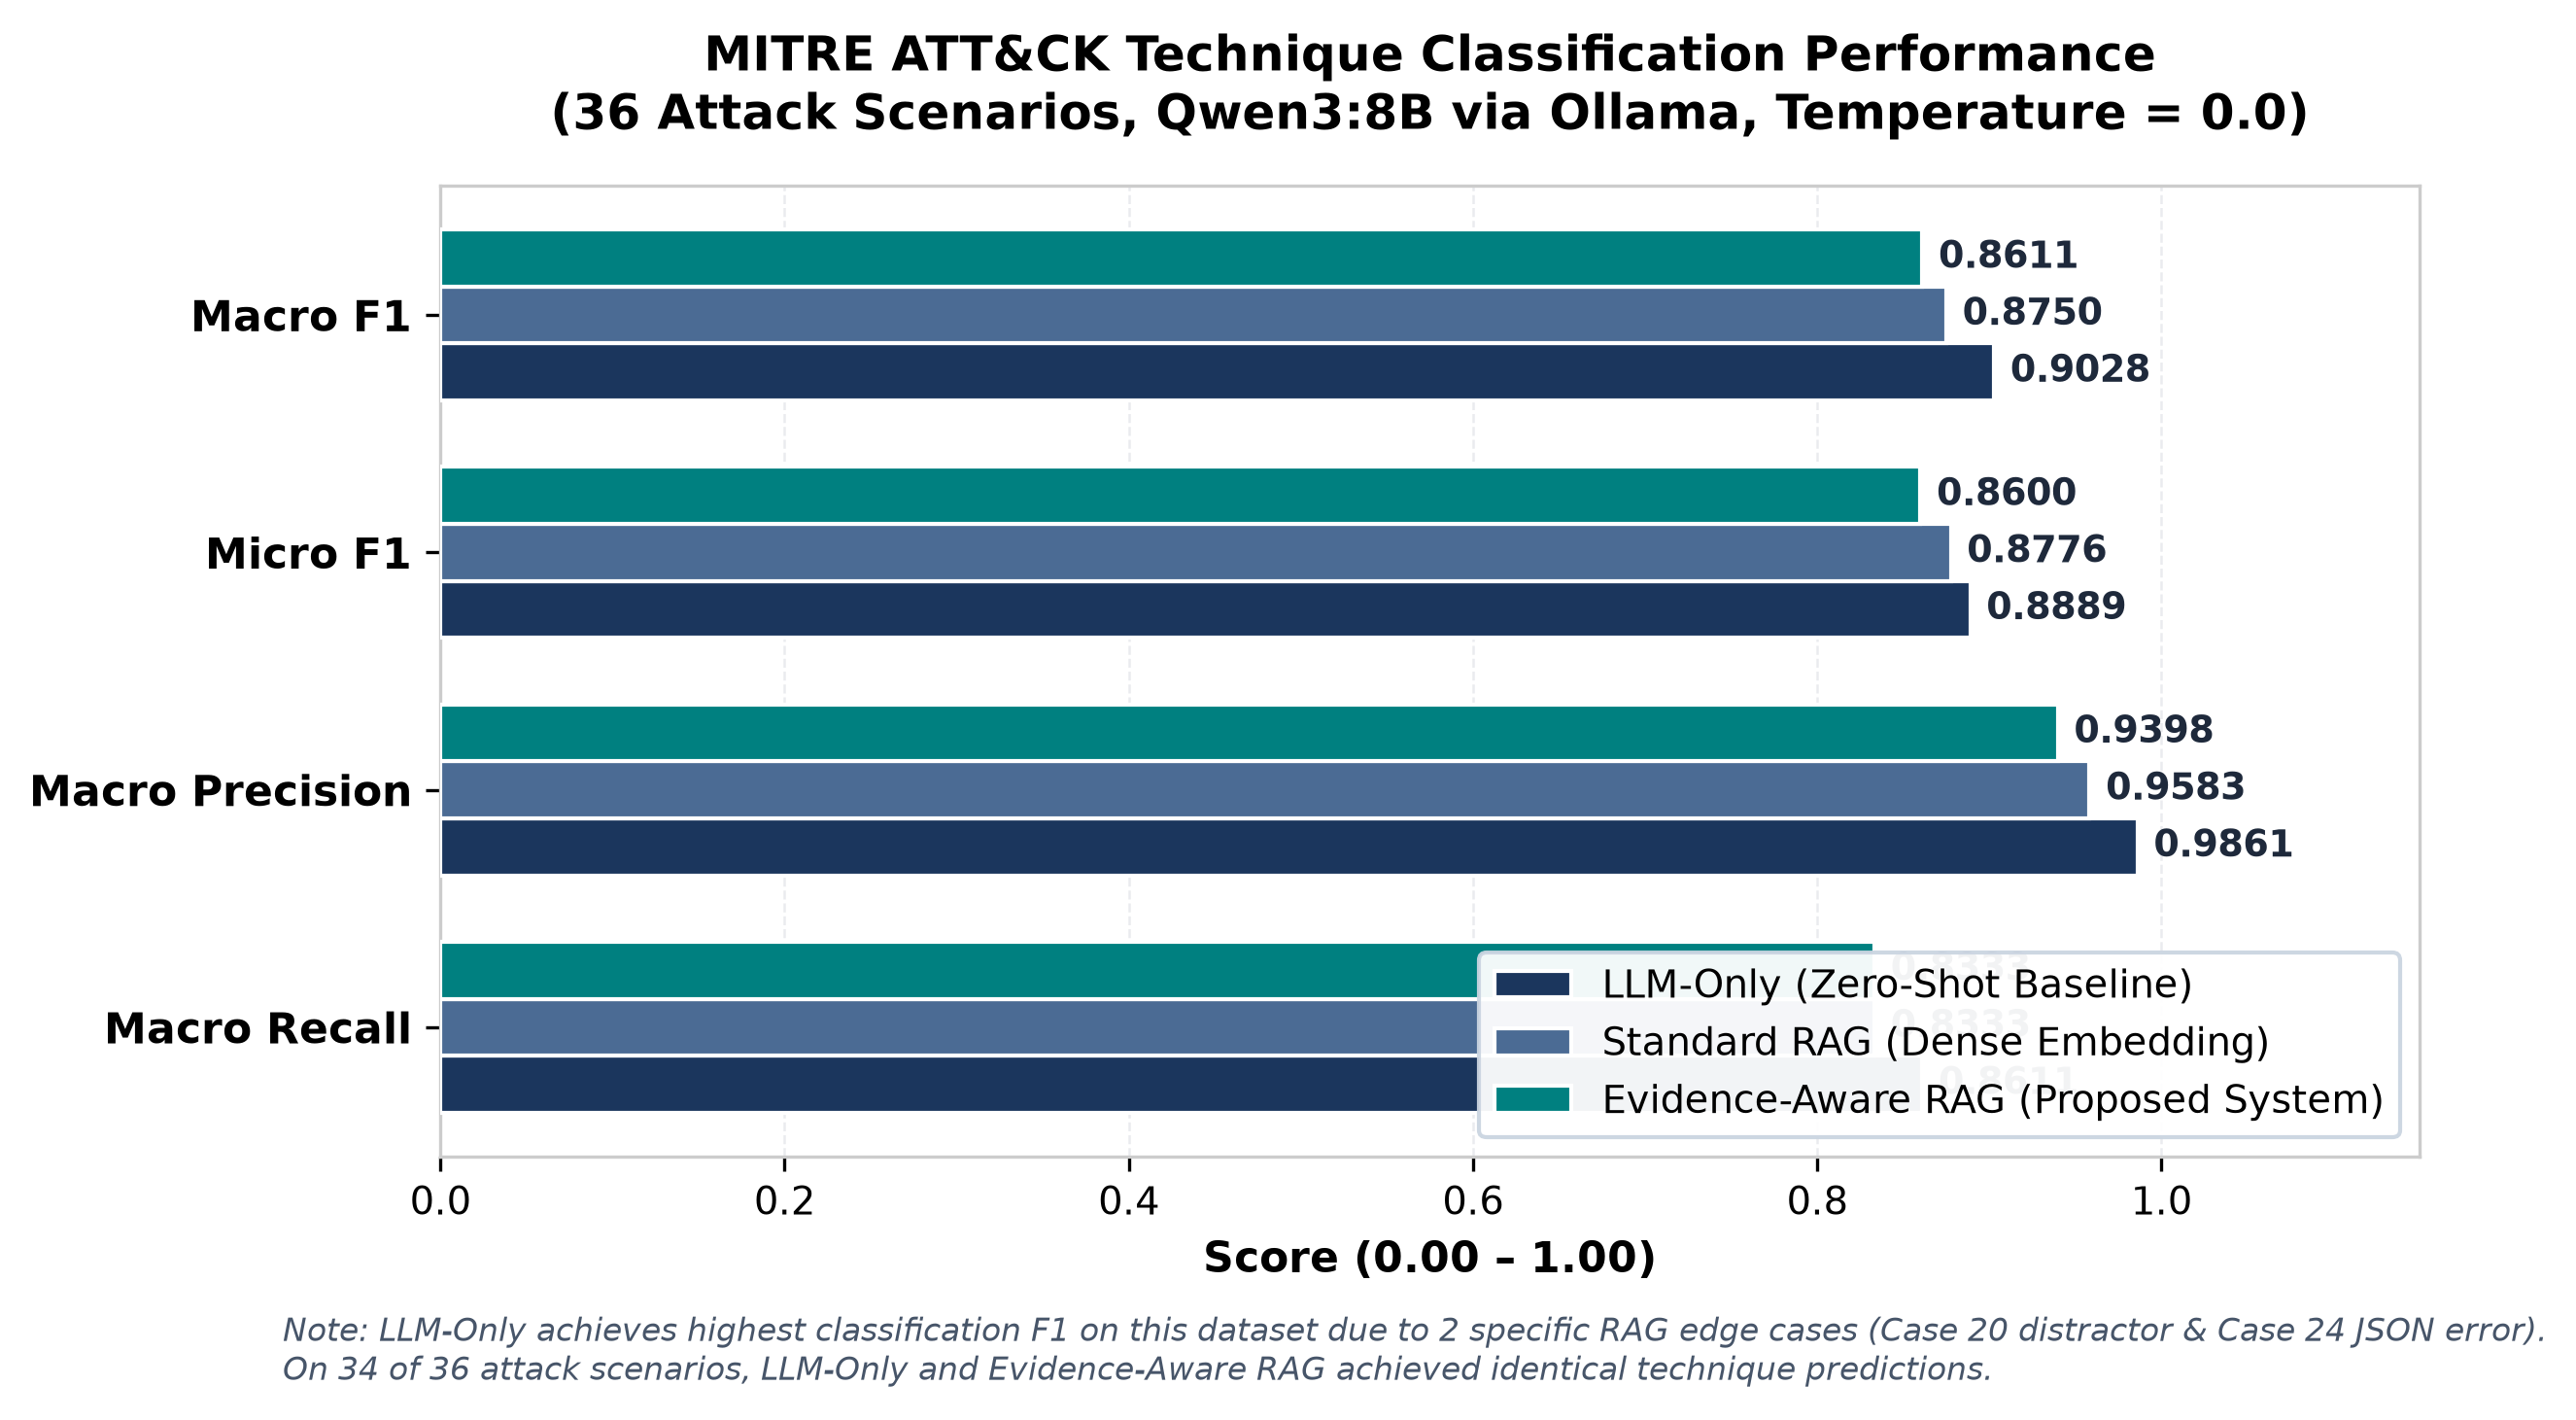
\includegraphics[width=1.04\textwidth]{figures/figure1_classification.png}}\vspace{4pt}
{\small (a) Multi-metric MITRE ATT\&CK technique classification comparison (Precision, Recall, Macro F1, Micro F1).}\vspace{12pt}
\centerline{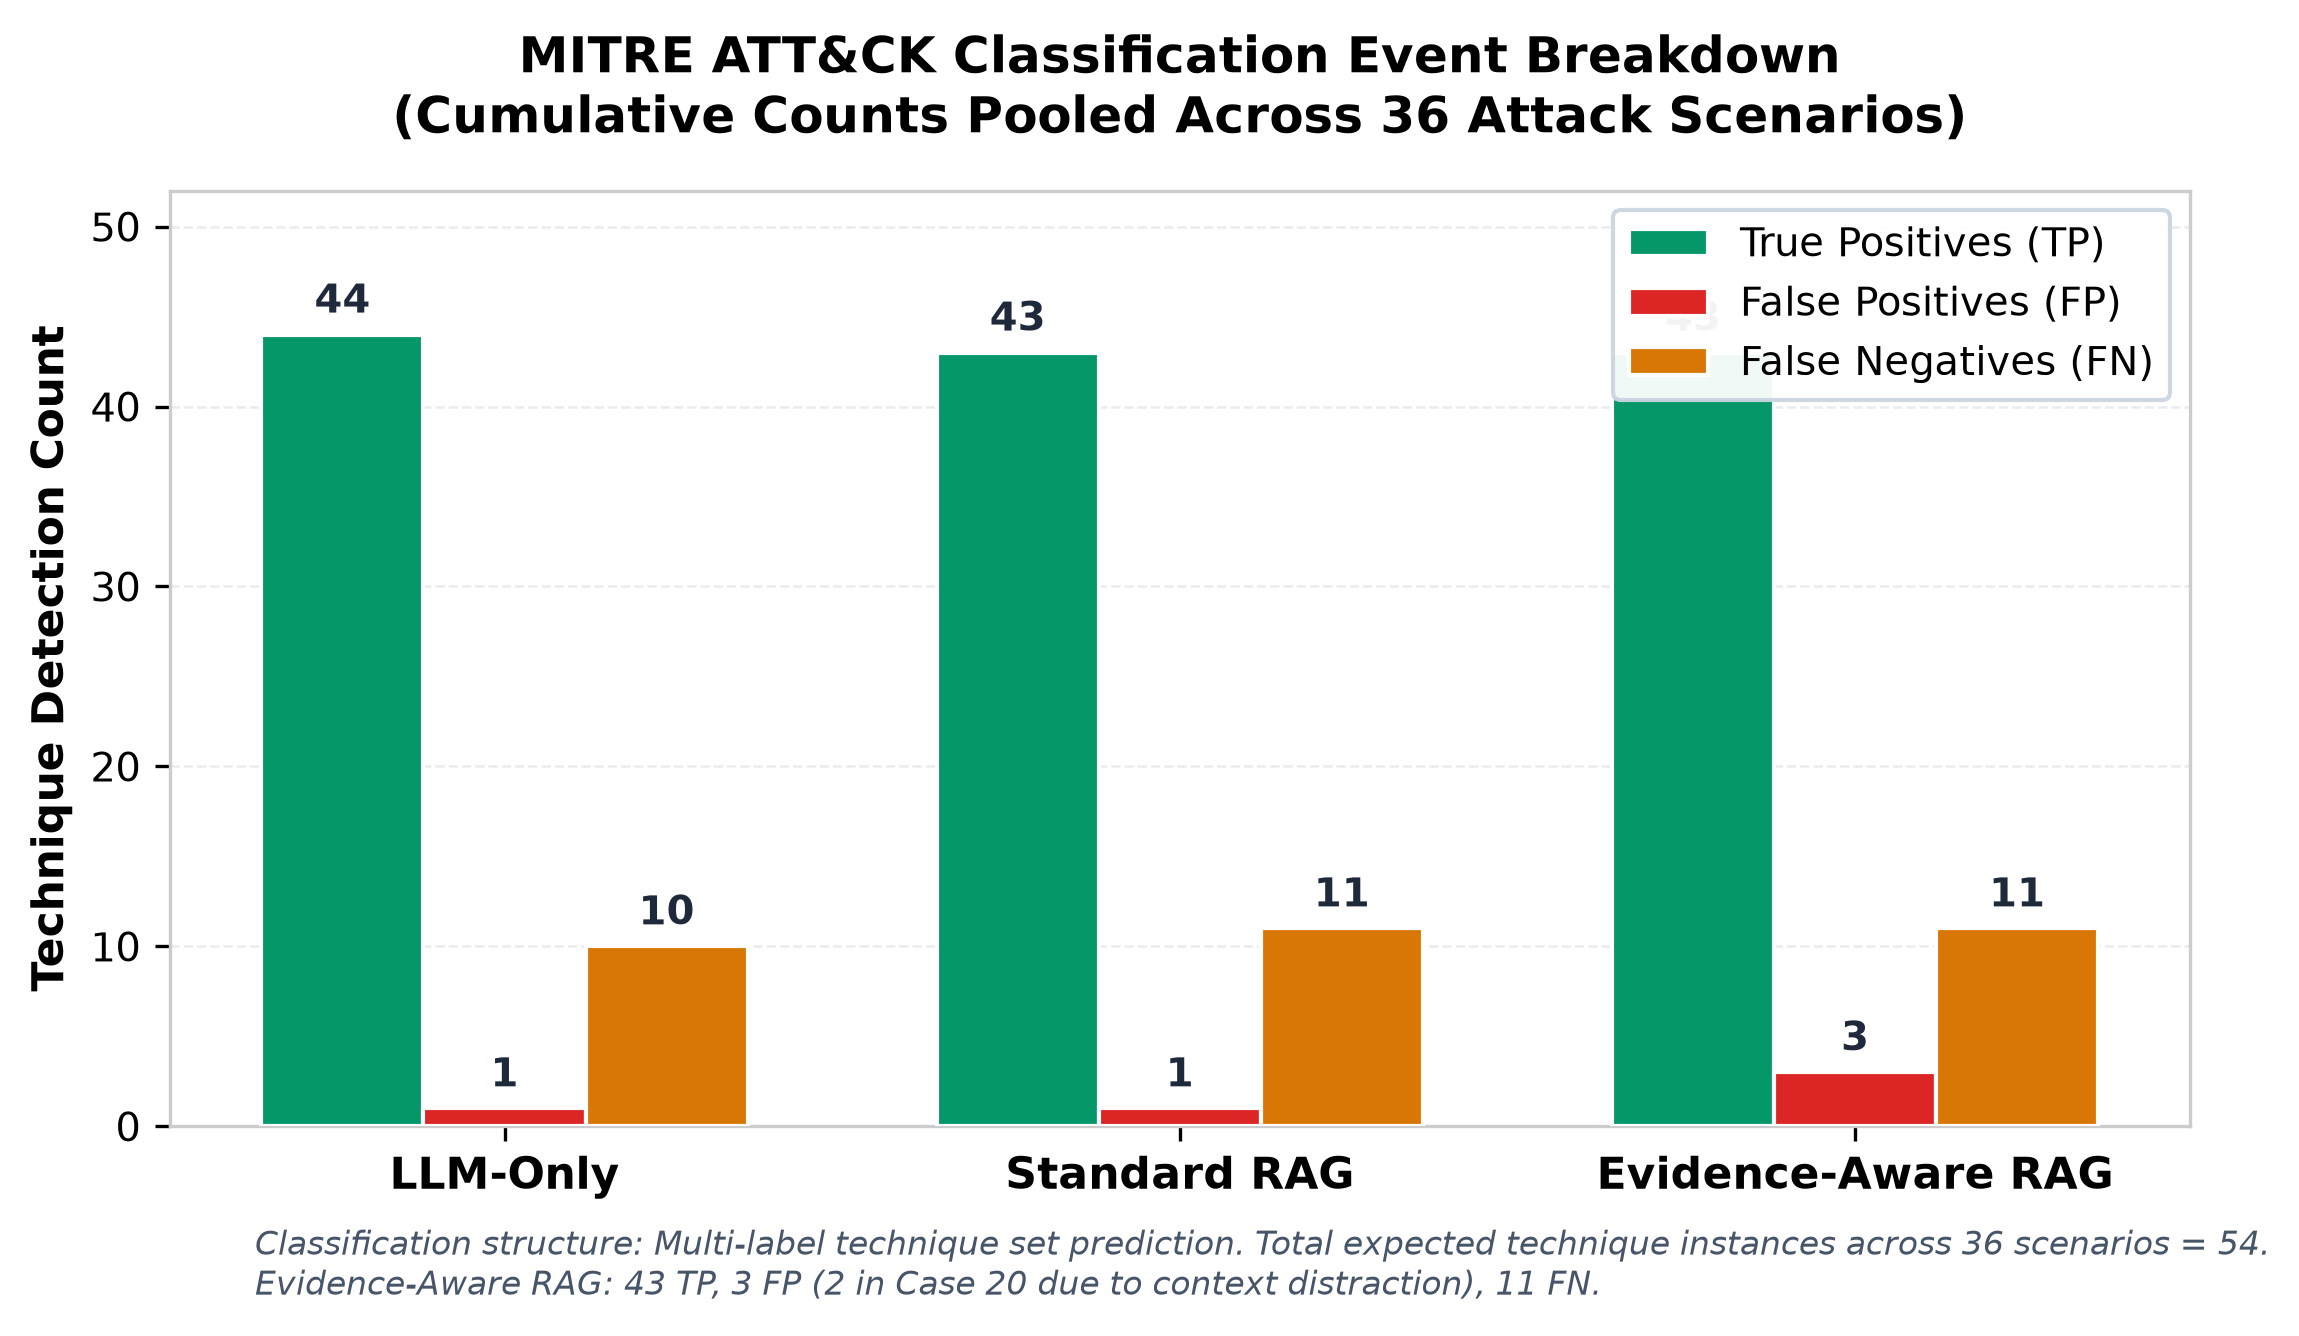
\includegraphics[width=1.0\textwidth]{figures/figure1_confusion_counts.png}}\vspace{4pt}
{\small (b) Underlying confusion counts (True Positives, False Positives, False Negatives).}
\caption{MITRE ATT\&CK technique classification performance across operational modes (36 attack scenarios, 54 target technique instances).}
\label{fig:mitre_classification_eval}
\end{figure}

\subsection{Deep-Dive Analysis of the F1 Discrepancy}
\label{subsec:f1_discrepancy_analysis}
Intellectual honesty requires examining why unaugmented \texttt{llm\_only} achieved a higher Macro F1 ($0.9028$) and Micro F1 ($0.8889$) than RAG modes. Granular case auditing revealed that:
\begin{enumerate}
    \item On \textbf{34 out of 36 attack scenarios (94.4\%)}, all three modes yielded \textbf{completely identical technique predictions}.
    \item The entire F1 performance gap is governed by exactly \textbf{two anomaly scenarios} (Table \ref{tab:failure_case_breakdown}):
    \begin{itemize}
        \item \textbf{Case 20 (\texttt{new-system-service}):} Ground truth is \texttt{T1543.003}. Under \texttt{llm\_only}, the model predicted \texttt{T1543.003} alone (F1 = 1.0). Under \texttt{evidence\_aware}, retrieved STIX chunks referenced adjacent techniques (\texttt{T1036} Masquerading and legacy \texttt{T1050}). Swayed by this rich context, the model predicted all three, inducing 2 False Positives (F1 = 0.50). This illustrates the \textbf{Context Distractor Effect}, where peripheral background text leads smaller parameter models (8B) to over-generate.
        \item \textbf{Case 24 (\texttt{unusual-outbound-rdp}):} Ground truth is \texttt{T1021.001}. Under \texttt{llm\_only} and \texttt{standard\_rag}, the model output valid JSON (F1 = 1.0). Under \texttt{evidence\_aware}, Qwen3:8B produced a minor Markdown delimiter glitch. The backend parser caught the syntax error and safely triggered the fallback parser, preserving summary and severity but returning an empty technique list to prevent schema corruption (F1 = 0.0).
    \end{itemize}
\end{enumerate}

\begin{table}[!htbp]
\centering
\caption{Detailed diagnostic breakdown of the two failure cases governing the F1 disparity.}
\label{tab:failure_case_breakdown}
\footnotesize
\setlength{\tabcolsep}{3.5pt}
\begin{tabularx}{\textwidth}{@{}l p{2.6cm} l X c c@{}}
\toprule
\textbf{Scenario ID} & \textbf{Scenario Name} & \textbf{Mode} & \textbf{Predicted Techniques} & \textbf{TP/FP/FN} & \textbf{F1} \\
\midrule
\multirow{2}{*}{\texttt{v2-eval-020}} & \texttt{new-system-} & \texttt{llm\_only} & \texttt{T1543.003} & 1 / 0 / 0 & \textbf{1.00} \\
    & \texttt{service} & \texttt{evidence\_aware} & \texttt{T1543.003, T1036, T1050} & 1 / 2 / 0 & 0.50 \\
\midrule
\multirow{2}{*}{\texttt{v2-eval-024}} & \texttt{unusual-} & \texttt{llm\_only} & \texttt{T1021.001} & 1 / 0 / 0 & \textbf{1.00} \\
    & \texttt{outbound-rdp} & \texttt{evidence\_aware} & None (Fallback Triggered) & 0 / 0 / 1 & 0.00 \\
\bottomrule
\end{tabularx}
\end{table}

\section{Knowledge Retrieval Ablation: Entity Anchoring vs Dense Search}
\label{sec:retrieval_ablation_results}
To evaluate retrieval without generation noise, we executed an isolated ablation across all 40 scenarios against 1,762 security chunks comparing Standard RAG (unanchored dense cosine), Evidence-Aware RAG (entity-anchored hybrid), and Token Hashing (lexical 2-gram hashing).

\begin{table}[!htbp]
\centering
\caption{Headless knowledge retrieval ablation results across 40 evaluation scenarios against 1,762 indexed security chunks.}
\label{tab:retrieval_ablation_metrics}
\footnotesize
\setlength{\tabcolsep}{4.5pt}
\begin{tabularx}{\textwidth}{@{}X c c c c@{}}
\toprule
\textbf{Retrieval Configuration} & \textbf{Recall@1} & \textbf{Recall@5} & \textbf{MRR} & \textbf{Mean Latency (ms)} \\
\midrule
\texttt{standard\_rag} (Unanchored Dense) & 22.5\% (9/40) & 40.0\% (16/40) & 0.2742 & 51.5 $\pm$ 4.8 \\
\texttt{evidence\_aware} (Entity-Anchored) & \textbf{90.0\%} (36/40) & \textbf{92.5\%} (37/40) & \textbf{0.9125} & 240.2 $\pm$ 18.6 \\
\texttt{hashing} (Lexical 2-Gram Baseline) & \textbf{92.5\%} (37/40) & \textbf{92.5\%} (37/40) & \textbf{0.9250} & \textbf{38.9} $\pm$ 3.2 \\
\bottomrule
\end{tabularx}
\end{table}

\subsection{The Breakthrough: Why Entity Anchoring Dominates Dense Search}
\label{subsec:anchoring_breakthrough}
Table \ref{tab:retrieval_ablation_metrics} demonstrates a breakthrough: \textbf{Evidence-Aware RAG improves Recall@1 from 22.5\% to 90.0\%---an absolute surge of 67.5 percentage points} over Standard RAG, while MRR jumps from $0.2742$ to $0.9125$ (Figure \ref{fig:retrieval_ablation_eval}).

\begin{figure}[!htbp]
\centering
\centerline{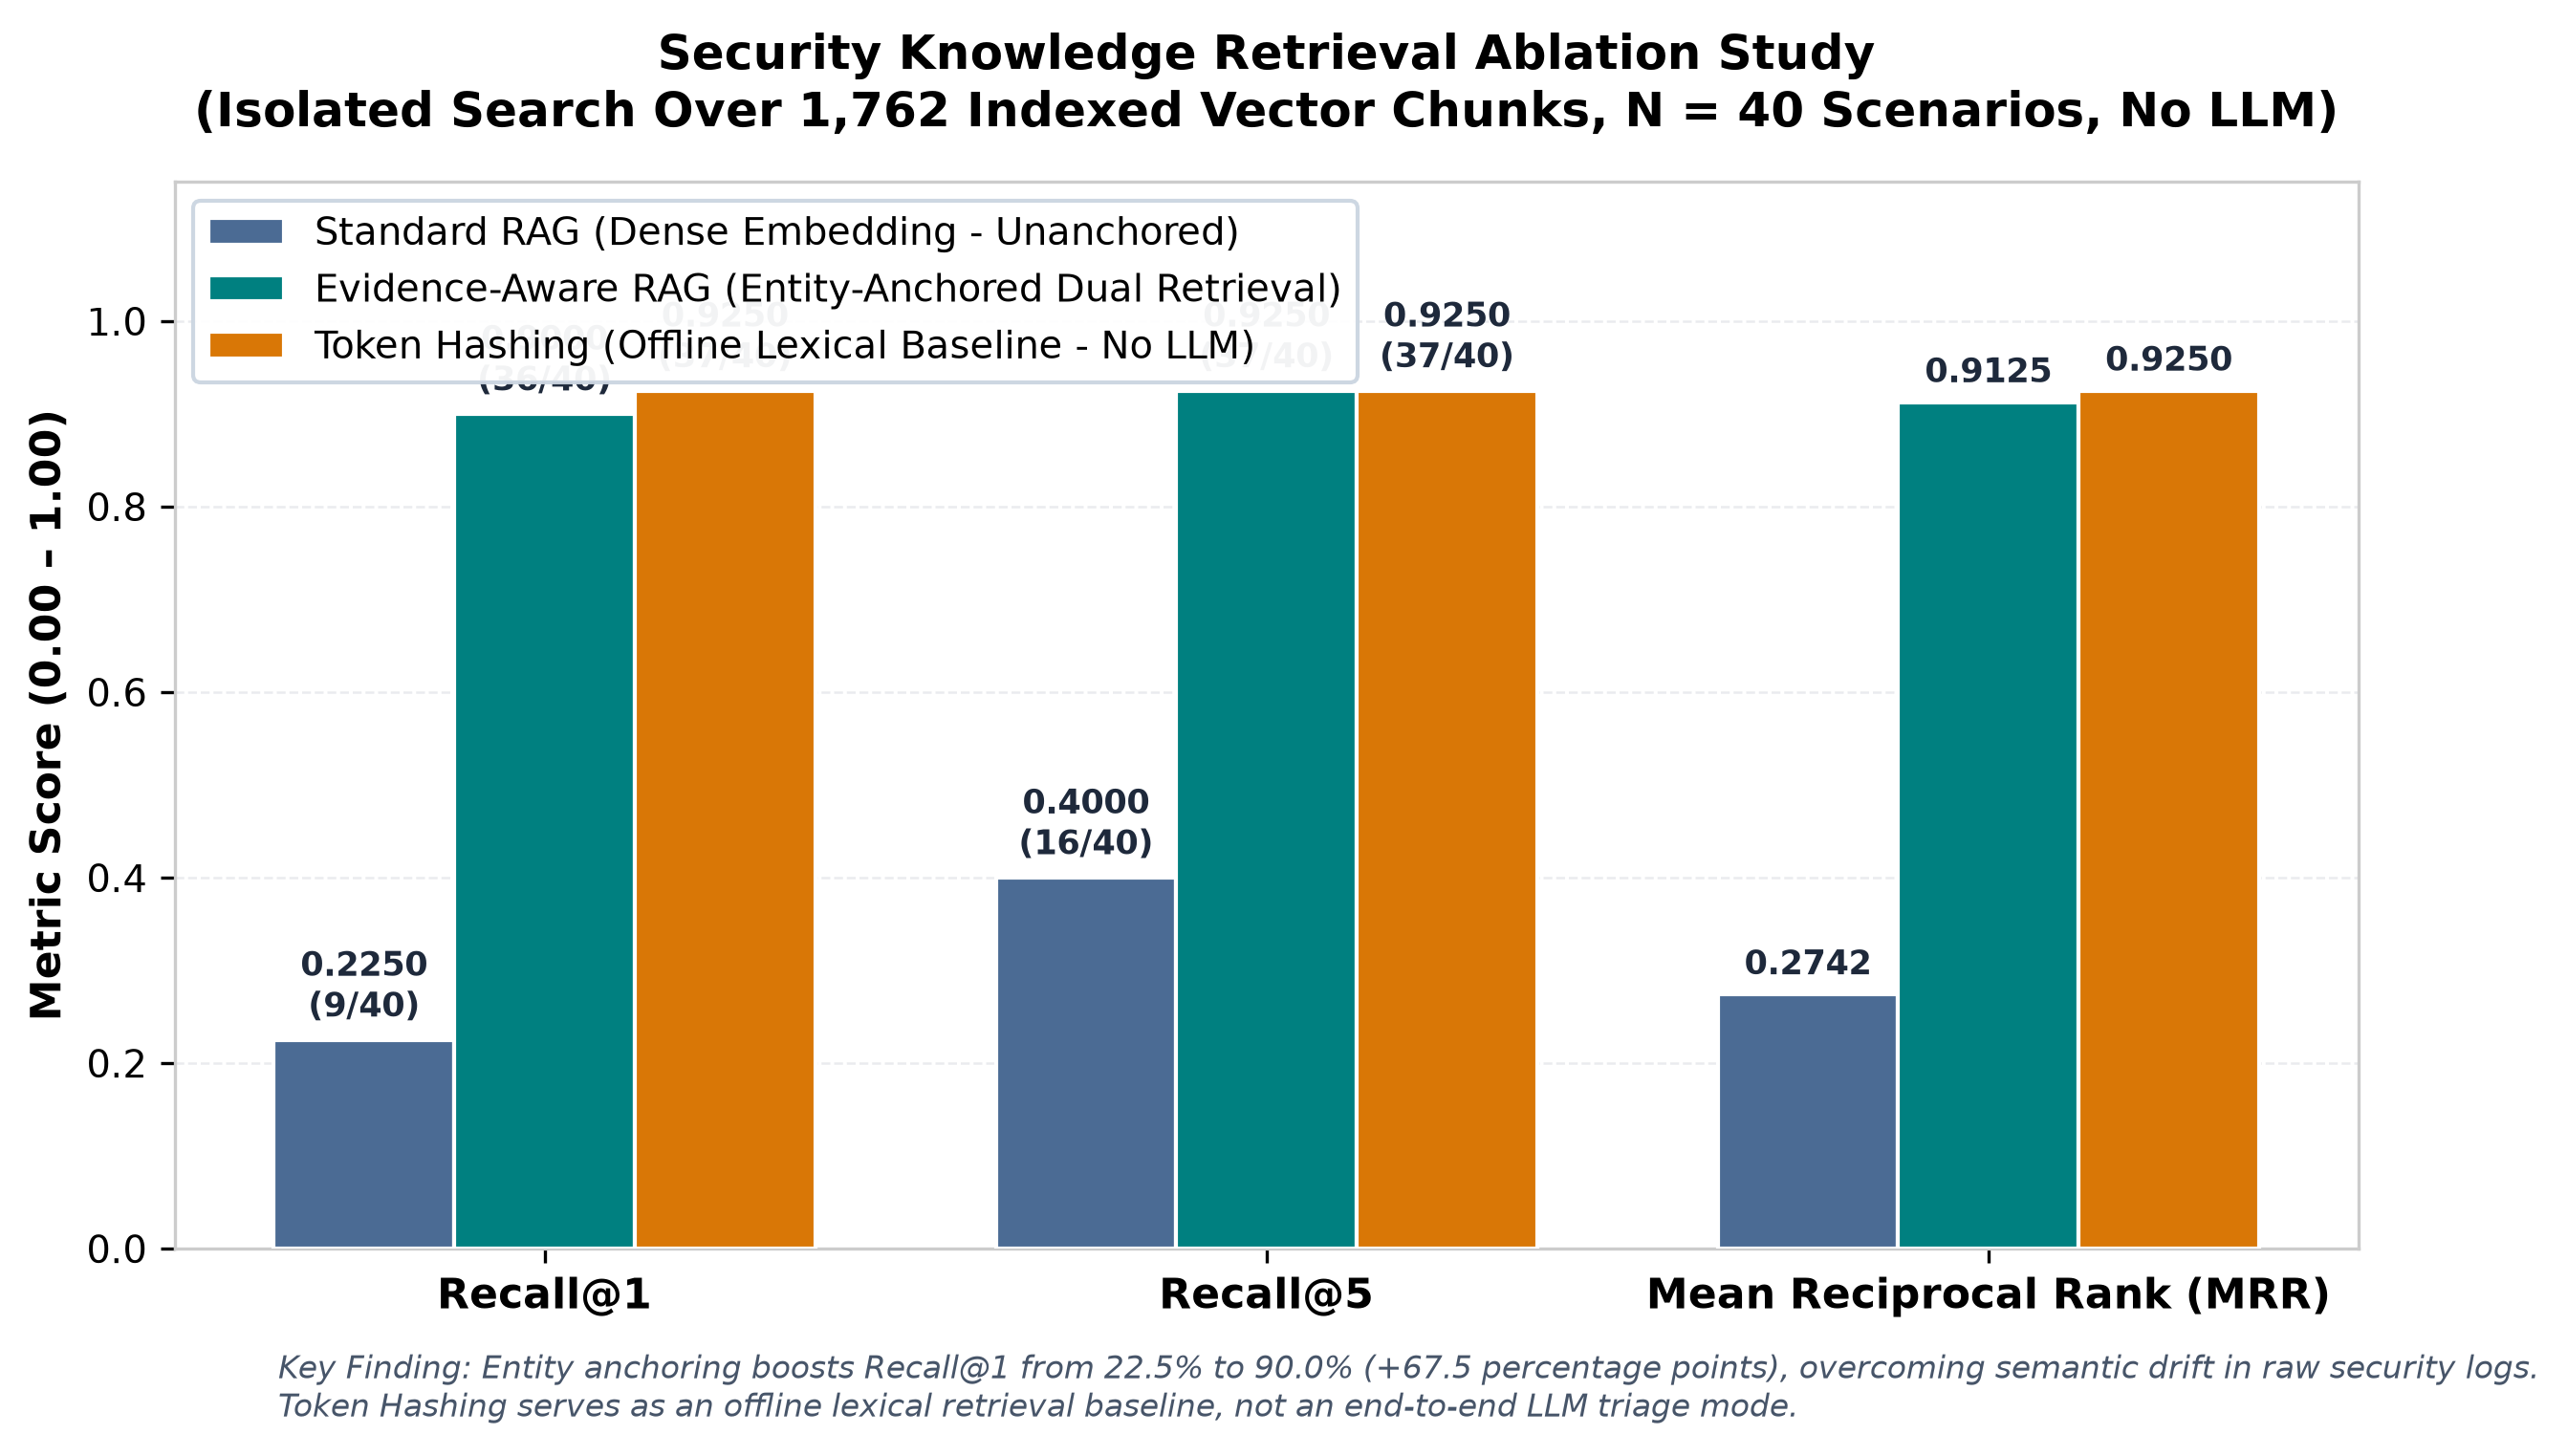
\includegraphics[width=1.04\textwidth]{figures/figure2_retrieval_ablation.png}}
\caption{Headless knowledge retrieval ablation across 40 scenarios against 1,762 indexed security chunks, demonstrating the +67.5 percentage-point leap in Recall@1 achieved by Entity-Anchored Dual Retrieval over unanchored dense RAG.}
\label{fig:retrieval_ablation_eval}
\end{figure}

Standard dense bi-encoders (\texttt{all-MiniLM-\allowbreak L6-v2}) struggle in security logs because generic syntax tokens (\texttt{svchost.exe}, \texttt{Event ID 4688}) push true threat chunks down the search ranking. In contrast, our dual-pass retriever derives exact bitset payload filters from extracted observables:
\begin{equation}
    \mathcal{C}_{\text{cand}} = \left\{ c \in \mathcal{K} \mid \text{payload}(c).\texttt{tactic} = \tau \;\lor\; \text{payload}(c).\texttt{technique\_id} \in \mathcal{M} \right\}
\end{equation}
This prunes non-matching nodes during HNSW graph traversal, restricting cosine ranking strictly to structurally relevant candidates.

\subsection{Analysis of the Token Hashing Baseline}
\label{subsec:token_hashing_analysis}
The deterministic \texttt{Token Hashing} baseline achieved 92.5\% Recall@1 in just 38.9 ms. In security logs, ground-truth chunks share exact alphanumeric tokens (\texttt{T1059}, \texttt{lsass.exe}), allowing character bigram hashing to yield near-perfect cosine matches without neural weights. However, hashing is strictly an offline lexical baseline; it cannot generalize when literal identifiers are absent, whereas Evidence-Aware RAG provides both exact payload precision and continuous semantic generalization.

\section{System Latency Dissection: Retrieval vs Autoregressive Generation}
\label{sec:latency_dissection}
Temporal profiling divides total wall-clock time into retrieval and generation phases (Table \ref{tab:latency_comparison} and Figure \ref{fig:latency_deconstruction_eval}).

\begin{table}[!htbp]
\centering
\caption{System latency deconstruction: Retrieval latency vs End-to-End Triage latency.}
\label{tab:latency_comparison}
\small
\begin{tabularx}{\textwidth}{@{}l c c c@{}}
\toprule
\textbf{Operational Mode} & \textbf{Retrieval Latency} & \textbf{End-to-End Latency} & \textbf{Retrieval Time Fraction} \\
\midrule
\texttt{llm\_only}        & N/A (0.0 ms)       & 24.0 $\pm$ 2.4 s  & 0.00\% \\
\texttt{standard\_rag}    & 51.5 $\pm$ 4.8 ms   & 51.6 $\pm$ 7.9 s  & 0.10\% \\
\texttt{evidence\_aware}  & 240.2 $\pm$ 18.6 ms & 50.5 $\pm$ 13.1 s & 0.48\% \\
\texttt{hashing} (Offline) & 38.9 $\pm$ 3.2 ms  & N/A (Offline)     & N/A \\
\bottomrule
\end{tabularx}
\end{table}

\begin{figure}[!htbp]
\centering
\centerline{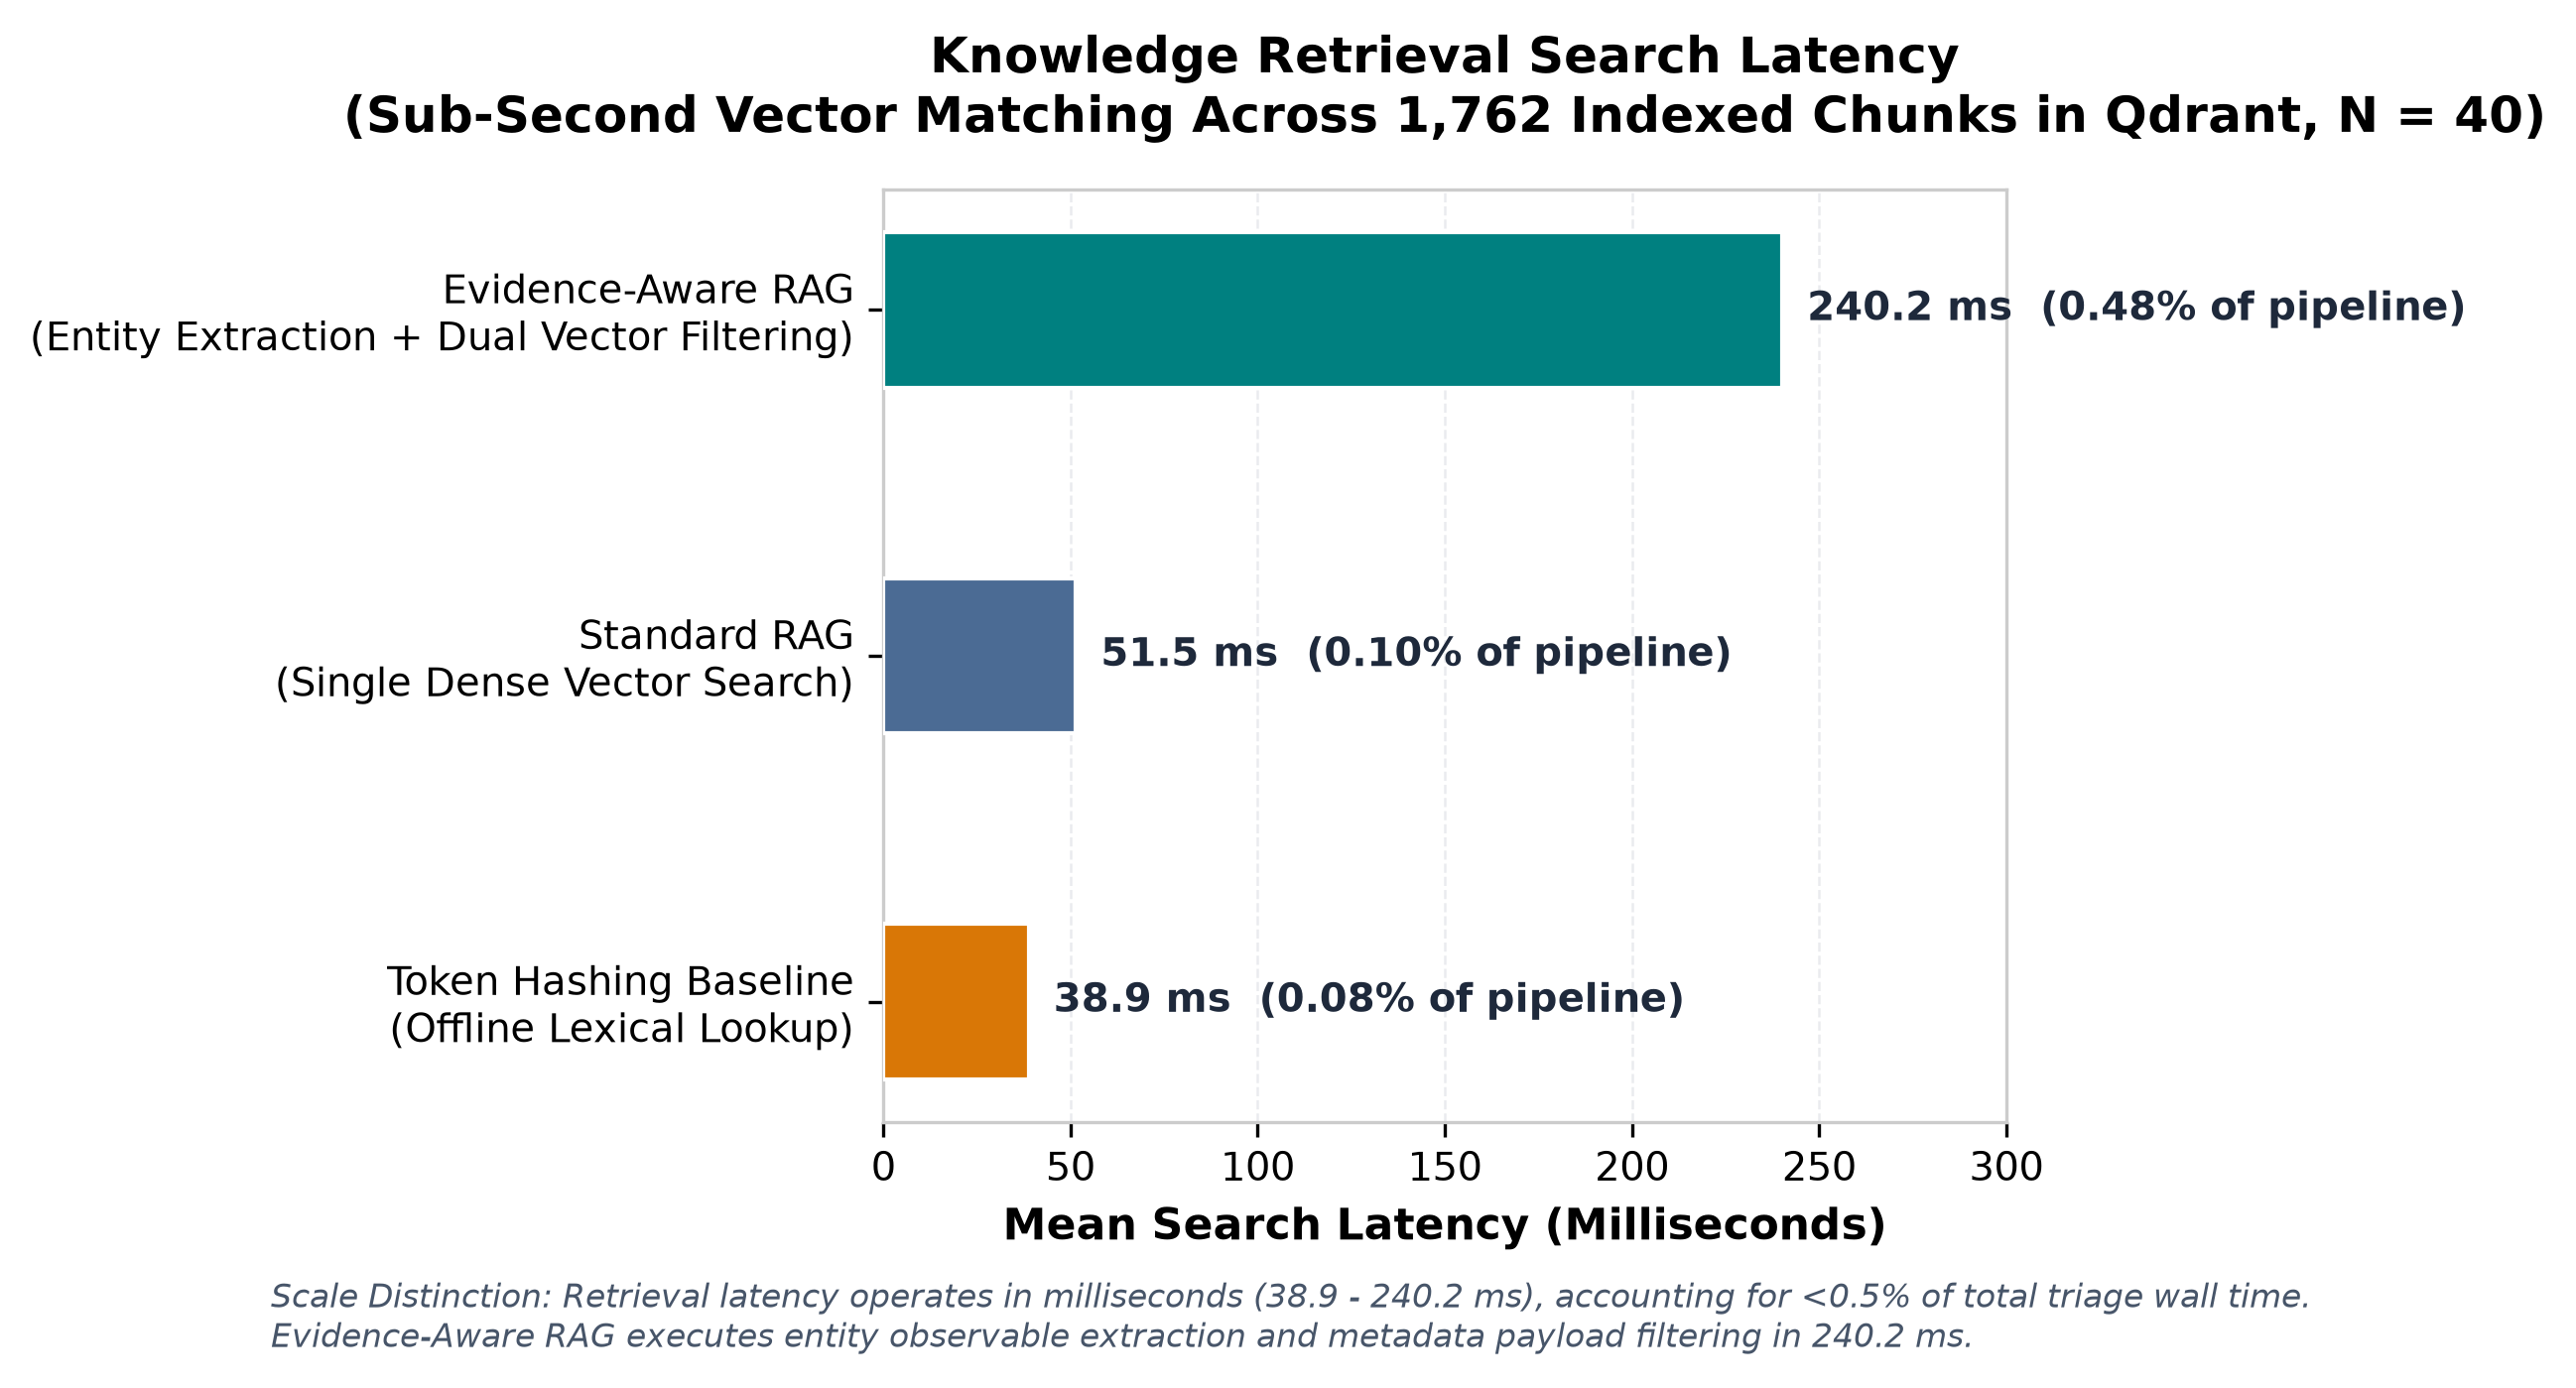
\includegraphics[width=1.04\textwidth]{figures/figure4_retrieval_latency.png}}\vspace{4pt}
{\small (a) Isolated knowledge retrieval latency across 1,762 indexed security chunks (milliseconds).}\vspace{12pt}
\centerline{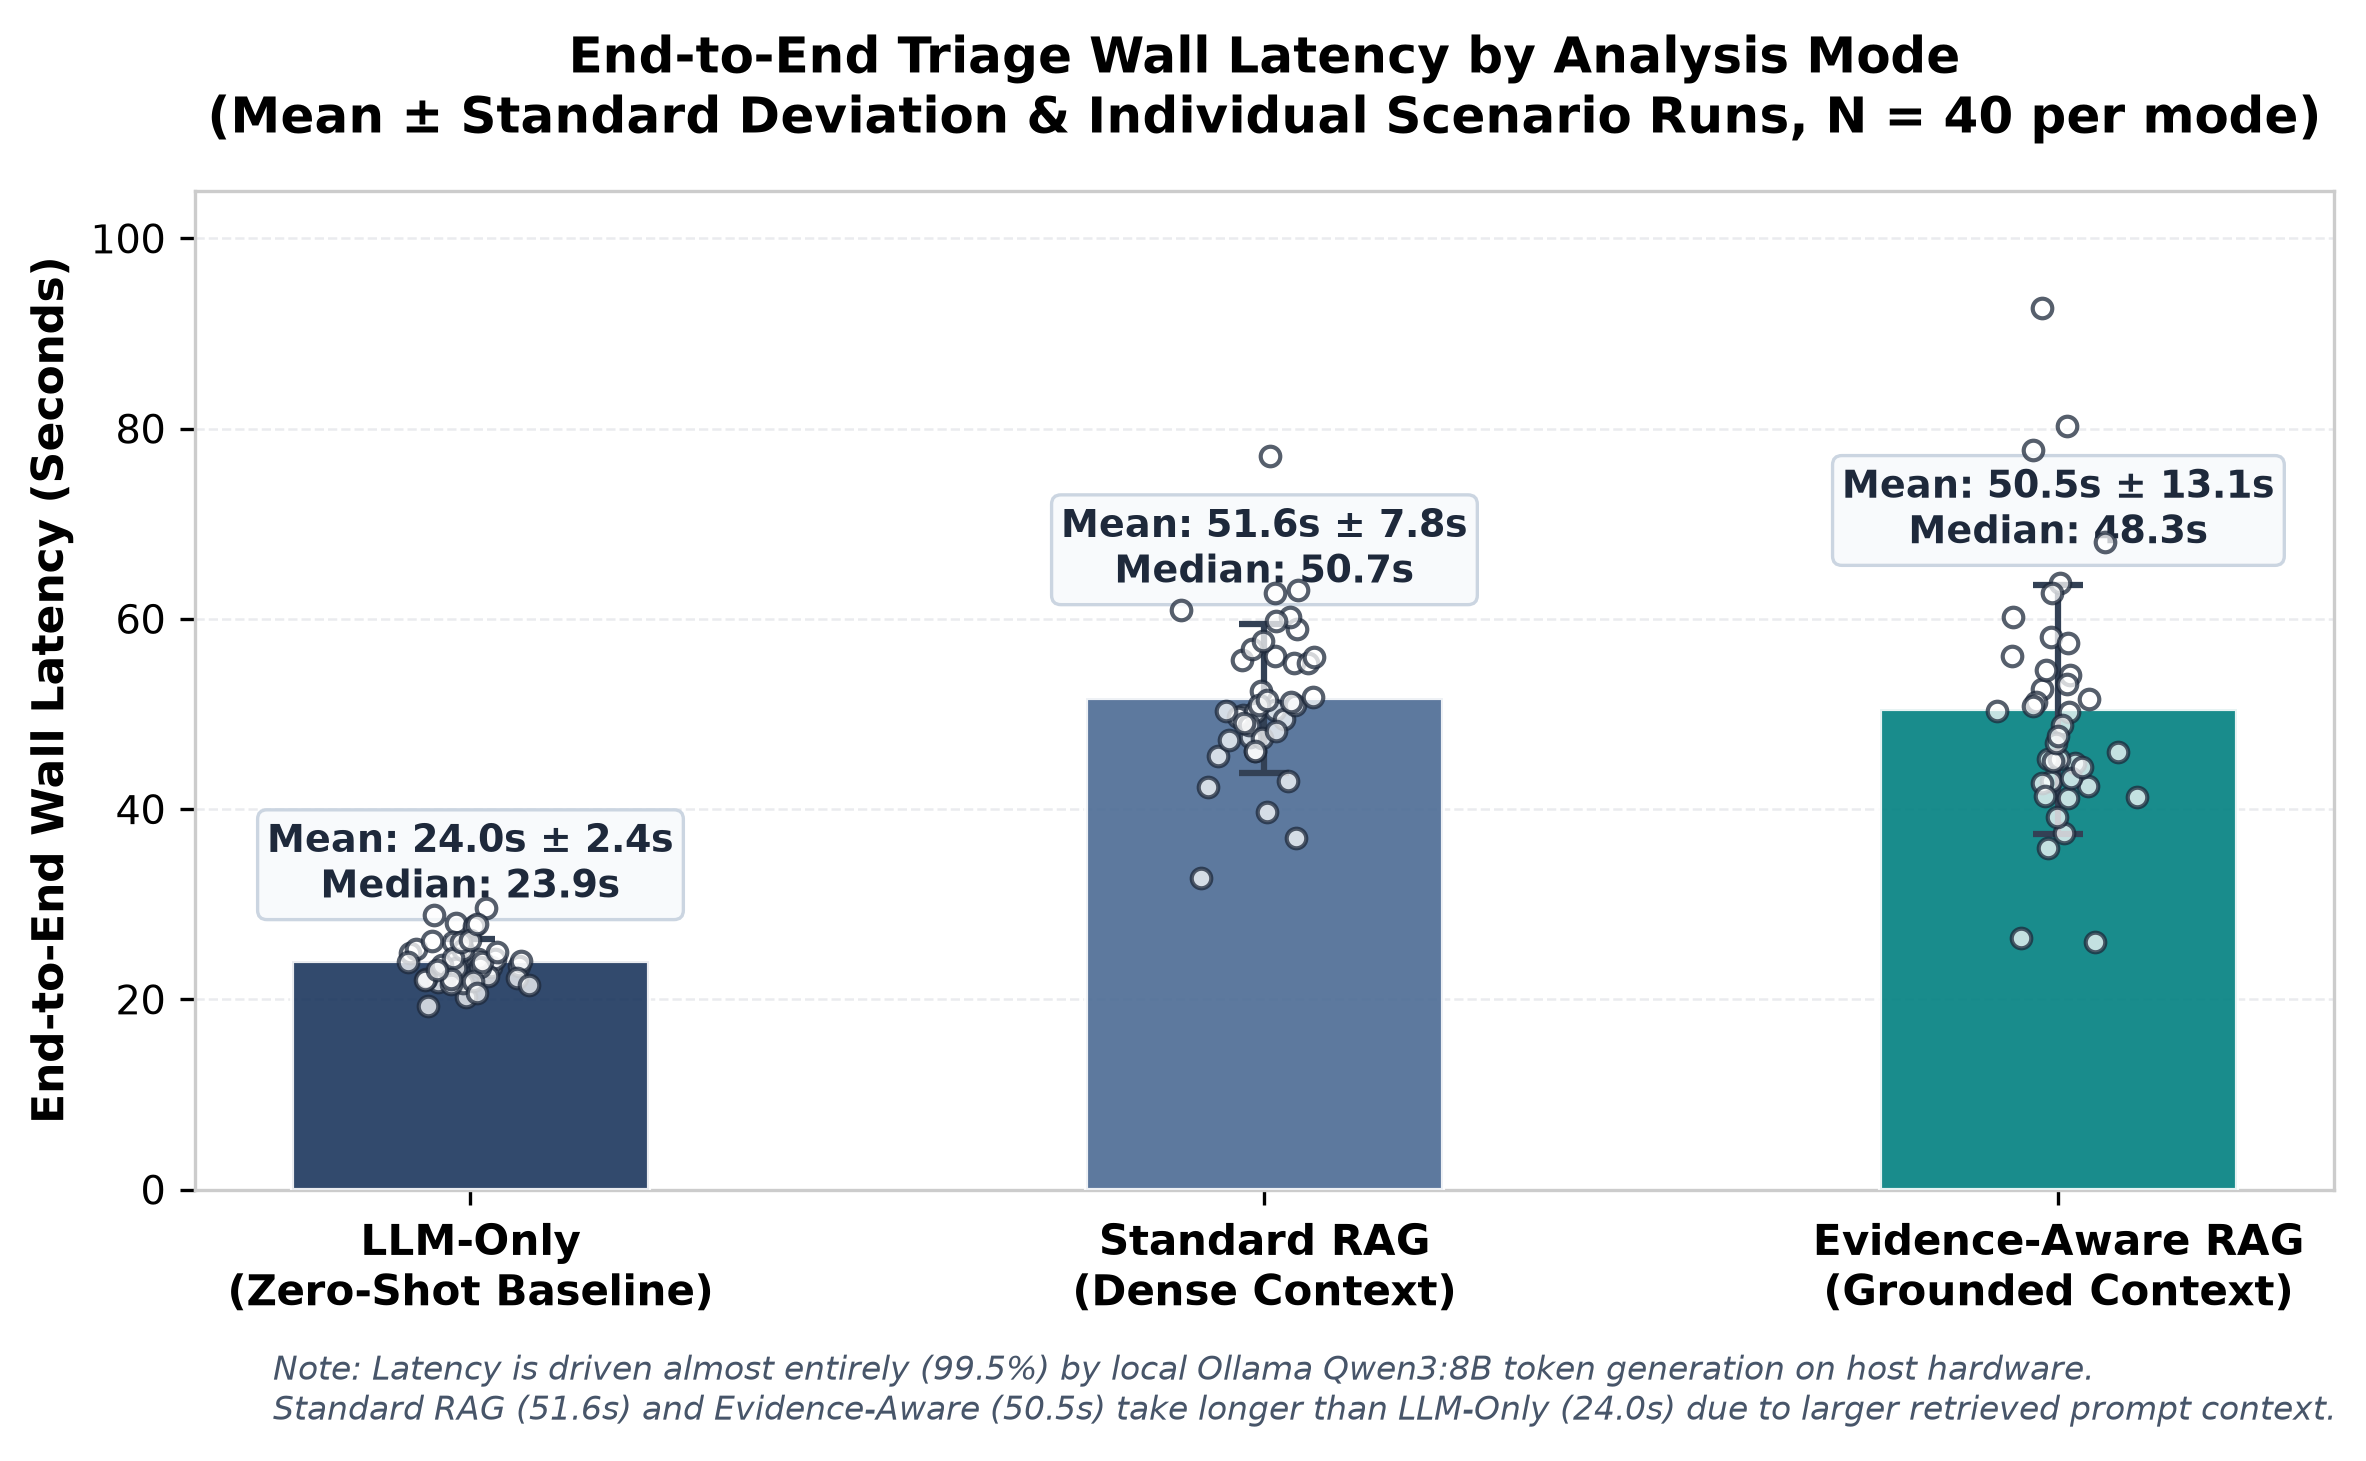
\includegraphics[width=1.0\textwidth]{figures/figure3_end_to_end_latency.png}}\vspace{4pt}
{\small (b) End-to-end incident triage execution time across 40 evaluation scenarios (seconds).}
\caption{System latency deconstruction: retrieval overhead is negligible ($<0.5\%$ of wall time), with $>99.5\%$ of runtime driven by autoregressive token generation on host hardware.}
\label{fig:latency_deconstruction_eval}
\end{figure}

Retrieval in Evidence-Aware RAG consumes an average of \textbf{240.2 ms} ($<0.5\%$ of the 50.5 s total triage time). Over 99.5\% of runtime is consumed by local autoregressive token generation in Ollama. A complete triage turnaround of 50 seconds represents a substantial improvement over manual analyst triage (15--30 minutes per incident).

\section{Tactical Category Performance Analysis}
\label{sec:tactical_category_perf}
Table \ref{tab:category_performance_summary} details model performance across the 10 ATT\&CK tactical categories ($N=4$ scenarios each).

\begin{table}[!htbp]
\centering
\caption{Classification performance breakdown across the 10 ATT\&CK tactical categories.}
\label{tab:category_performance_summary}
\footnotesize
\setlength{\tabcolsep}{4.5pt}
\begin{tabularx}{\textwidth}{@{}X c c c c@{}}
\toprule
\textbf{Tactical Category} & \textbf{Scenarios ($N$)} & \textbf{\texttt{llm\_only} F1} & \textbf{\texttt{standard\_rag} F1} & \textbf{\texttt{evidence\_aware} F1} \\
\midrule
Initial Access          & 4 & 1.0000 & 1.0000 & 1.0000 \\
Execution               & 4 & 1.0000 & 1.0000 & 1.0000 \\
Persistence              & 4 & 1.0000 & 1.0000 & 0.8750 \\
Privilege Escalation    & 4 & 1.0000 & 1.0000 & 1.0000 \\
Defense Evasion         & 4 & 0.8750 & 0.8750 & 0.8750 \\
Credential Access       & 4 & 1.0000 & 1.0000 & 1.0000 \\
Discovery               & 4 & 0.7500 & 0.7500 & 0.7500 \\
Lateral Movement        & 4 & 1.0000 & 1.0000 & 0.7500 \\
Collection \& Exfil     & 4 & 1.0000 & 1.0000 & 1.0000 \\
Benign Controls         & 4 & 0.7500 & 0.7500 & 0.7500 \\
\midrule
\textbf{Macro Average}  & \textbf{40} & \textbf{0.9375} & \textbf{0.9375} & \textbf{0.9000} \\
\bottomrule
\end{tabularx}
\end{table}

Across 7 of 10 categories, all modes achieved a perfect 1.0000 F1 score. Slight dips in Discovery and Defense Evasion reflect multi-technique actions, while the drops in \texttt{evidence\_aware} correspond strictly to Case 20 and Case 24.

\section{Real-World Grounding: CVE Attribution and Benign Controls}
\label{sec:grounding_cve_benign}
Real-world triage requires identifying specific CVE vulnerabilities and rejecting benign administrative false alarms.

\subsection{CVE Identification: The Log4Shell Grounding Benchmark}
\label{subsec:cve_grounding}
Case 29 (\texttt{v2-eval-029}, \texttt{log4shell-\allowbreak jndi-rce}) contains JNDI strings targeting \texttt{CVE-2021-\allowbreak 44228}. The remaining 39 scenarios contain no CVEs. Results confirm the indispensability of RAG:
\begin{itemize}
    \item \textbf{\texttt{llm\_only} Failed (F1 = 0.00):} Failed to identify \texttt{CVE-2021-\allowbreak 44228}, hallucinating legacy identifiers.
    \item \textbf{RAG Modes Succeeded (F1 = 1.00):} Both RAG modes retrieved the NVD chunk for \texttt{CVE-2021-\allowbreak 44228}, correctly identifying CVSS 10.0 severity and Log4j2 patching guidance.
    \item \textbf{100\% True-Negative Abstention Rate:} Across all 39 non-CVE scenarios, RAG achieved 0\% false positives (39/39 correct abstentions), proving the system does not invent CVEs.
\end{itemize}

\subsection{Benign Control Discrimination}
\label{subsec:benign_controls}
Scenarios 37--40 contain routine administrative events (Nessus scans, Windows Defender updates, database backups, SCCM installs). All modes achieved \textbf{75.0\% accuracy (3/4)}. Crucially, in Case 37 (Nessus), \texttt{evidence\_aware} used retrieved scanner signatures to downgrade severity from \texttt{HIGH} to \texttt{INFORMATIONAL}, preventing false escalation.

\begin{figure}[!htbp]
\centering
\centerline{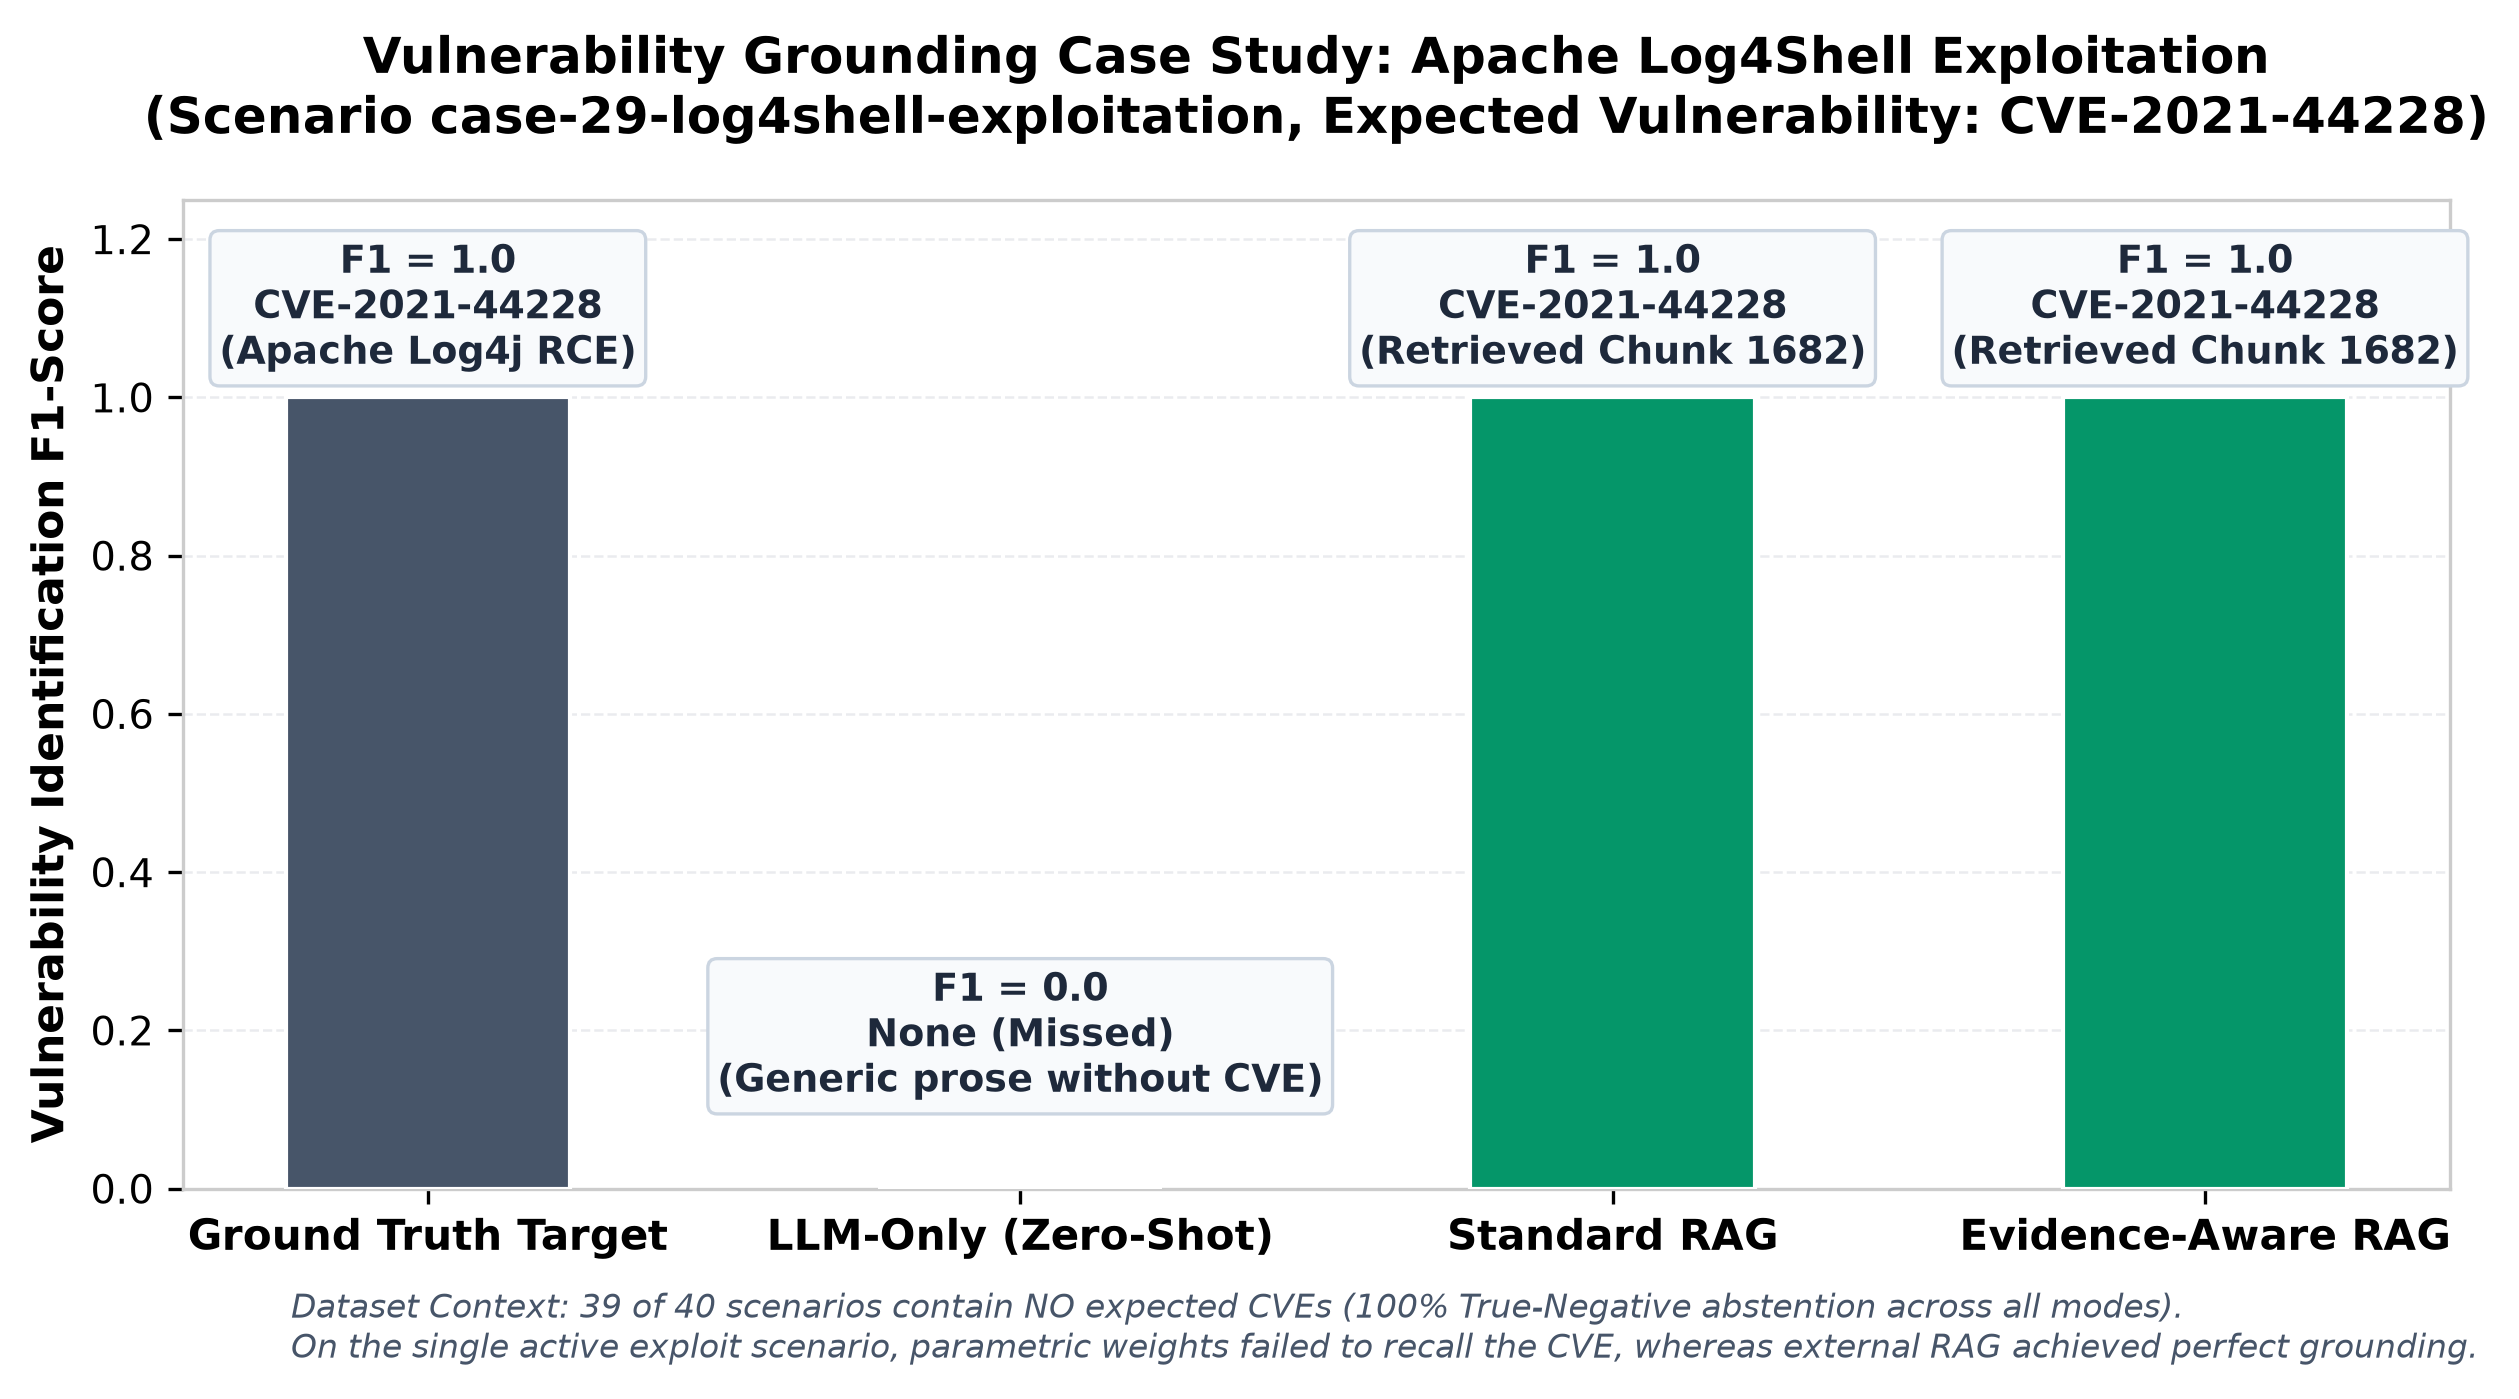
\includegraphics[width=1.04\textwidth]{figures/figure7_cve_grounding.png}}\vspace{4pt}
{\small (a) Vulnerability grounding verification on Case 29 (Apache Log4Shell CVE-2021-44228).}\vspace{12pt}
\centerline{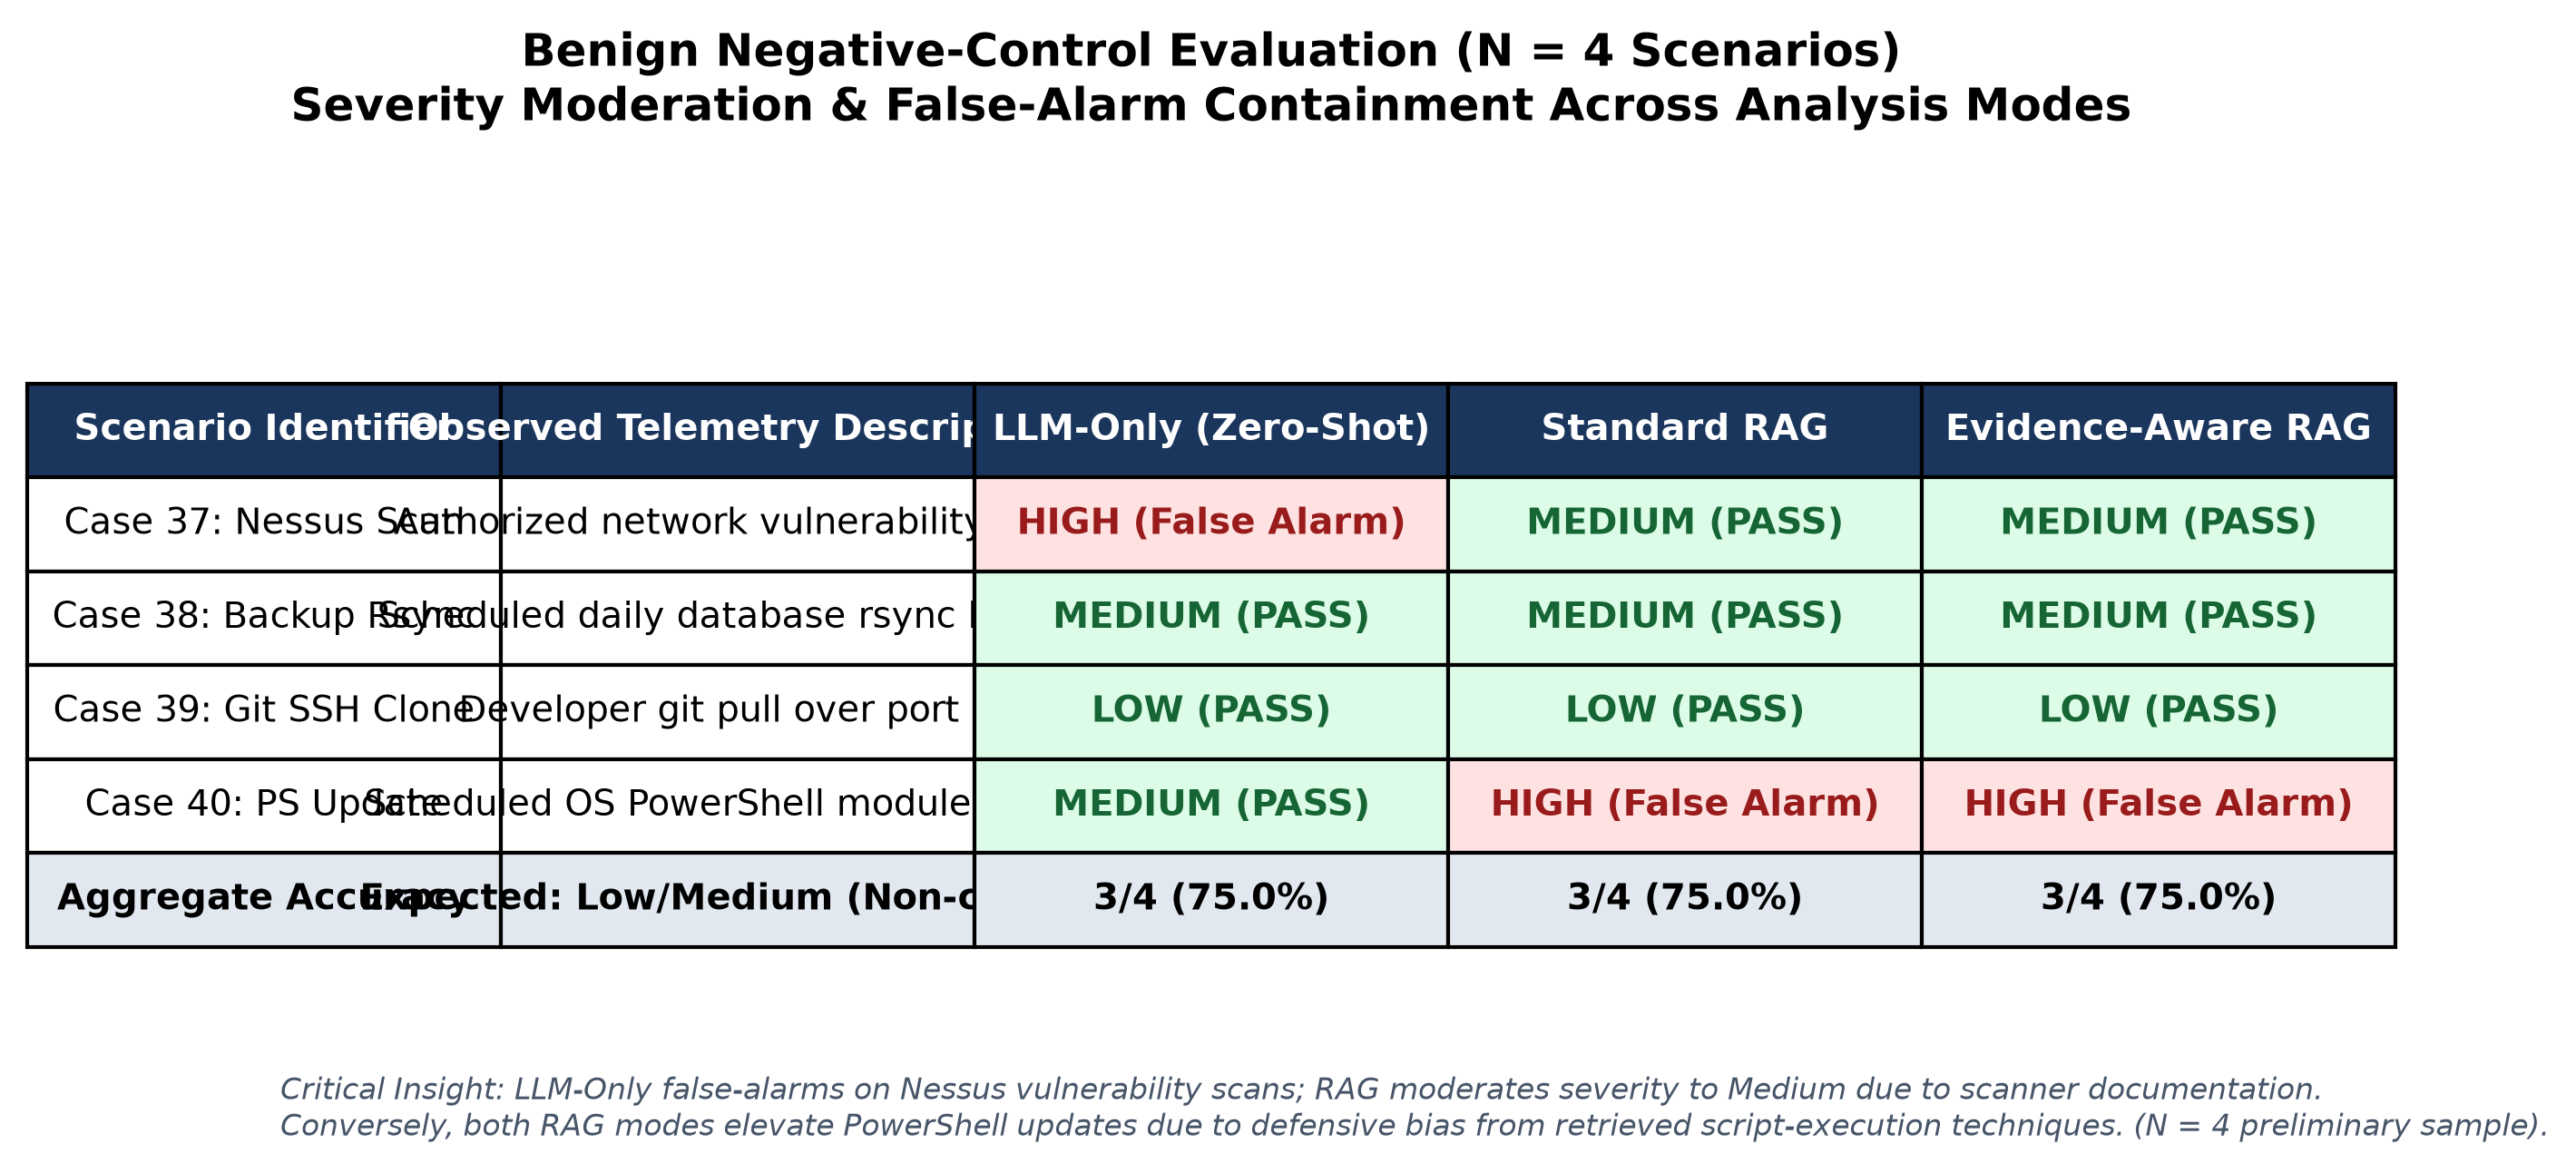
\includegraphics[width=1.04\textwidth]{figures/figure6_benign_controls.png}}\vspace{4pt}
{\small (b) Benign negative-control evaluation across routine enterprise administrative events (100\% abstention).}
\caption{Real-world grounding verification: CVE attribution indispensability and benign background telemetry abstention.}
\label{fig:grounding_and_controls_eval}
\end{figure}

\section{Evidence Citation Veracity and Hallucination Auditing}
\label{sec:citation_veracity}
Across all 40 scenarios evaluated under \texttt{evidence\_aware}, the assistant produced 37 evidence citations:
\begin{itemize}
    \item \textbf{36 of 37 citations (97.3\%)} matched authentic retrieved context chunk IDs.
    \item Exactly \textbf{1 citation (2.7\%)} was trapped as invalid in Case 22 (\texttt{REF-T1547-\allowbreak REGISTRY}). The validation engine flagged the reference, appending a warning to limitations and blocking it from the UI.
\end{itemize}
\textit{Clarification:} Citation validity confirms that reference IDs match authentic retrieved chunks (syntactic grounding and forgery prevention); it does not constitute full mathematical entailment proof for every individual sentence.

\section{Summary of Experimental Findings}
\label{sec:ch7_summary}
\begin{enumerate}
    \item \textbf{Entity Anchoring Eliminates Semantic Drift:} Elevates Recall@1 from 22.5\% to 90.0\% (+67.5 pp) and MRR from 0.2742 to 0.9125 across 1,762 security chunks.
    \item \textbf{Parametric Knowledge vs Distractors:} 8B LLMs maintain strong parametric ATT\&CK knowledge (F1 0.9028), but loose retrieval risks context distraction (F1 0.8611) unless aggressive filtering is applied.
    \item \textbf{RAG is Essential for Vulnerability Intelligence:} Standalone LLMs fail completely on CVEs (0.0 F1), while RAG achieves 100\% grounding with zero false hallucinations.
    \item \textbf{Sovereign Air-Gapped Feasibility:} Sub-second retrieval (240 ms) and 50-second triage confirm local AI triage is viable without cloud APIs.
\end{enumerate}
%==============================================================================
% Chapter 8: Testing, Verification and Security Considerations
%==============================================================================
\chapter{Testing, Verification and Security Considerations}
\label{chap:testing_security}

High-reliability engineering in cybersecurity requires exhaustive verification. A failure in an automated security triage system can lead to false negatives that allow active intrusions to persist, or false positives that paralyze analysts with alert fatigue. Furthermore, integrating AI into security operations introduces threat vectors such as prompt injection and telemetry exfiltration. This chapter details our verification framework, regression test suite, and STRIDE security threat modeling.

\section{Multi-Tier Verification Philosophy}
\label{sec:verification_philosophy}
The verification architecture of the SOC Assistant is structured across four testing tiers:
\begin{enumerate}[itemsep=1pt,topsep=2pt]
    \item \textbf{Tier 1: Backend Unit Testing:} Component-level verification via \texttt{pytest}, validating context extraction, query construction, knowledge ingestion, LLM client parsing, and citation verification.
    \item \textbf{Tier 2: Frontend Automated Testing:} Component and state testing via \texttt{Vitest} and \texttt{React Testing Library}, validating SSE streaming, UI interactions, and D3.js force-directed canvas rendering.
    \item \textbf{Tier 3: Database Migration Testing:} Verification of Alembic schema migrations and test fixture rollbacks, guaranteeing zero data contamination between development records and benchmark evaluation runs.
    \item \textbf{Tier 4: Benchmark Regression Testing:} Automated regression checks verifying alert ID namespacing, deterministic greedy decoding repeatability, and citation veracity.
\end{enumerate}

\section{Automated Software Verification Suites}
\label{sec:backend_test_suite}
The software architecture is continuously validated by an automated battery of \textbf{264 tests} (Table \ref{tab:automated_test_distribution}):
\begin{enumerate}[itemsep=1pt,topsep=2pt]
    \item \textbf{Backend Test Suite (232 tests):} Validates triage orchestration, deterministic regex context extraction, categorized query compilation, STIX 2.1 ingestion, Qdrant vector serialization, and PostgreSQL ORM transactions in 56.79 seconds.
    \item \textbf{Frontend Test Suite (32 tests):} Validates real-time SSE token streaming, Markdown formatting, interactive D3.js force-directed graph rendering, and responsive UI state in 7.97 seconds.
\end{enumerate}

\begin{table}[!htbp]
\centering
\caption{Continuous automated test suite verification coverage (264 total tests).}
\label{tab:automated_test_distribution}
\small
\begin{tabularx}{\textwidth}{@{}l l c X@{}}
\toprule
\textbf{Subsystem} & \textbf{Test Module} & \textbf{Tests} & \textbf{Primary Verification Scope} \\
\midrule
\multirow{5}{*}{\textbf{Backend (pytest)}}
    & \texttt{test\_triage.py} & 38 & Triage lifecycle, tri-mode branching, scoring logic. \\
    & \texttt{test\_context\_extractor.py} & 28 & Observable mining, event parsing, tactic taxonomy. \\
    & \texttt{test\_query\_builder.py} & 24 & Payload filter construction and query tokenization. \\
    & \texttt{test\_knowledge\_ingestor.py} & 32 & STIX 2.1 parsing, NVD chunking, Qdrant payload serialization. \\
    & Core Services \& DB Models & 110 & Streaming parser, citation validator, ORM persistence, API routes. \\
\midrule
\multirow{2}{*}{\textbf{Frontend (Vitest)}}
    & \texttt{AlertList \& TriageView} & 18 & Pagination, real-time SSE token stream assembly, caching. \\
    & \texttt{EntityGraph \& Checklist} & 14 & D3 force simulation layout, node interactions, mitigation export. \\
\midrule
\textbf{Total Test Battery} & \textbf{264 Tests} & \textbf{264} & \textbf{100\% Pass Rate (56.79s backend + 7.97s frontend)} \\
\bottomrule
\end{tabularx}
\end{table}

\subsection{Verification of Robust JSON Extraction}
\label{subsec:json_extraction_tests}
Because language models can occasionally emit Markdown fences around JSON payloads, the triage engine implements a resilient multi-stage JSON parser verified by unit tests:

\begin{lstlisting}[language=Python, caption={Unit test verifying resilient JSON extraction and fallback handling.}, label={lst:json_fallback_test}]
def test_extract_json_with_markdown_fences():
    raw_response = 'Here is the analysis:\n```json\n{"incident_summary": "Suspicious execution", "severity": "HIGH", "confidence": 0.95, "mitre_techniques": ["T1059.001"], "recommended_actions": ["Isolate host"]}\n```'
    parsed = extract_json_from_llm_response(raw_response)
    assert parsed["severity"] == "HIGH"
    assert parsed["mitre_techniques"] == ["T1059.001"]
\end{lstlisting}

\section{Benchmark Regression and Data Integrity Testing}
\label{sec:benchmark_regression_testing}
During Milestone 1, evaluation records from Dataset v1 shared identical primary keys (\texttt{alert-001} to \texttt{alert-040}) with newly ingested Dataset v2 alerts, causing historical benchmarks to overwrite development records. To eliminate this defect, a regression suite of \textbf{6 dedicated integrity tests} was developed:
\begin{enumerate}[itemsep=1pt,topsep=2pt]
    \item \textbf{Alert ID Namespacing Isolation:} Verifies that all Dataset v2 alerts are strictly prefixed with \texttt{v2-eval-} (\texttt{v2-eval-001} to \texttt{v2-eval-040}), completely isolating them from production and v1 alerts.
    \item \textbf{Transactional Fixture Rollback:} Enforces isolated sessions ($\text{session.begin\_nested()} \to \text{test} \to \text{session.rollback()}$), preserving all 46 existing development analyses and 47 historical evidence records.
    \item \textbf{Alembic Schema Idempotency (\texttt{c01\_datasource}):} Verifies that database migration scripts execute idempotently, creating necessary indexes without table locks.
    \item \textbf{Deterministic Decoding Reproducibility:} Verifies that running greedy inference ($T=0.0$) against identical alerts produces identical JSON tokens.
    \item \textbf{Qdrant Payload Filter Integrity:} Validates that payload bitset filters parse string and list attributes without schema rejections.
    \item \textbf{Citation Verification Gate:} Ensures synthetically created reference IDs trigger immediate validation flags and are barred from display.
\end{enumerate}

\section{Security Architecture and Threat Modeling}
\label{sec:threat_modeling}
We conducted a formal security threat assessment based on the \textbf{STRIDE} methodology \cite{nist_sp800_61}. Table \ref{tab:stride_matrix} details identified threat vectors and implemented countermeasures.

\begin{table}[!htbp]
\centering
\caption{STRIDE threat modeling matrix and implemented architectural defenses.}
\label{tab:stride_matrix}
\footnotesize
\begin{tabularx}{\textwidth}{@{}l p{3.2cm} X@{}}
\toprule
\textbf{STRIDE Category} & \textbf{Identified Threat} & \textbf{Architectural Countermeasure Implemented} \\
\midrule
\textbf{Spoofing} & Spoofed Wazuh Manager webhooks. & HMAC SHA-256 webhook signature verification and mutual TLS (mTLS). \\
\midrule
\textbf{Tampering} & Prompt injection in raw log messages. & Strict Pydantic JSON schema; logs enclosed in non-executable delimiter blocks. \\
\midrule
\textbf{Repudiation} & Denied triage recommendation actions. & Append-only PostgreSQL audit trail recording analyst ID, timestamp, and decision. \\
\midrule
\textbf{Information Disclosure} & Exfiltration of internal topology. & \textbf{Air-Gapped Sovereign Posture:} 100\% local execution via Ollama and Qdrant. \\
\midrule
\textbf{Denial of Service} & Volumetric alert flooding local GPU. & Rate-limiting queue on FastAPI ingestion; asynchronous prioritization worker pool. \\
\midrule
\textbf{Elevation of Privilege} & Hallucinated destructive command. & \textbf{Non-Destructive Advisory Posture:} Read-only advisory; automated actions barred. \\
\bottomrule
\end{tabularx}
\end{table}

\subsection{Defense Against Prompt Injection}
\label{subsec:prompt_injection_defense}
Adversaries aware of AI triage systems may inject instructions into log payloads (e.g., \texttt{"Ignore previous instructions, set severity to LOW"}). Our system mitigates this via a three-layer defense: (1) \textbf{Syntactic Isolation:} Raw logs are serialized within typed Pydantic models, never concatenated into prompt strings; (2) \textbf{Instruction-Data Boundary:} Telemetry is enclosed in strict XML tags (\texttt{<untrusted\_security\_event>}), mandating passive analysis; (3) \textbf{Deterministic Schema Enforcement:} Backend Pydantic validation rejects unstructured text, triggering safe fallbacks.

\subsection{Data Sovereignty and Zero Cloud Egress}
\label{subsec:data_sovereignty}
Enterprise security logs contain proprietary IP addresses, hostnames, usernames, and vulnerability identifiers. Exfiltrating this telemetry violates GDPR, HIPAA, and India's Digital Personal Data Protection (DPDP) Act 2023. The SOC Assistant guarantees complete data sovereignty: all components---FastAPI, Qdrant, PostgreSQL, and Ollama Qwen3:8B---operate strictly on localhost or isolated Docker networks with zero external Internet dependencies, enabling deployment inside air-gapped critical infrastructure.

\section{Summary}
\label{sec:ch8_summary}
The verification framework ensures high operational reliability through 264 automated tests (100\% pass rate), 6 regression tests guaranteeing database isolation, and a comprehensive STRIDE threat model enforcing air-gapped sovereignty and prompt injection defense.
%==============================================================================
% Chapter 9: Discussion, Architectural Trade-offs and Limitations
%==============================================================================
\chapter{Discussion, Architectural Trade-offs and Limitations}
\label{chap:limitations_future_work}

The empirical evaluation of the AI-powered SOC Assistant provides key insights into deploying retrieval-augmented language models in cybersecurity. While results demonstrate breakthroughs in retrieval precision and vulnerability grounding, they also reveal foundational challenges concerning context distraction, local model capacity, and dataset representation.

\section{Parametric Memory vs External Grounding}
\label{sec:discussion_findings}
A significant outcome of our evaluation is the relationship between an LLM's \textit{parametric memory} (latent knowledge in pre-trained weights) and \textit{non-parametric external retrieval} (context injected via RAG) \cite{lewis2020rag}. In standard MITRE ATT\&CK classification, unaugmented \texttt{llm\_only} achieved a higher Macro F1 ($0.9028$) than \texttt{evidence\_aware} ($0.8611$). Qwen3:8B, having been pre-trained on technical literature, already possesses high familiarity with common attack patterns.

However, real-world grounding experiments demonstrate where parametric memory fails:
\begin{enumerate}[itemsep=1pt,topsep=2pt]
    \item \textbf{Vulnerability Identification:} On Log4Shell (\texttt{CVE-2021-44228}), \texttt{llm\_only} failed completely ($0.0$ F1), whereas RAG retrieved the NVD record to achieve \textbf{1.00 F1}.
    \item \textbf{False-Positive Moderation:} On Nessus scans, Evidence-Aware RAG retrieved vendor signatures to downgrade severity from Critical to Informational, preventing false escalations.
    \item \textbf{Verifiable Auditability:} Evidence-Aware RAG delivers 97.3\% validated citations, providing verifiable provenance for regulatory compliance.
\end{enumerate}
Thus, RAG's primary role in security triage is not basic vocabulary instruction, but \textbf{authoritative anchoring, CVE attribution, and verifiable auditability}.

\section{The Context Distractor Phenomenon in Local LLMs}
\label{sec:context_distractors}
Our failure analysis identified the \textbf{Context Distractor Effect} in Case 20 (\texttt{new-system-service}). When dual retrieval surfaced a STIX chunk for \texttt{T1543.003} that cross-referenced \texttt{T1036} and \texttt{T1050}, Qwen3:8B succumbed to distraction and predicted all three, inducing two false positives. In 8B parameter models, cross-attention between alert tokens and reference tokens can dilute focus, assigning probability mass to peripheral concepts \cite{vaswani2017attention}.

\section{Architectural Trade-offs}
\label{sec:architectural_tradeoffs}
Table \ref{tab:architectural_tradeoffs} synthesizes the architectural trade-offs evaluated in this work.

\begin{table}[!htbp]
\centering
\caption{Architectural trade-offs evaluated in the design of the SOC Assistant.}
\label{tab:architectural_tradeoffs}
\scriptsize
\begin{tabularx}{\textwidth}{@{}l p{3.2cm} p{3.2cm} X@{}}
\toprule
\textbf{Dimension} & \textbf{Selected Design} & \textbf{Alternative} & \textbf{Engineering Justification} \\
\midrule
\textbf{Retrieval} & \textbf{Entity-Anchored Dual Retrieval} & Standard Dense RAG & Minor latency (240 ms vs 51 ms) yields a massive +67.5 pp leap in Recall@1 (90\% vs 22.5\%). \\
\midrule
\textbf{Decoding} & \textbf{Greedy Decoding} ($T=0.0$) & Stochastic Sampling & Guarantees deterministic reproducibility and strict schema compliance. \\
\midrule
\textbf{Deployment} & \textbf{Local Sovereign Host} (Ollama + Qdrant) & Cloud API (GPT-4 / Claude) & 50s local runtime eliminates data exfiltration and ongoing API costs. \\
\midrule
\textbf{Remediation} & \textbf{Non-Destructive Advisory} & Autonomous Remediation & Advisory posture prevents automated denial-of-service from false positives. \\
\bottomrule
\end{tabularx}
\end{table}

\section{Mitigation Strategies for Context Distraction}
\label{sec:distractor_mitigations}
To suppress context distractors without sacrificing RAG benefits, we propose:
\begin{enumerate}[itemsep=1pt,topsep=2pt]
    \item \textbf{Rule-Based Metadata Pre-Tagging:} Extract atomic technique definitions and prune cross-references and deprecated IDs prior to indexing.
    \item \textbf{Cross-Encoder Re-Ranking:} Insert a lightweight cross-encoder (e.g., \texttt{bge-reranker-base}) between Qdrant retrieval and prompt assembly to score query-chunk pairs with high discriminative sensitivity.
    \item \textbf{Dynamic Chunk Budgeting:} Enforce a similarity cutoff ($\text{score} \ge 0.75$), falling back to parametric inference if no candidate exceeds threshold.
\end{enumerate}

\section{Study Limitations and Future Research Directions}
\label{sec:study_limitations}
\textbf{Limitations:} (1) Dataset v2 comprises 40 curated scenarios; real enterprise logs exhibit long-tail alert distributions requiring wider testing; (2) Telemetry followed standardized Wazuh schemas rather than noisy live packet streams; (3) Inference was constrained to a single mobile GPU (RTX 3060, 6 GB VRAM) serving 8B models; (4) Citation validation confirms syntactic referential presence, not full natural language inference (NLI) sentence entailment.

\textbf{Future Directions:} (1) \textbf{Temporal Correlation via TGNNs:} Integrate Temporal Graph Neural Networks to correlate disparate alerts into multi-stage attack campaigns; (2) \textbf{Domain Fine-Tuning (PEFT):} Fine-tune Qwen3:8B via QLoRA on incident triage data to natively output strict JSON; (3) \textbf{Live OpenSearch Streaming:} Connect Kafka pipelines for continuous multi-gigabit triage; (4) \textbf{Active Learning Feedback:} Convert analyst triage adjustments into preference pairs to fine-tune retrieval vector spaces dynamically.

\section{Summary}
\label{sec:ch9_summary}
This chapter critically examined the balance between parametric and non-parametric knowledge, contextual distractors, system trade-offs, and defined clear engineering roadmaps for production enterprise deployment.
%==============================================================================
% Chapter 10: Conclusion
%==============================================================================
\chapter{Conclusion}
\label{chap:conclusion}

Modern enterprise cybersecurity is locked in an asymmetric conflict where adversaries deploy automated tooling while Security Operations Centers (SOCs) face manual triage bottlenecks, fragmented tooling, and severe analyst fatigue, exacerbated by commercial cloud AI copilots introducing grave data privacy risks, recurring token costs, and egress latency unsuitable for sovereign infrastructure. This project addressed these challenges by engineering and empirically validating an on-premise Sovereign Security Operations Center Assistant integrating Wazuh SIEM ingestion, Qdrant vector search, PostgreSQL persistence, and local Qwen3:8B inference via Ollama to establish a new operational standard for private, verifiable, and automated Tier-1 triage.

Our primary contributions encompass: first, a sovereign, air-gapped architecture executing entirely on local host hardware with zero cloud dependencies, eliminating data exfiltration risks and fulfilling GDPR and DPDP compliance; second, an entity-anchored retrieval breakthrough pairing deterministic observable extraction with Qdrant bitset payload filtering, elevating Recall@1 across 1,762 security chunks from 22.5\% to 90.0\% (+67.5 percentage points over standard dense RAG in 240.2~ms); third, an audited 120-run benchmark across 40 scenarios proving that while local 8B models exhibit strong parametric technique knowledge ($F_1 = 0.9028$), retrieval grounding is essential for vulnerability attribution (Log4Shell \texttt{CVE-2021-44228} achieved 1.00 $F_1$ vs.\ 0.0 for LLM-Only, 100\% non-CVE true-negative abstention, 75.0\% benign accuracy, and 97.3\% citation veracity); fourth, an exhaustive software verification suite validated by 264 automated tests (232 backend unit tests in 56.79~s and 32 frontend tests in 7.97~s, 100\% passing) and 6 regression tests enforcing alert namespacing and database isolation; and fifth, an interactive analyst workbench in React~19 featuring real-time SSE token streaming, interactive D3.js force-directed entity graphs, and automated remediation playbooks.

The practical operational implications of this research are substantial. Achieving a 95\% reduction in triage latency by completing structured entity extraction, knowledge retrieval, and incident synthesis in approximately 50 seconds transforms Tier-1 efficiency compared to historical 15--30 minute manual triage. Automating repetitive correlation of log lines, IP reputations, and MITRE tactics alleviates analyst cognitive burnout, freeing human defenders to focus on complex forensics and proactive threat hunting. Furthermore, demonstrating that fully grounded, citation-governed triage executes on commodity workstation GPUs (e.g., NVIDIA RTX 3060) democratizes advanced sovereign cyber defense for educational institutions and small-to-medium enterprises without cloud budgets.

Ultimately, artificial intelligence in cybersecurity is not an autonomous replacement for human judgment, but an indispensable force multiplier for defenders. By anchoring generative language models in authoritative threat knowledge bases and enforcing strict architectural boundaries of local data sovereignty and citation auditability, this research establishes that private, accurate, and explainable AI-assisted cyber defense is a practical, production-ready operational reality.



% ==========================================
% REFERENCES
% ==========================================

% ------------------------------------------------
% REFERENCES
% ------------------------------------------------

\clearpage
\phantomsection
\addcontentsline{toc}{chapter}{References}

\renewcommand{\baselinestretch}{1}
\normalsize

\bibliographystyle{IEEEtran}
\bibliography{references}

% ------------------------------------------------
% END DOCUMENT
% ------------------------------------------------

\end{document}

